\chapter{Experiments}

In this chapter we describe how the chosen song encoding methods were implemented. This includes describing the input, training (if there was any) and output (meaning the vector-encoded representations for each song in our 16594 songs dataset). We also acquaint the reader with our evaluation methods, the reason we decided to use them and the evaluation results for each method. The results are first presented separately for each method (or a group of closely related methods) and then summarized and most importantly interpreted in the \ref{sec:discussion} where various graphs and tables illustrating the prominent or interesting trends and tendencies can be found. Before all this however, we start with stating what the expected outcomes were before we even started.

\section{Expectations}

Even before reading any literature, we made two main predictions. 
\begin{itemize}
    \item \textbf{First:} Audio-based methods will perform better than text-based methods.
    \item \textbf{Second:} More advanced methods will outperform simpler machine learning methods.
\end{itemize}
These were based on our intuition and later also supported by reading into this topic, where most of the papers we studied were describing neural networks performing similar audio or text-based recommendation or classification and their results were compared to simpler algorithms. However, this has not proven to be accurate with our evaluation dataset. The reasons for why it might be the case are described at the end of this chapter in the \textbf{Discussion} section. \\
We were also hoping, that the text-based methods will not be complete irrelevant. In this case, we were right, but only to the extend that the text-based methods are not irrelevant in comparison to the audio-based methods. Overall, all the methods have shown that they seem to lack the properties to be useful as methods for recommendation.
\section{Evaluation}

\subsection{Wanted recommender-system features}
We already touched this in the introduction but it is useful to revise what we want from a good recommendation system and what its most important features are. Let's skip the software part for now (as it will be discussed further in the \textbf{Web application} chapter and focus purely on what it recommends. Probably the most crucial property a recommendation system should have is that it should include the items the user actually likes between the first 10 to maybe 50 recommendations. Because it does not really matter if an item the user would like ends up on the 500th or 5000th position. People rarely go that deep. \\
Another thing we would want is for the system to be able to improve its recommendations with a rising amount of data it acquires about a user. In our case this means, that we would expect the predictions to be better for users with longer playlists. \\
Even though the whole idea of this thesis is to approach recommendation more loosely, we still want our methods to posses these features to at least some reasonable extend. Also, as these are the properties other recommendation systems are being evaluated on, we can gain a better understanding of the features our methods share with other recommendation techniques as well as their where they differ. 
\subsection{Evaluation measures}
To test the wanted features described in the section above we performed evaluation as follows. \\
Our dataset contains 11123 playlists that were used to evaluate our algorithms. We chose to evaluate our algorithms only on playlists of length at least four. For each method, we did a 5-cross-validation where in a validation epoch, every playlists $p_i$ was divided into two parts a training part $p_{i_{train}}$ and a testing part $p_{i_{test}}$ with an approximately 80:20 ratio. A higher priority was set on the fact that the test part always had to contain at least one entry (meaning that for playlists of length 2, the ratio would be 50:50). \\
Afterwards for each song $ s_k $ from our song dataset $S$, the similarity of the whole $p_{i_{train}}$ to $s_k$ which we denote as $ sim(p_i, s_k) $ was calculated as $sim(p_i, s_k) =$ $\sum_{s_j\in{p_i{_{train}}}} cos_sim(s_i, s_j) $ where $ i \neq j$ and $cos_sim$ is the cosine similarity as defined by Python scikit-learn package. These similarities were then sorted and it was determined at what position the songs from $p_{i_{test}} $ that actually belong to the playlist came. \\
These positions were then used to calculate multiple evaluation measures used to assess how well does each algorithm predict the missing part of a users playlist. For this we chose the following for methods:
\begin{itemize}
    \item Recall at 10 (= \textbf{R@10}) defined as the number of songs from $p_{i_{test}} $ that placed in the top ten most similar songs.
    \item Recall at 50 (= \textbf{R@50}) defined as the number of songs from $p_{i_{test}} $ that placed in the top fifty most similar songs.
    \item Recall at 100 ( = \textbf{R@100} ) defined as the number of songs from $p_{i_{test}} $ that placed in the top hundred most similar songs.
    \item Normalized cumulative discounted gain (= \textbf{nCDG}) defined as 
    $${nDCG_{r}} = \frac{DCG_{r}}{IDCG{r}} $$
    where 
    $${DCG_{r}} =\sum_{i=1}^{r}{\frac {rel_{i}}{\log _{2}(i+1)}} $$ 
    is the discounted cumulative gain at position r and 
    $$ {IDCG_{r}} =\sum _{i=1}^{|REL|}{\frac {2^{rel_{i}}-1}{\log _{2}(i+1)}} $$
    is the ideal discounted cumulative gain at r
    where $r$ is in our case the number of songs that had to be predicted, the $rel_i$, meaning relevance, is the same for all songs as all songs in one playlists have the same relevance and $|REL|$ is the list of relevant items (in our case the songs from $p_{test}$).
    \item Average rank of a song from the $p_{i_{test}}$ set $ \boldsymbol{ (= \overline{rank})} $ which we included after the first four mentioned did not really meet our expectations.
    \item A graph plotting the distribution of rankings of songs from the test part of each playlists which we called the \textit{RDG} (=\textit{rank distribution graph}). We summed the number of songs from $p_test$ to which each individual rank from 1 to 16594 and divided it by the number of all songs that were in a testing part of some playlist. So for example if we had two playlists both with two songs from $p_{test}$ and our method assigned ranks 30 and 2900 to the $p_{test}$ songs from the first playlist and 2900 and 4872 to those from the second playlists, our graph would plot the values 0.25 for rank 30, 0.5 for rank 2900 and 0.25 for rank 4872 and 0 for the rest of the ranks. We did this for all playlists together but we also plotted the distributions for chosen playlist lengths separately to see if our predictions improve for longer playlists as we were hoping for. The x-scale of the \textit{RDG} was scaled logarithmicaly as we are much more interested in what is going on on the first 100 positions than what is goint on in the middle or towards the end. 
    
\end{itemize}
We calculated each of the first four measures for each playlist and then averaged over the whole playlist dataset. Every method section contains a table with the four measure averages and a graph. Both are accompanied with a short summary of the most obvious observations

To make things more easy for the rest of the thesis we introduce a nomenclature for our experimental methods. There are 3 different parts each of our method has. The name of the main algorithm, the name of the input and the length of the output vector. Every method can be uniquely identified by a combination of these three parts. Where there is only one or two of these necessary, we omit those which are surplus.\\
So for example a PCA method with spectrogram input and the output vector length of 320 is denoted as PCA\_spec\_320. If we take a look at the notation of the Tf-idf method, it will be only Tf-idf as there are no variations to it. However the PCA with Tf-idf input will be PCA\_Tf-idf. We separate the name parts with '\_' 

Just before we dive into the description of each method and it's results, 
\section{Text method experiments}

\subsection{TF-idf experiments}\label{ssec:TF_idf}


\subsubsection{Input}
The lyrics for each song were stripped of all punctuation characters as well as apostrophes, converted into a single string. 
\subsubsection{Training}
Each lyric-string was appended to the whole training dataset which was then passed to an instance of \texttt{sklearn.feature\_extraction.text.TFidfVectorizer} where the method \texttt{fit\_transform} was called. The results were saved into a numpy file containing a sparse matrix. And the model was saved using pickle.\\

\subsubsection{Output}
The song representation were vectors of length 40165 which is the number of different words our dataset contained.

\subsubsection{Results}

The results of the TF-idf method were poor overall when it comes to satisfying the properties of recommender systems.In comparison to our other methods however, they placed well above average. \\

\begin{table}[h!]
\centering
\renewcommand{\arraystretch}{1.5}
\begin{tabu} to 1\textwidth {| c || X[c] | X[c] | X[c] | X[c] | X[c] | }
 \hline
 \textbf{method} & \textbf{R@10} & \textbf{R@50} & \textbf{R@100} & \textbf{nGDC} & $ \boldsymbol{\overline{rank}} $ \\
 \hline
 \hline
 Tf-idf & 0.04293 & 0.05051 & 0.05619 & 0.03594 & 7553 \\
 \hline
 PCA on Tf-idf & 0.05091 & 0.05909 & 0.06393 & 0.04107 & 7345 \\
 \hline
\end{tabu} \\
\caption{Table summarizing average TF-idf and Tf-idf with PCA values averaged over the 5 cross validation that were performed}
\label{table:1}
\end{table}

When looking at the number in \ref{table:1} we can see that only 4.3\% of songs that were in our $p_{test}$ sets ranked in the first ten, 5\% in the first fifty and 5.6\% in the first hundred. The average rank of a song from our $p_{test}$ was 7553 which is quite close to the middle. This does not really satisfy our goals that we set to achieve in recommender systems. We also crated a \textit{RDG} as one can see in Figure \ref{fig:tf_idf_distribution}. It appears that according to the distribution, a song is more likely to end up in the first 10-100 songs than it is at the end. One could claim that this distribution is not random and favors ranks at the beginning, however not as strongly as we would want.\\
Another thing to notice in \ref{fig:tf_idf_distribution} is that there is a general trend for the Tf-idf method to perform worse on playlists with a greater length. This is the complete opposite of what we desire. One can see, that for playlists with length from 4 to 6, the ranks predicted for the missing songs were more likely to be higher than for playlists of length 21 and longer. The pink bar shows the overall distribution over 5000 bins over the dataset. 

\begin{figure}[h]
\centering
\begin{minipage}{.5\textwidth}
  \centering
  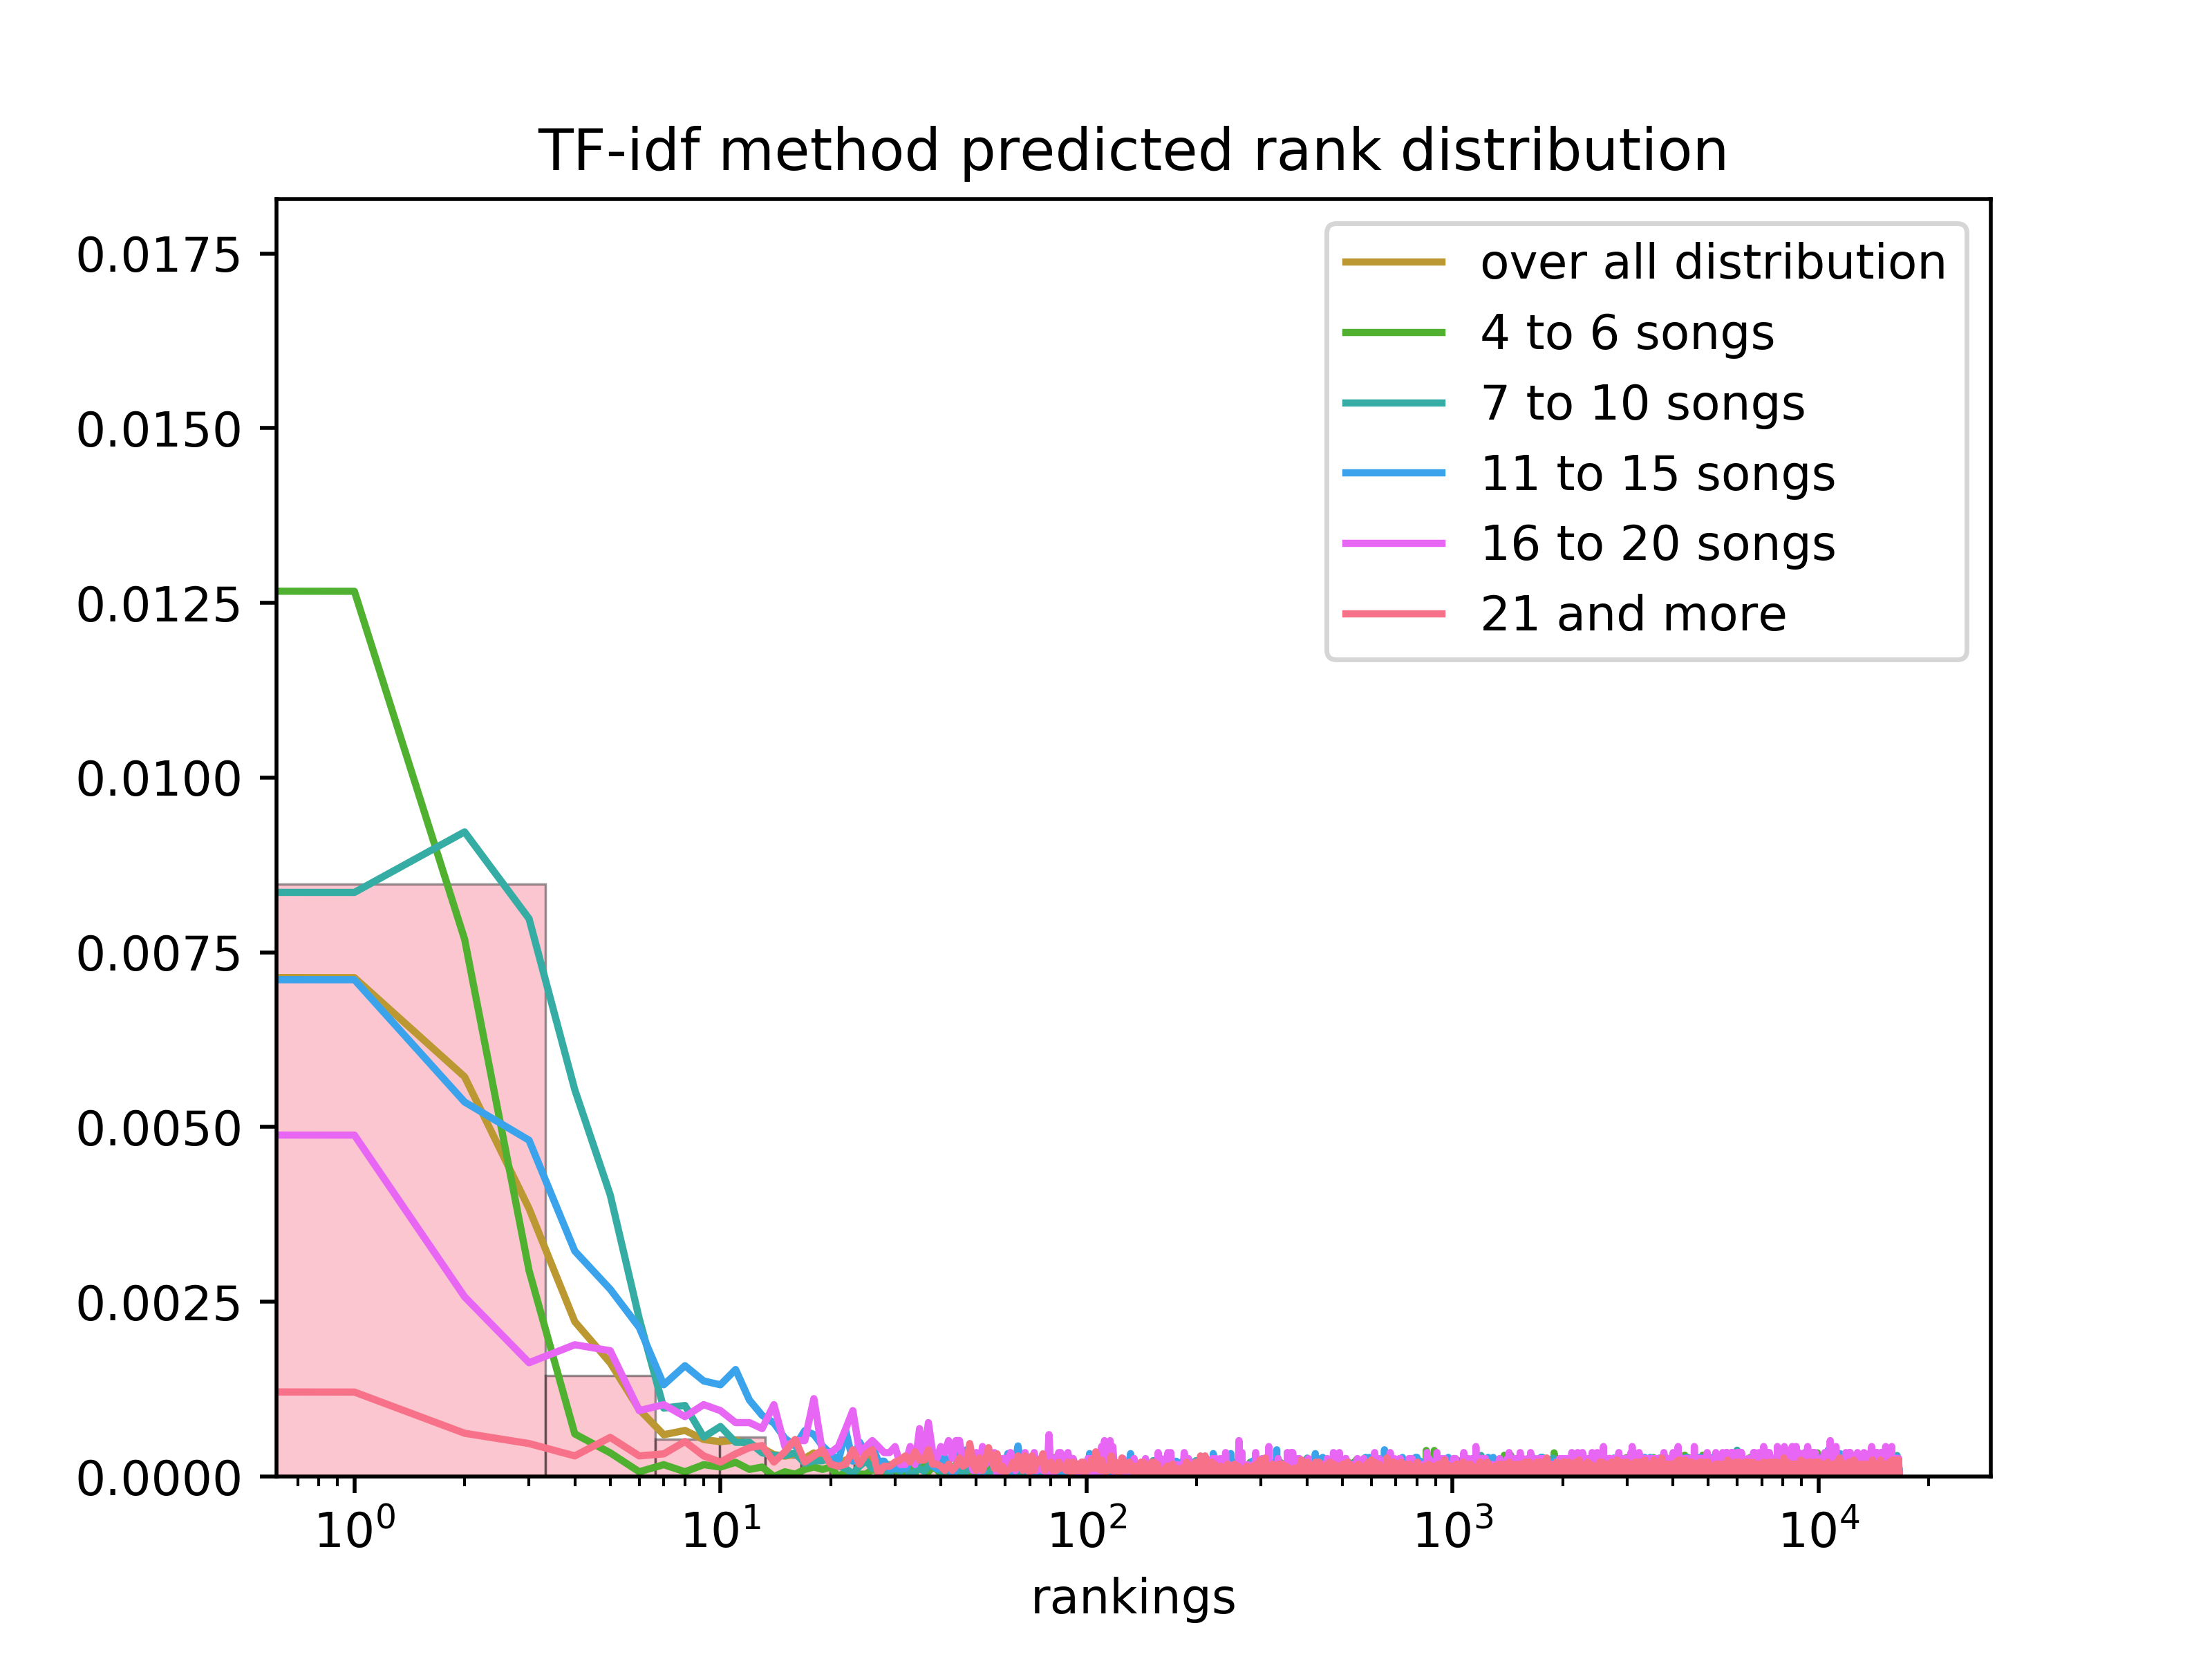
\includegraphics[width=1\linewidth]{./img/tf_idf_graph.png}
  \captionof{Distribution of ranks of songs from the $p_{test}$ set the tf-idf method assigned them.}
  \label{fig:tf_idf_distribution}
\end{minipage}%
\begin{minipage}{.5\textwidth}
  \centering
  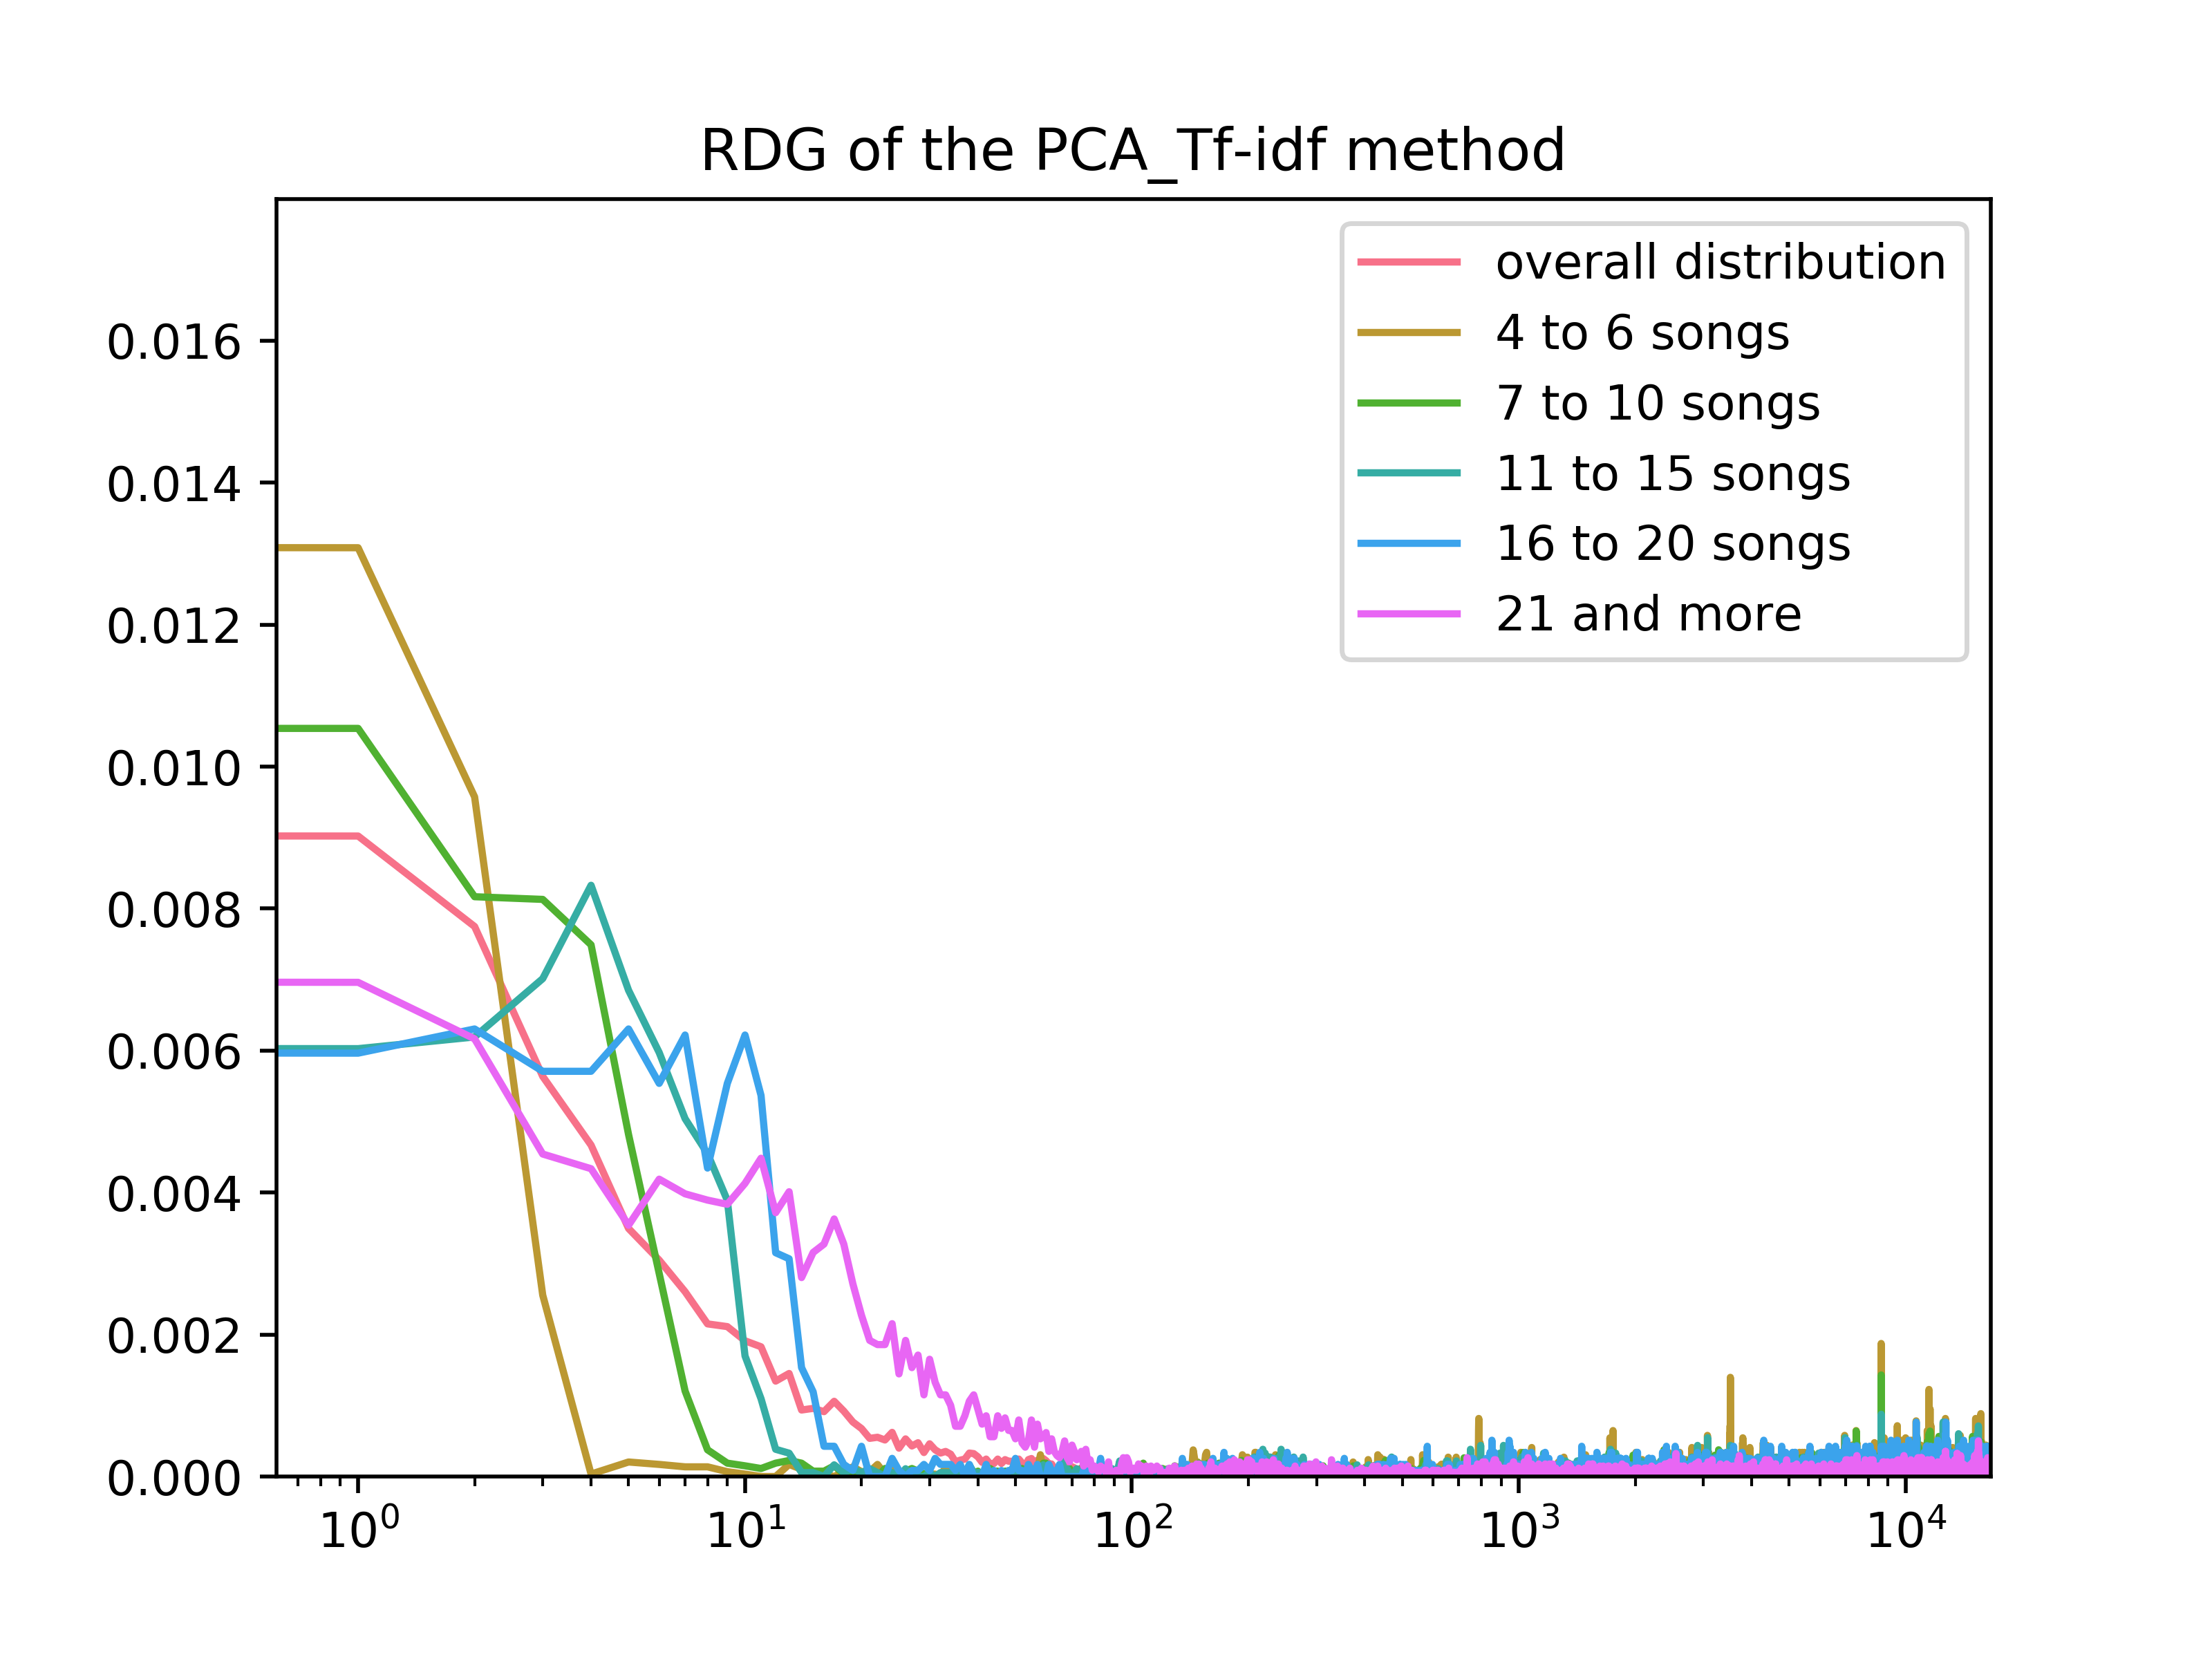
\includegraphics[width=1\linewidth]{./img/pca_tf_idf_graph.png}
  \captionof{Distribution of ranks of songs from the $p_{test}$ for tf-idf vectors as input into PCA}
  \label{fig:pca_tf_idf_distribution}
\end{minipage}
\end{figure}
\subsection{PCA on Tf-idf}\label{ssec:PCA_on_tf_idf}

Because Tf-idf has proven to yield good results we want to implement it. The long vectors pose a problem to our web application though, as it is necessary to calculate the distance between a newly added song and all the songs that are already in the database. Since the machine on which our application is running does not have such computational power as those we run our evaluations on, we decided to try to reduce the dimensions using PCA because has proven quite effective with mel spectrograms.

\subsubsection{Input}
As input, we provided the tf-idf vectors which we acquired as described \ref{ssec:TF_idf}. We did not normalize them.

\subsubsection{Training}
For training we first run a PCA from Python's \texttt{sklearn.decomposition.PCA}. We then chose the space were the explained variance ratio was equal to 90\% which left us with 4457 features. This means, our Tf-idf vector went from 40165 to 4457 dimensions. 

\subsubsection{Output}
The output were vectors of length 4457.

\subsubsection{Results}
The results of the PCA-reduced Tf-idf vector turned out to be better then those of full length. As we can see in \ref{table:1} 

\subsection{Word2Vec experiments}\label{ssec:w2v_experiments}

\subsubsection{Input}
The input for our W2V model was the same as for the Tf-idf method.

\subsubsection{Training}
In the case of Word2Vec, we did not perform any training. Instead, we used a pre-trained W2V model from Google (the first 200000 words which covered all the words in our lyric dataset). If there was a word in a song that is not in our subset added in the web application, would be ignored.

\subsubsectio{Output}
The output for a document of the Google model is a vector of fixed length 300. This is significantly lower than the Tf-idf vector.

\subsubsectio{Results}
The small size of the vectors being produced by the W2V method are a significant advantage of this method. However the results it yielded make it below average even compared to our other methods.

\begin{table}[h!]
\centering
\renewcommand{\arraystretch}{1.5}
\begin{tabu} to 1\textwidth { | c || X[c] | X[c] | X[c] | X[c] | X[c] |}
 \hline
 \textbf{method} & \textbf{R@10} & \textbf{R@50} & \textbf{R@100} & \textbf{nGDC} & $ \boldsymbol{\overline{rank}} $ \\
 \hline
 \hline
 W2V & 0.00768 & 0.01354 & 0.01983 & 0.00909 & 7682 \\
 \hline
\end{tabu} \\
\caption{Table summarizing average W2V values averaged over the 5 cross validation that were performed}
\label{table:2}
\end{table}

The table shows much lower numbers than for the Tf-idf method. Only 0.7\% of songs from the $ p_{test} $ set ranked in the top 10, 1.3\% in top 50 and 2.0\% in top 100. The average rank was 7682. That does not seem to be as bad compared to Tf-idf so it suggests that the songs did not place at the last ranks, but also not at the first ranks. \\
When looking at the distribution graph, it is very clear that the gap here between the accuracy of predicted ranks for short and longer playlists is huge. Although not great, it performs much better for short playlists. For playlists as short as 7, the performance drops significantly and it appears that for playlists with length 11 and more, the trend is opposite than what we would want, meaning, that it is more likely that a song from the $p_{test}$ set does ranks between the last 1000 than between the first 1000 if the rank is predicted based on a playlists of length at least 11.

\begin{figure}[h]
    \centering
	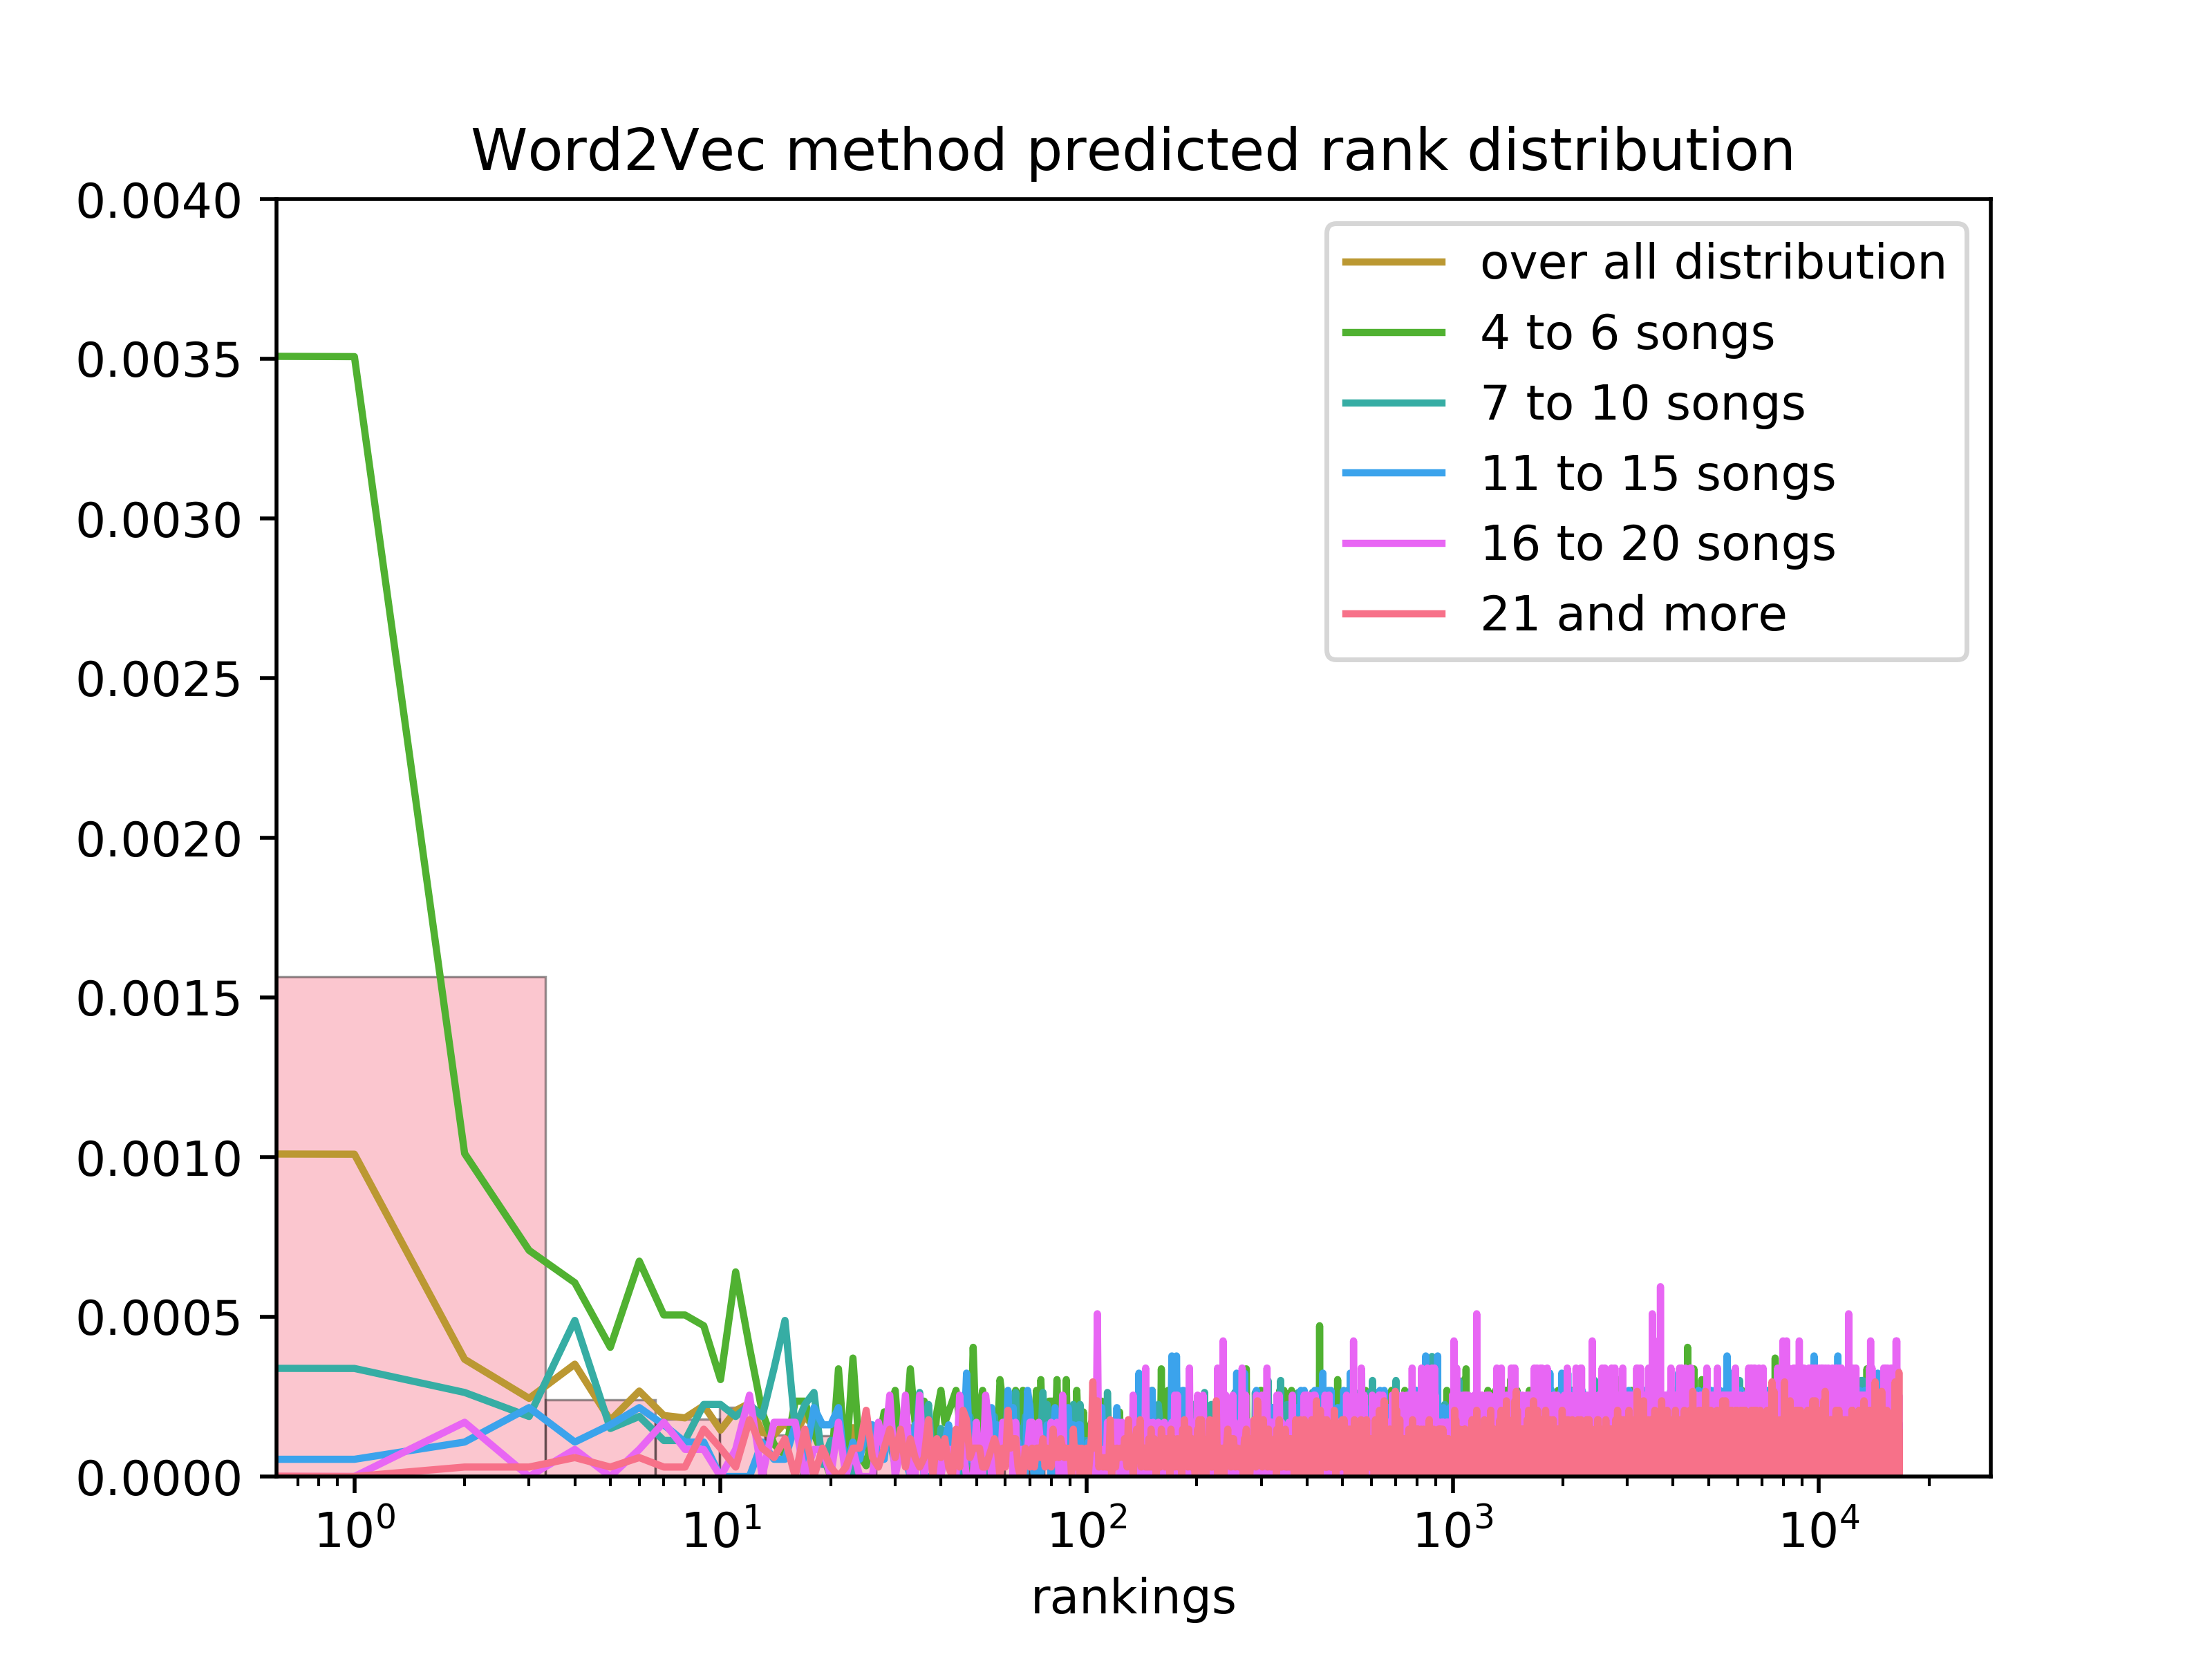
\includegraphics[width=120mm]{./img/w2v_graph.png}
	\caption{Distribution of ranks of songs from the test set the w2v method assigned them.}
	\label{fig:w2v_distribution}
\end{figure}

\subsection{SOM experiments}
We used a python library called \texttt{minisom} \cite{Vettigli2019}
\subsubsection{Input}
We tried the W2V vectors from \ref{ssec:w2v_experiments} as input for our self organizing map, mainly because of their length and also because we were hoping, that the SOM could improve the results of the W2V method. We also tried to train the SOM on the output vectors of our PCA\_Tf-idf method. We did not try the raw Tf-idf vectors as they are long and it would prolong training significantly and also, because the PCA\_Tf-idf yielded better results than raw Tf-idf.

\subsubsection{Training}
We build a self organizing map with a grid size 5 times our dataset size (16594) and the number of iterations was also 5 times our dataset size. We saved a model after each multiple of 16594 iterations and interestingly, the representations did not change after 33 187 iterations (meaning 2*16594). It was also necessary to normalize our input vectors and set learning rate to 0.2. Otherwise the songs formed 3 to 5 large clusters on the grid placing thousands of songs on the same coordinate. 
\subsubsection{Output}
The output representation for each song was a vector of length two. The whole dataset then could be displayed on a 2D map. 
When we then tried to display the map with all the songs, the size of the image would have to be immense so that all 16594 songs would be recognizable. The problem was that there were many songs to display on the map and the titles overlapped. Because of that, we decided to randomly select 20 playlists and show where the different songs that belong to each playlist placed on the map. Each playlist has its own color. This map for the W2V input is depicted in \ref{fig:som_map}. Obviously, the playlists do not really form any visible clusters.
\begin{figure}[h]
    \centering
	\includegraphics[width=140mm]{./img/som_map.png}
	\caption{The location of different songs from 20 randomly selected playlists on the map created by SOM. Each playlist has its own colour.}
	\label{fig:som_map}
\end{figure}
\subsubsection{Results}
The fact that the playlists do not form clusters is also supported by the fact that the overall results for the self organizing map algorithm are quite poor. Actually it is the worse method that we implemented and our hope to improve the results of W2V were not fulfilled.

\begin{table}[h!]
\centering
\renewcommand{\arraystretch}{1.5}
\begin{tabu} to 1\textwidth { | c || X[c] | X[c] | X[c] | X[c] | X[c] |}
 \hline
 \textbf{method} & \textbf{R@10} & \textbf{R@50} & \textbf{R@100} & \textbf{nGDC} & $ \boldsymbol{\overline{rank}} $ \\
 \hline
 \hline
 SOM with W2V & 0.00084 & 0.0038 & 0.00664 & 0.00192 & 8152 \\
 \hline
 SOM wiht PCA_Tf-idf & 0.000435 & 0.002084 & 0.004621 & 0.001254 & 8243 \\
 \hline
\end{tabu} \\
\caption{Table summarizing average SOM values averaged over the 5 cross validations}
\label{table:som}
\end{table}
The distribution graph of the SOM\_W2V method clearly shows, that the distribution of ranks is random or worse which is also suggested by the fact that the average rank is 8152 which almost in the middle of 16594. The main reason for the failure of this method is unclear but it is possible that the data from the W2V vectors that already contain too little information for the SOM network to be able to cluster data based on it.  But since we recieved even worse results for the SOM\_Tf-id we are more inclined to another possibility which is, that the SOM network is not be able to provide satisfying results because two dimensions are simply too little to represent the whole complexity of the input data.
\begin{figure}[h]
    \centering
	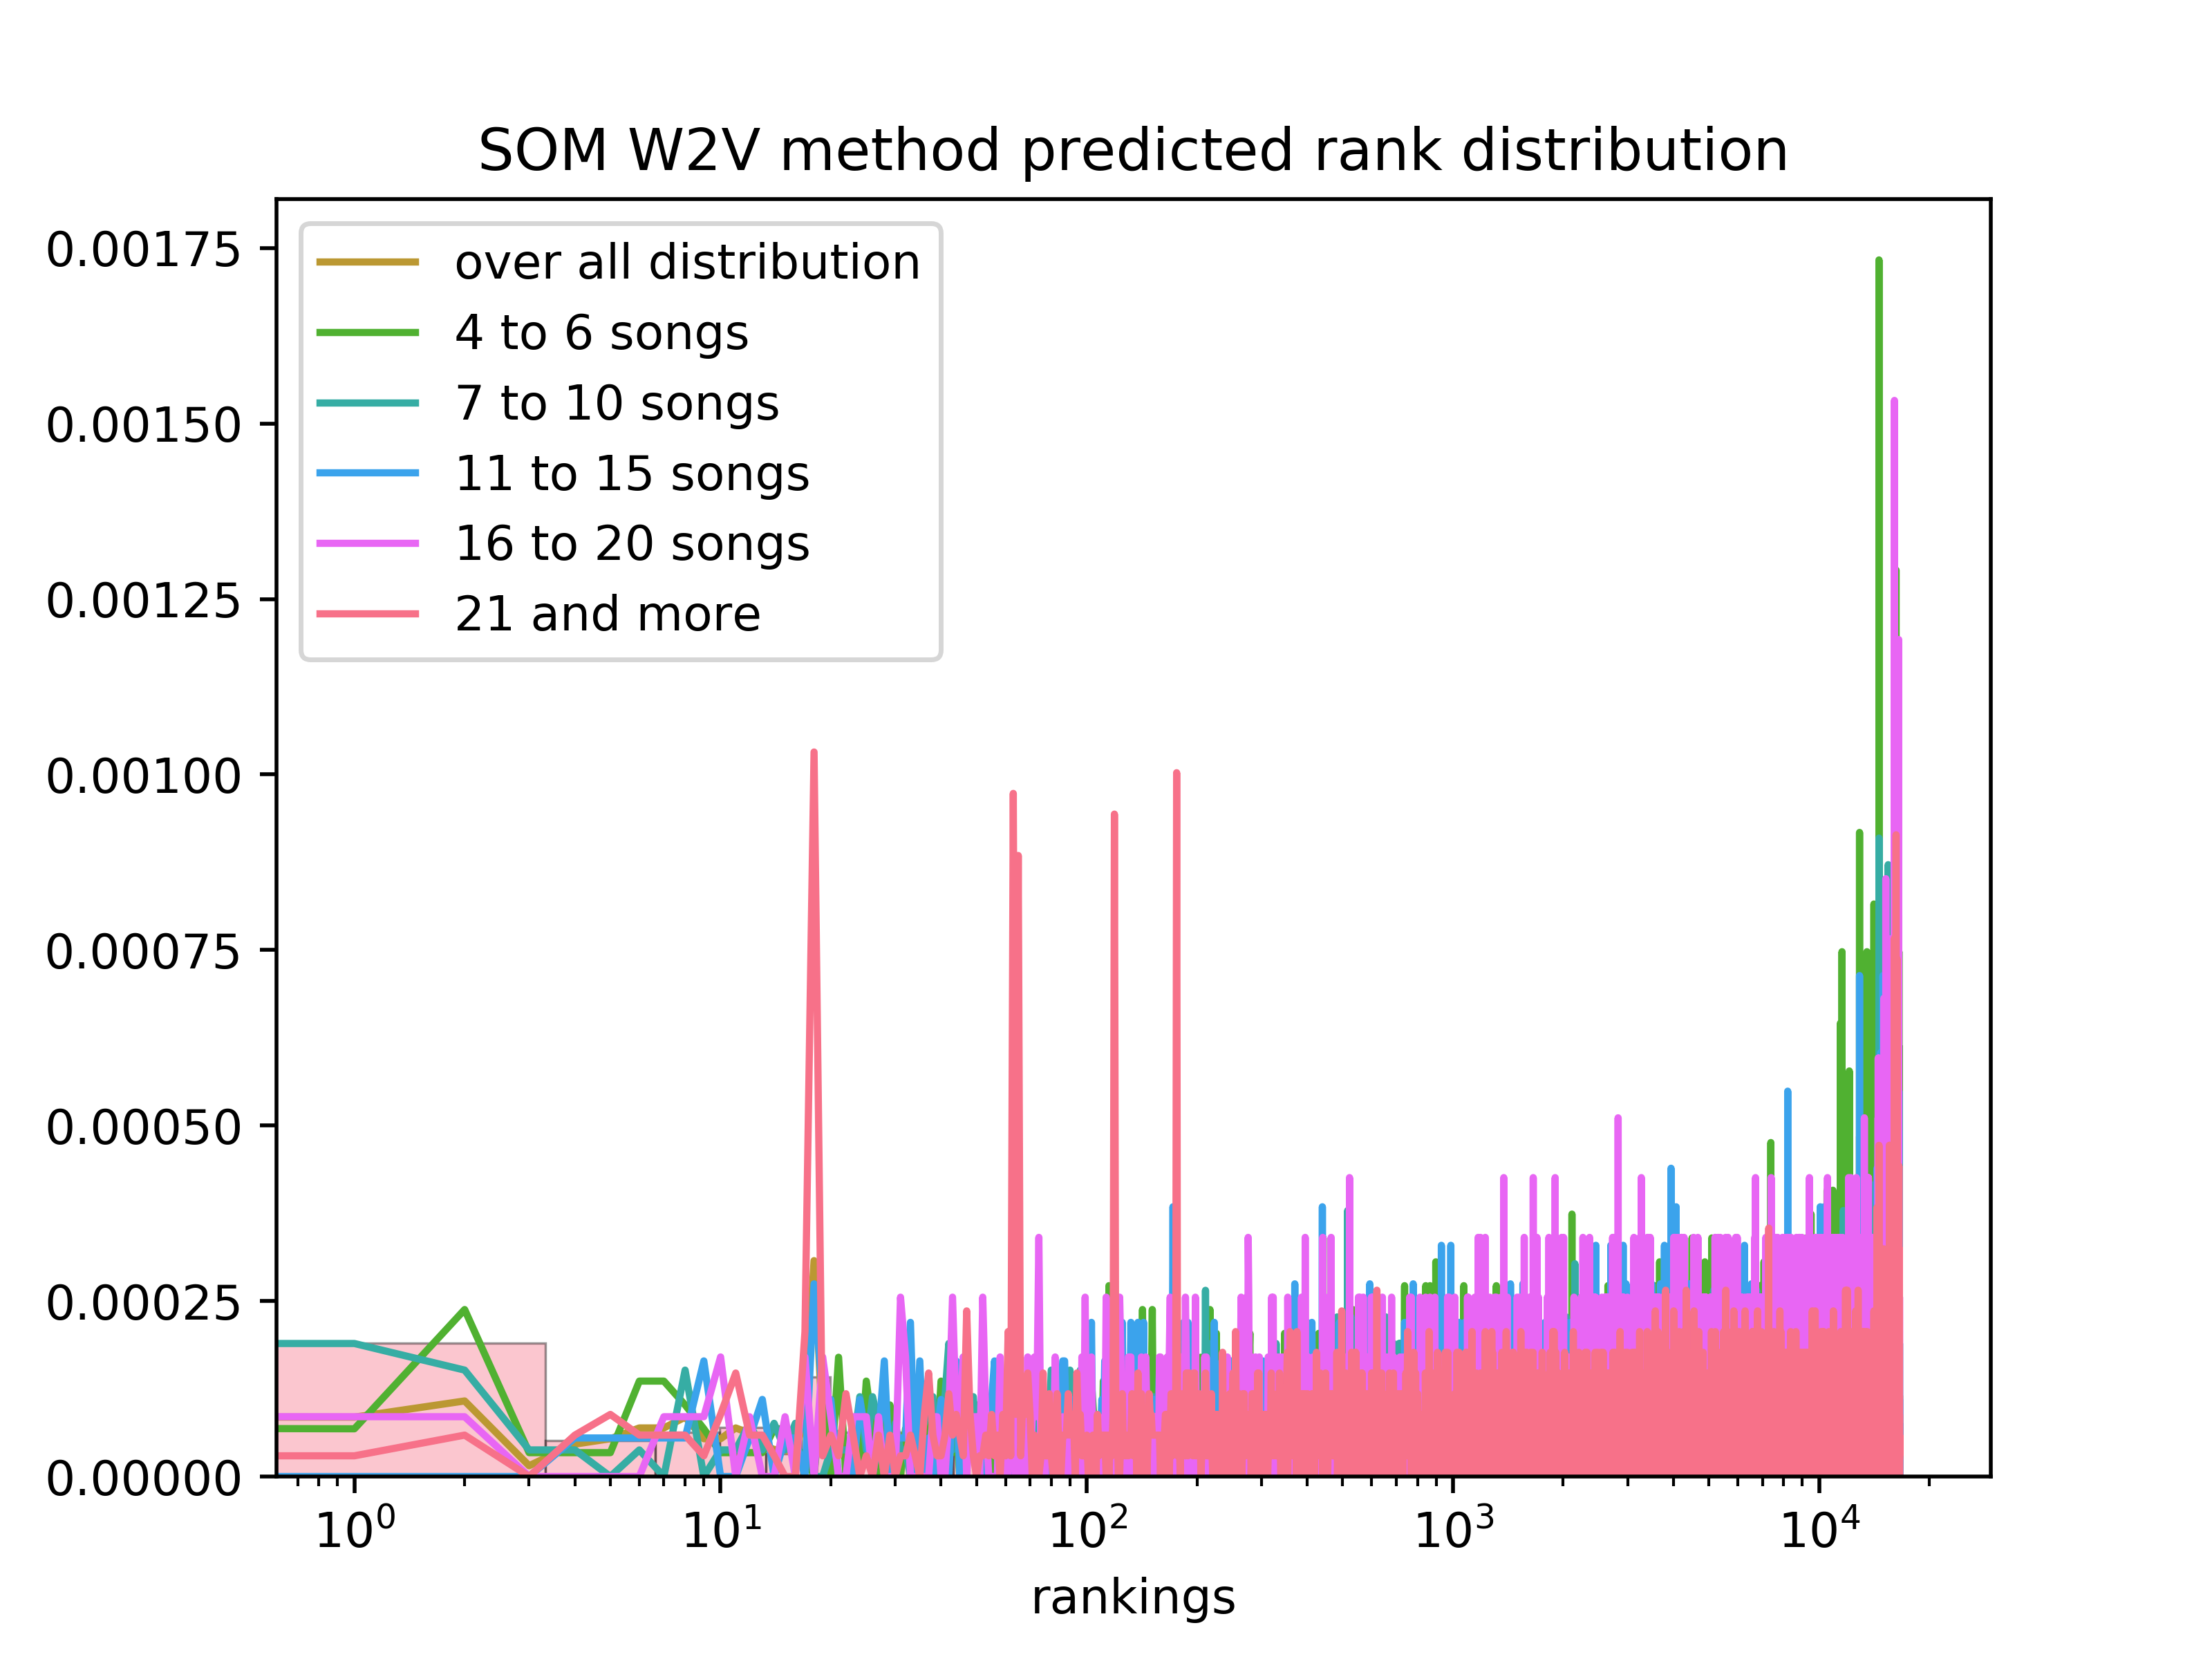
\includegraphics[width=120mm]{./img/som_w2v_graph.png}
	\caption{Distribution of ranks of songs from the test set the SOM method assigned them.}
	\label{fig:som_distribution}
\end{figure}
\section{Simple audio method experiments}
\subsection{Audio preparation}\label{ssec:audio_prep}

In order to encode audios of songs, we first needed to acquire some form of the music to become our standard. To make our audio information suitable for machine learning, we decided to extract audios of the same length so our vectors (spectrograms, mel-spectrograms and mfccs are also of the same length). Since all songs have different lengths and also, one complete 3.5 minute long song results in a spectrogram of size 5214x2206 which when flattened is a vector of length 11 502 084. Therefore we decided to extract 15 second excerpts from each song to create spectrograms, mel-spectrograms and MFCCs from those. We took 5 seconds between the 15th and 20th second, 5 seconds starting in the middle of the song and 5 second starting 15 seconds before the end. We did not start at the beginning and the end because in some songs, there is silence or applause or some talking before the actual song starts. \\

It was also necessary to decide on some parameters for spectrograms, mel-spectrograms and MFCCs. As stated previously, our neural networks were inspired by \cite{inproceedings_RNNs} where they also performed parameter optimisation. We decided to use their parameters as input for all our methods. It is possible that some parameters values suite some methods better than others but because of the amount of methods we tested we decided it would too difficult to optimise them for each method. We also think, that it a good idea to have all methods work with more or less the same input as their comparison is less ambiguous. \\
The resulting choices were following. We set window width $w$ to 0.2 and window overlap $w_o$ to 0.5$w$ = 0.1. For mel-spectrograms it is also necessary to choose Mel frequency bands which was set to 320 as for values above 320, the performance of neural networks did not increase. For MFCC coefficients we decided to set the number of MFCC coefficients to 320 which is the same as the number of Mel frequency bands.

We used Python's \texttt{librosa} library \cite{brian_mcfee_2019_2564164} to cut our songs and to generate our spectrograms, mel spectrograms and MFCCS using functions \texttt{librosa.core.stft} for spectrograms \texttt{librosa.feature.mel\_spectrogram} for mel-spectrograms and \texttt{librosa.feature.mfcc} for MFC coeficients. The audio data for training was stored in .wav files.

\subsection{Raw Mel spectrograms}\label{ssec:raw_mels}
The input for mel spectrograms was the 15 second long audio described in \ref{ssec:audio_prep}. Extracting spectrograms does not require any training. It a is mathematical procedure explained in \ref{ssec:mel_spectrograms_intro}.

The mel-spectrograms we got after transforming a 15 second long audio with 320 Mel frequencies bands was a matrix of size 408x320 which when flattened is a vector of size 130560. This turned out to be too long to implement in our application, however because we did not realize that at first, we tested this method and got the following results. \\
As can be seen in \ref{table:mel_spec_methods} 3.7\% of songs ended up between top ten predictions, 4.3\% in top 50 and 4.7\% in the top 100. These results are actually better than any other method using mel-spectrograms as input except of PCA. It beats both neural network architectures with mel-spectrogram input. 

\subsubsectio{Results}
\begin{table}[h!]
\centering
\renewcommand{\arraystretch}{1.5}
\begin{tabu} to 1\textwidth { | c || c | c | c | c | c |}
 \hline
 \textbf{method} & \textbf{R@10} & \textbf{R@50} & \textbf{R@100} & \textbf{nGDC} & $ \boldsymbol{\overline{rank}} $ \\
 \hline
 \hline
 Raw mel spectrograms & 0.03696 & 0.04275 & 0.0473 & 0.03063 & 7604 \\
 \hline
 PCA_mel_5715 & 0.05243 & 0.06153 & 0.06737 & 0.04300 & 6851 \\
 \hline
 PCA_mel_320 & 0.00053 & 0.00196 & 0.00633 & 0.00155 & 8357 \\
 \hline
 GRU_mel  & 0.03623 & 0.04336 & 0.04870 & 0.03119 & 7601 \\
 \hline
 LSTM_mel & 0.01368 & 0.02028 & 0.02579 & 0.01423 & 7861\\
 \hline
\end{tabu} \\
\caption{Table summarizing average rank values for all methods with mel-spectrogram input averaged over the 5 cross validations}
\label{table:mel_spec_methods}
\end{table}
  
The patterns observed in \ref{fig:mel_graph} which shows the distribution of ranks for raw mel-spectrograms is similar to all other methods we are studying (except of those that appear to be random such as SOM). The ranking is better when predicting ranks of songs from shorter playlists. 

\begin{figure}[h]
    \centering
	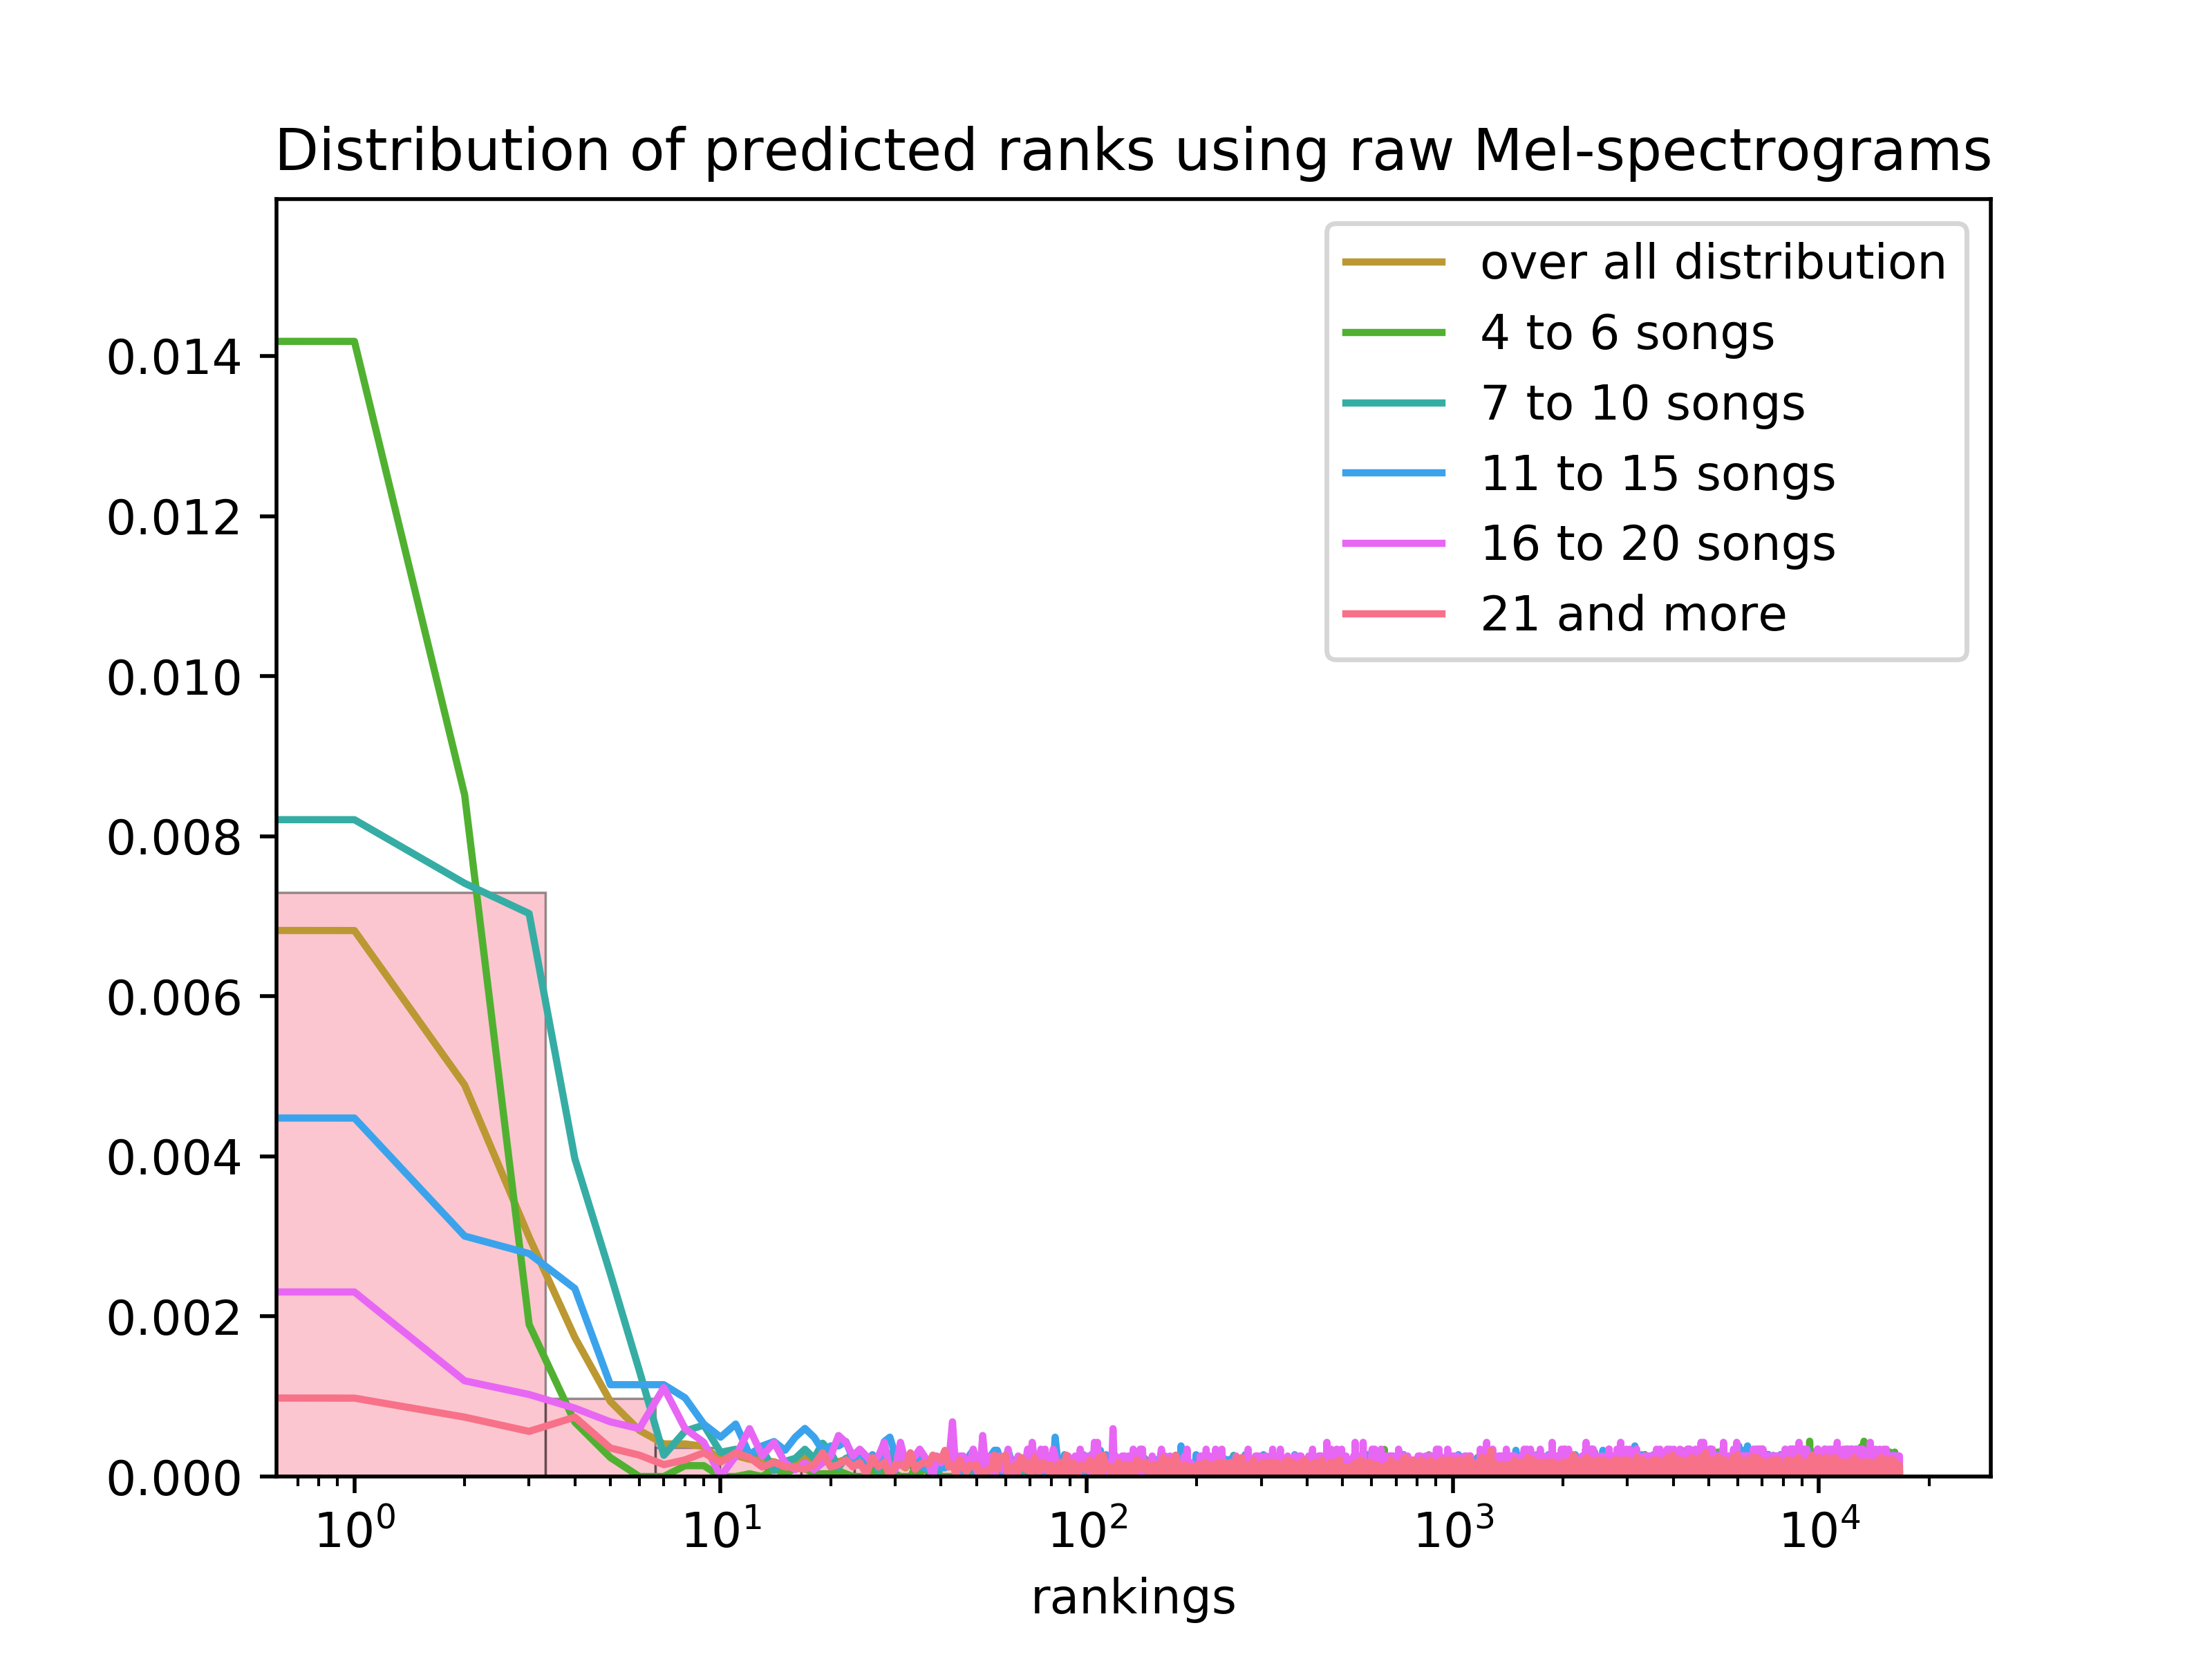
\includegraphics[width=120mm]{./img/mel_graph.png}
	\caption{Distribution of ranks of songs from the test with their similairity defined as cosine distance between mel-spectrograms.}
	\label{fig:mel_graph}
\end{figure}

\subsection{Raw MFCCs}
Our 15 second audios were fed as input into the texttt{librosa.feature.mfcc()} function with parameters mentioned in \ref{ssec:audio_prep}. Training was not necessary since acquiring mel-frequency cepstral coefficient is a matter of Fourier Transformations and the resulting matrix had the shape of 646x128. When flattened we get a vector of length 82866. This has proven to be too long for practical use in our application, however we still have the evaluation results when defining song similarity as the cosine distance between flattened MFCC matrices.

\subsubsection{Results}

The results of MFCCs are quite poor even compared to our other methods. Only 0.4\% of songs missing in our playlists rank betwen the top 10, 0.9\% in the top 50 and 1.4\% in the top 100. However as can be seen in table \ref{table:mfcc_methods} it is better than when using mfc coefficients with our LSTM network.
\begin{table}[h!]
\centering
\renewcommand{\arraystretch}{1.5}
\begin{tabu} to 1\textwidth { | c || X[c] | X[c] | c | X[c] | X[c] |}
 \hline
 \textbf{method} & \textbf{R@10} & \textbf{R@50} & \textbf{R@100} & \textbf{nGDC} & $ \boldsymbol{\overline{rank}} $ \\
 \hline
 \hline
 Raw MFCC & 0.00415 & 0.00919 & 0.01423 & 0.00607 &  7552 \\
 \hline
 LSTM\_MFCC & 0.00246 & 0.00674 & 0.0116 & 0.00436 & 7665 \\
 \hline
 GRU\_MFCC & 0.00510 & 0.01148 & 0.01755 & 0.00721 & 7391 \\
 \hline
\end{tabu} \\

\caption{Table summarizing average rank values for all methods with MFCC input averaged over the 5 cross validations}
\label{table:mfcc_methods}
\end{table}

 When looking at our traditional distribution graph, we again observe the a lower probability of good song rankings as the length of playlists increases. Again completely against what we hope for. 
\begin{figure}[h]
    \centering
	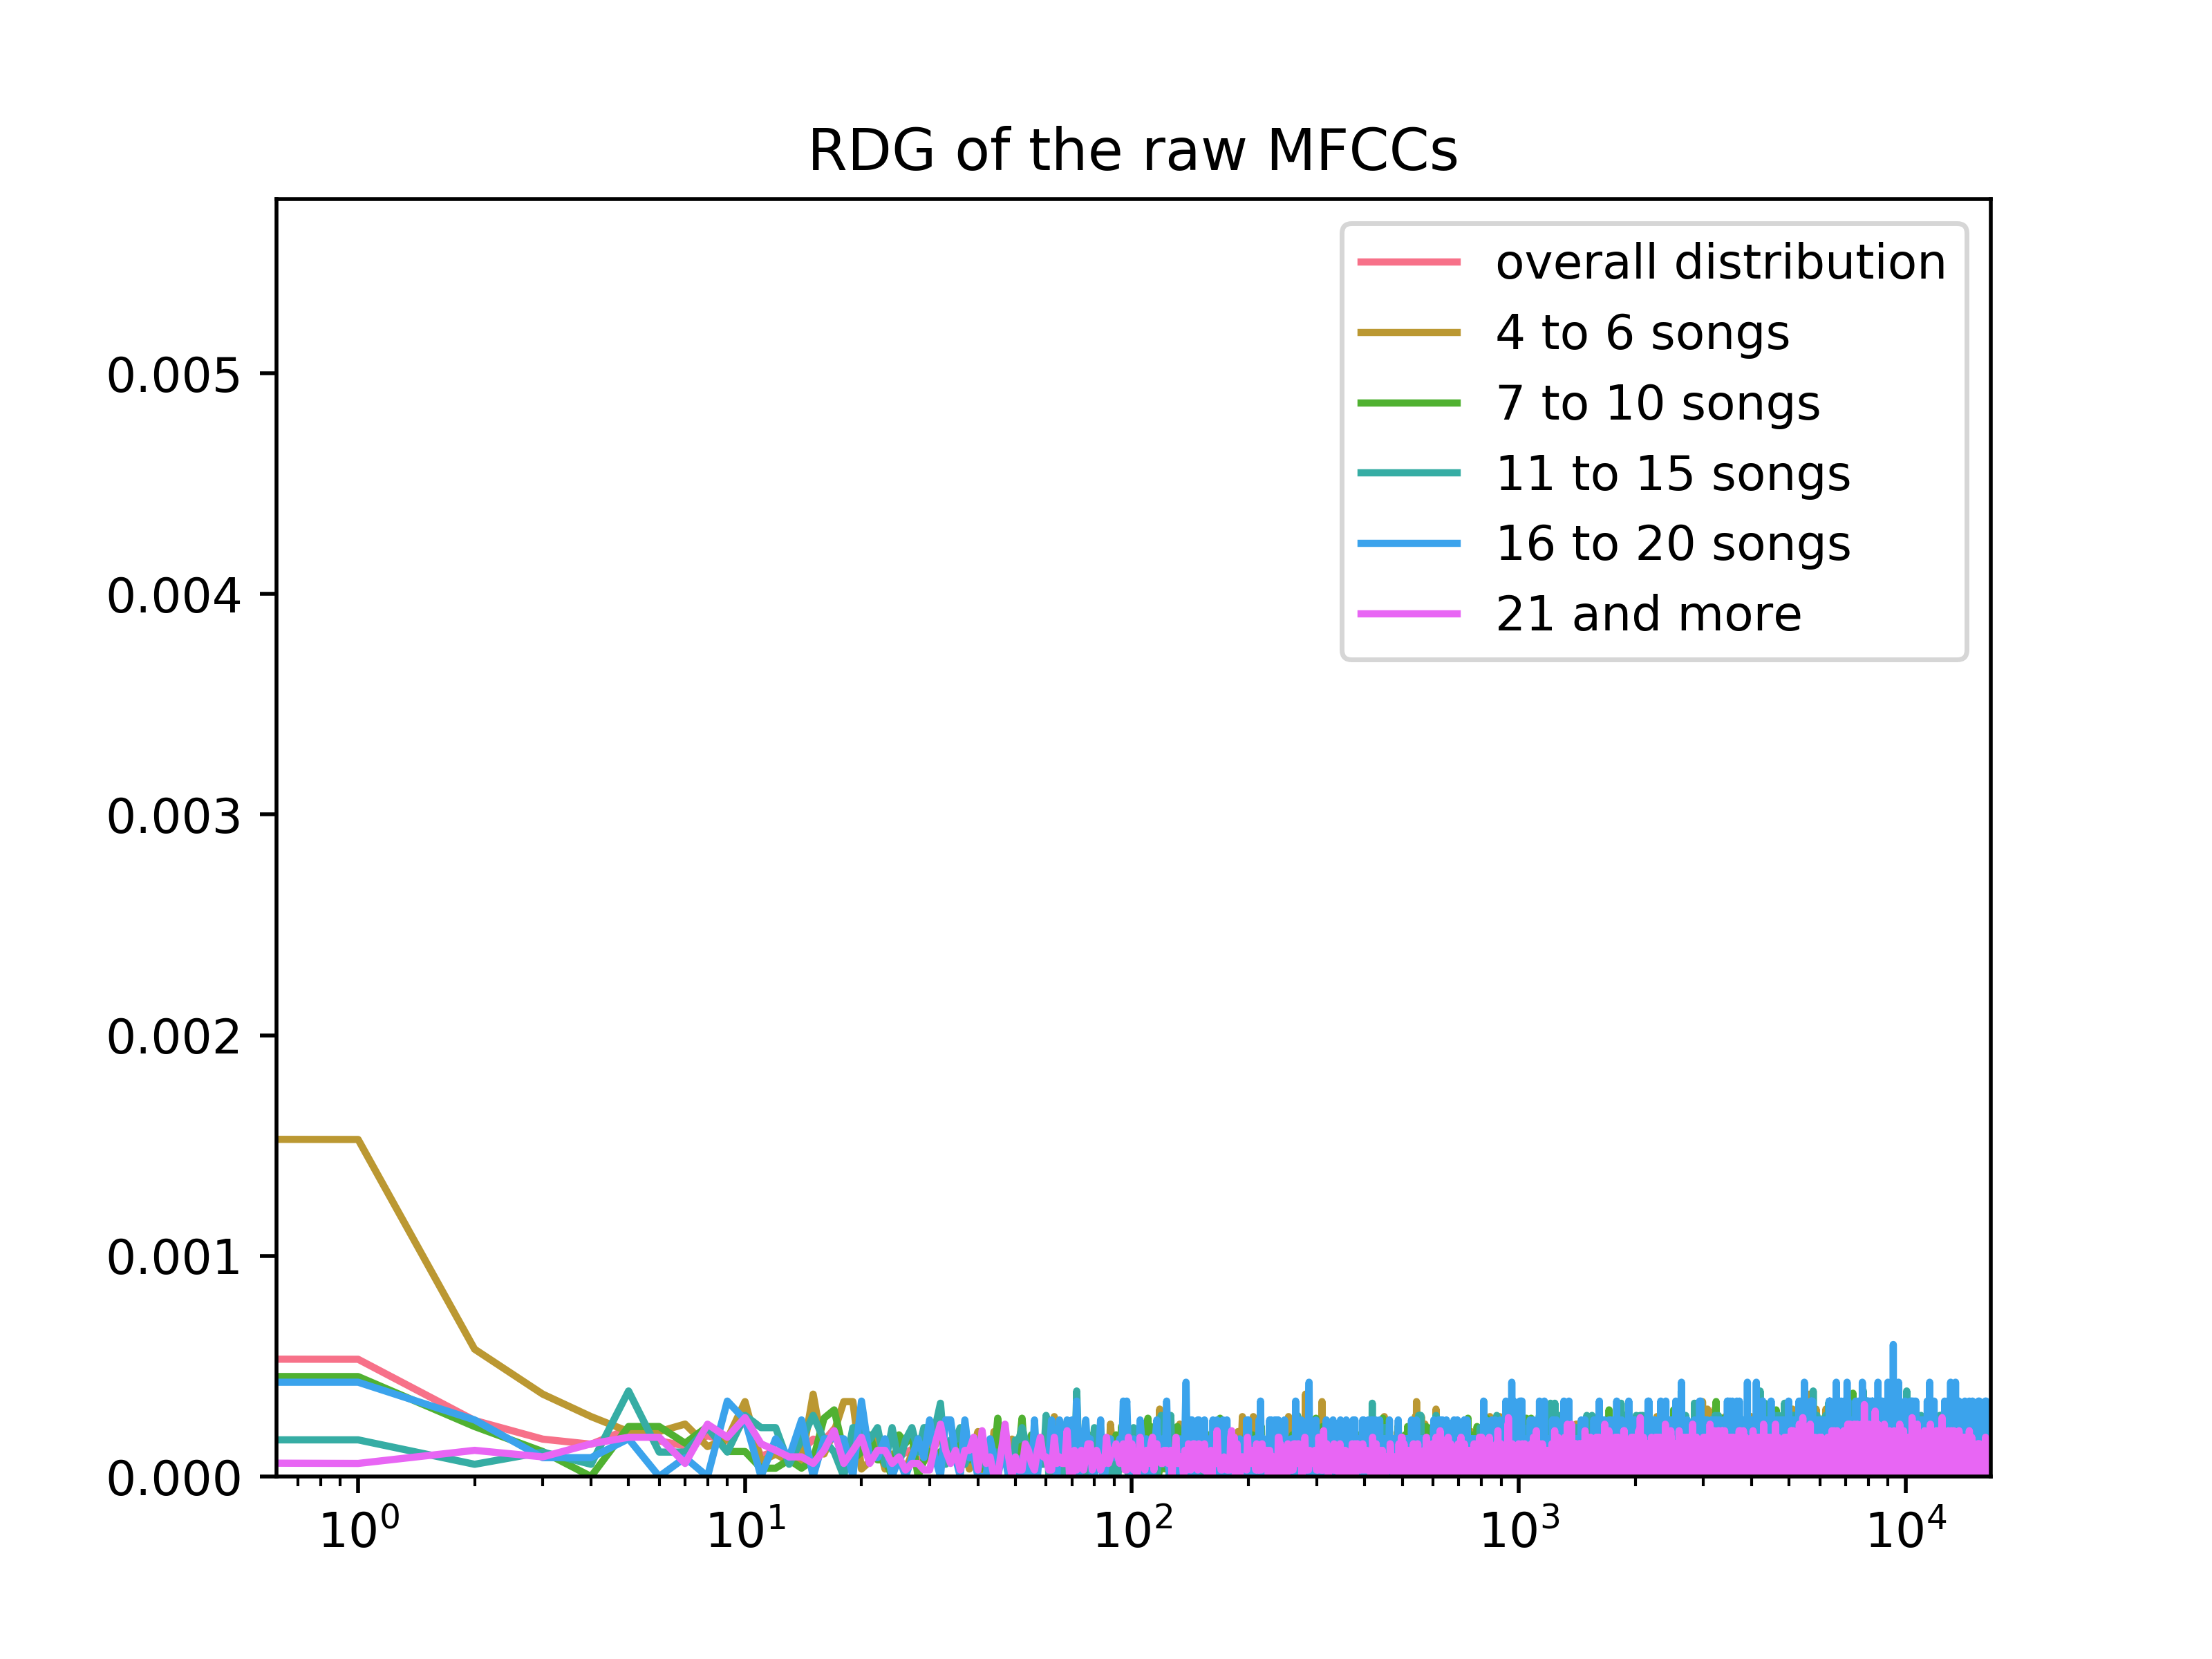
\includegraphics[width=120mm]{./img/mfcc_graph.png}
	\caption{Distribution of ranks of songs from the test set the MFCC method assigned them.}
	\label{fig:mfcc_graph}
\end{figure}


\subsection {PCA on spectrograms}

\subsubsection{Input}
We used spectrograms as described in \ref{ssec:audio_prep} as input for our PCA. Because the output of the \texttt{librosa.core.stft()} method is a complex matrix, we computed the absolute value for each matrix entry. Afterwards, we flattened the matrix into a single vector and normalized it. Normalization was very important, without it, the resulting rankings were almost random.

\subsubsection{Training}
Training proved to be a little bit challenging with input vectors of length 900048. As the whole (16594x900048) matrix did not fit into the PCA at once. So instead of using \texttt{sklearn.decomposition.PCA} we turned to a PCA with the possibility to train the PCA in batches. This kind of PCA is also provided by \textt{skearn} in the \texttt{sklearn.decomposition.incrementalPCA} module. \\ Our batch size was 1106. Again, when we tried to increase it, we got a memory error. This was a little inconvenient as for the PCA the maximum number of components is $min(n\_samples, n\_features)$. In our case, $n\_samples$ was only 1106 components which explained about 57\% of the dataset's variance.

\subsubsectio{Output}
Our output were vectors of length 1106 which we acquired when taking the trained incremental PCA model and calling \texttt{tranform()} with the spectrogram as a parameter.

\subsubsection{Results}

\begin{table}[h!]
\centering
\renewcommand{\arraystretch}{1.5}
\begin{tabu} to 1\textwidth { | c || c | c | c | c | c |}
 \hline
 \textbf{method} & \textbf{R@10} & \textbf{R@50} & \textbf{R@100} & \textbf{nGDC} & $ \boldsymbol{\overline{rank}} $ \\
 \hline
 \hline
 PCA\_spec\_1106 & 0.04317 & 0.05213 &  0.05945 & 0.03741 & 6729 \\
 \hline
 PCA\_spec\_320 & 0.03373 & 0.04392 &  0.05189 & 0.03209 & 6768 \\
 \hline
 GRU\_spec\_20400 & 0.00214 & 0.00563 & 0.00999 & 0.00356 & 7710 \\
 \hline
 GRU\_spec\_5712 & 0.00219 & 0.00616 & 0.01017 & 0.00370 & 7667 \\
 \hline
 LSTM\_spec\_20400 & 0.00924 & 0.01595 & 0.02214 & 0.01060 & 7601 \\
 \hline
 LSTM\_spec\_5712 & 0.00619 & 0.01244 & 0.01737 &  0.00744 & 7452 \\
 \hline
\end{tabu} \\
\caption{Table summarizing average rank values for all methods with spectrogram input averaged over the 5 cross validations}
\label{table:spec_methods}
\end{table}
 

\begin{figure}[h!]
\centering
\begin{minipage}{.5\textwidth}
  \centering
  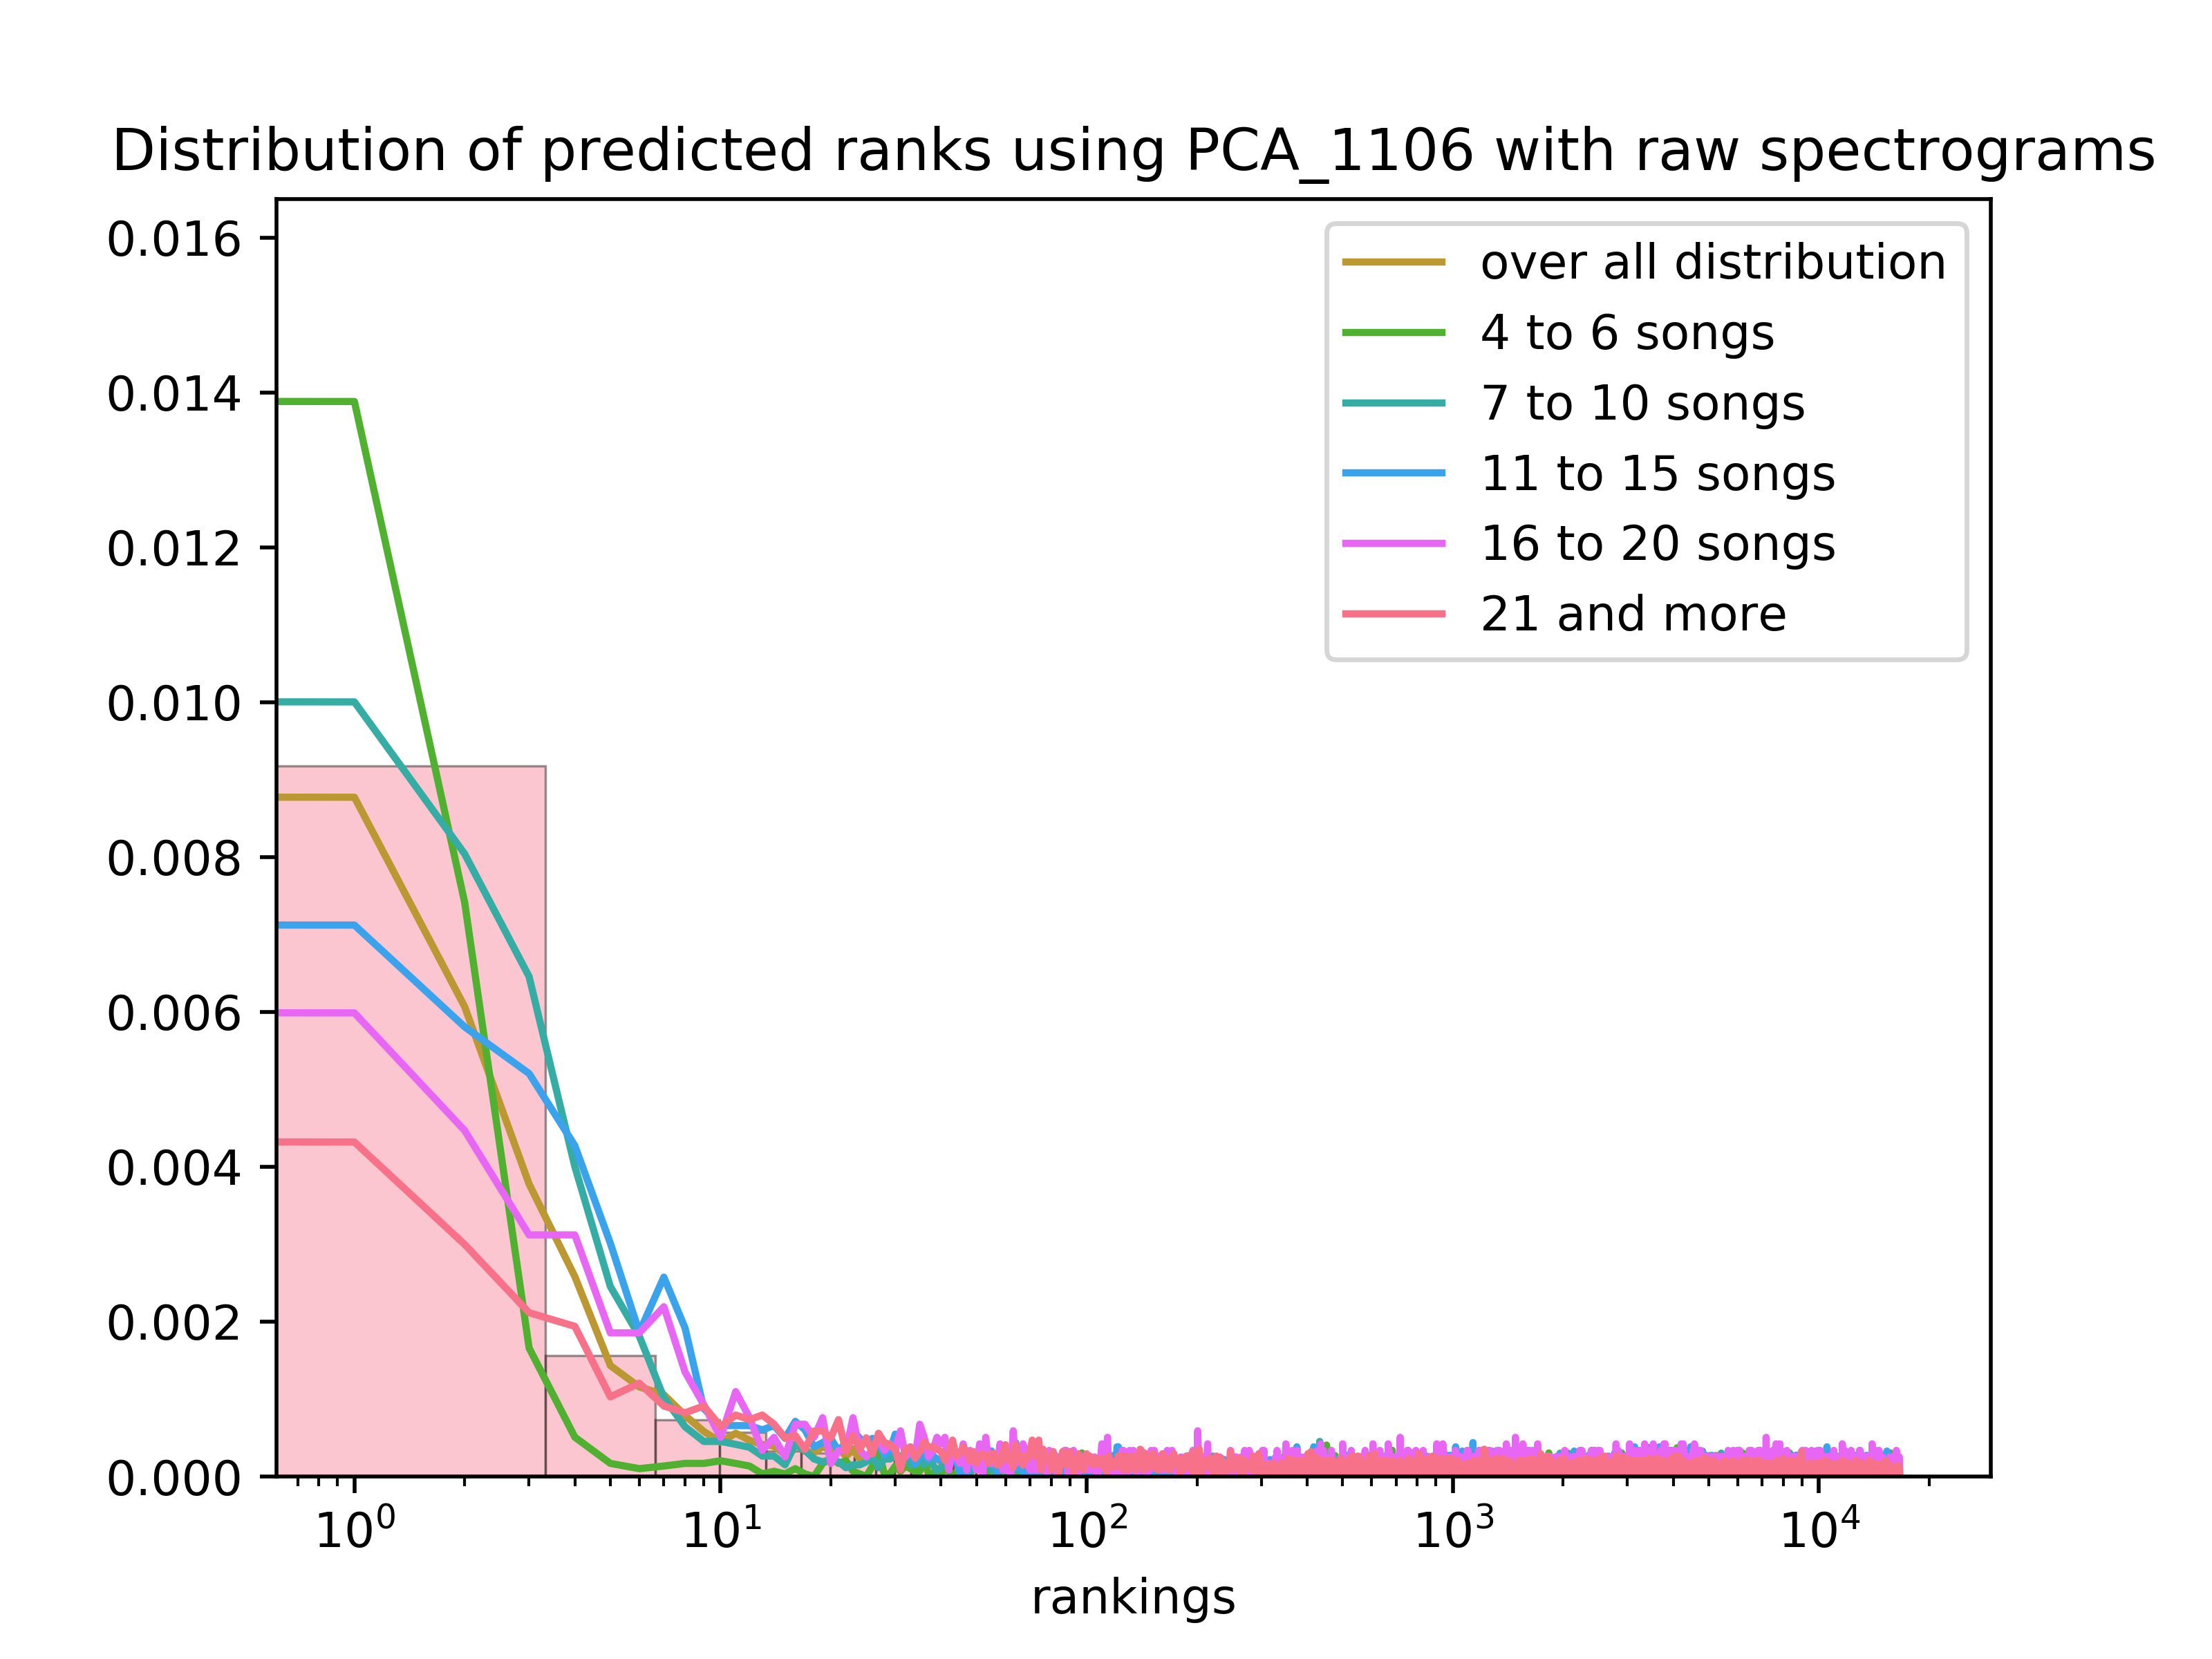
\includegraphics[width=1\linewidth]{./img/pca_spec_1106_graph.png}
  \captionof{Distribution of ranks of songs from the $p_{test}$ set the spectrograms method assigned them.}
  \label{fig:pca_spec_1106_distribution}
\end{minipage}%
\begin{minipage}{.5\textwidth}
  \centering
  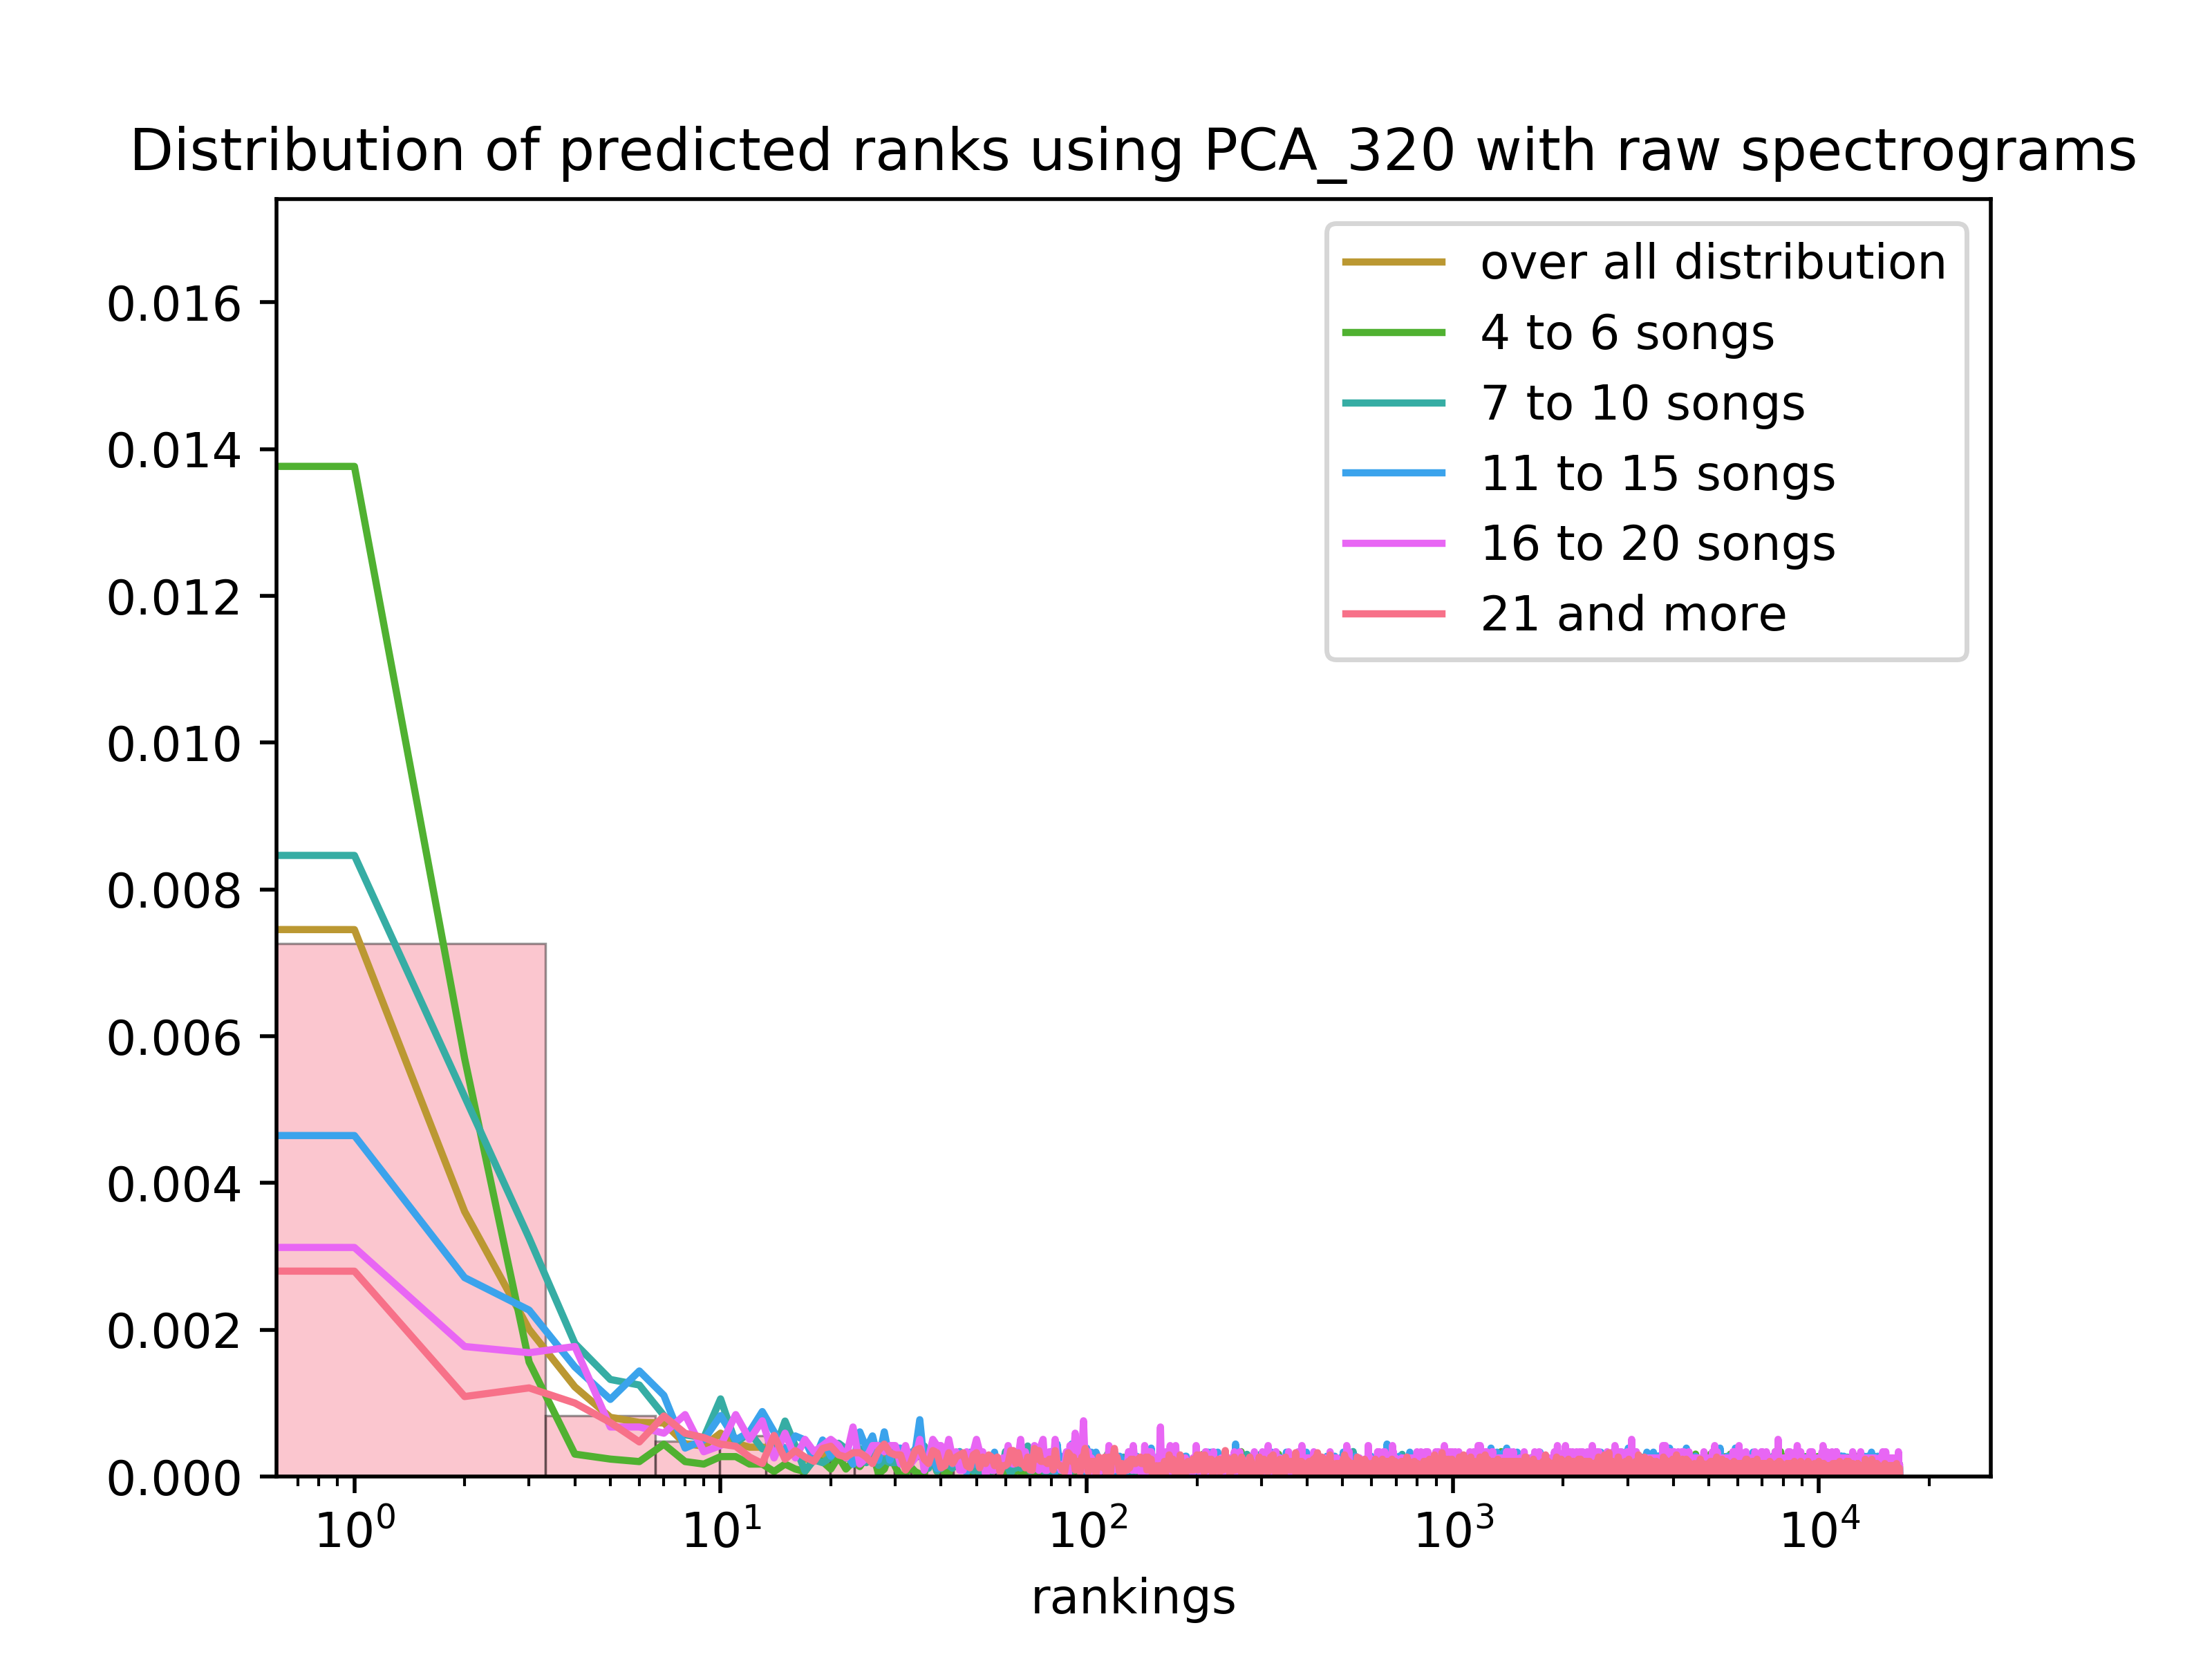
\includegraphics[width=1\linewidth]{./img/pca_spec_320_graph.png}
  \captionof{Distribution of ranks of songs from the $p_{test}$ for spectrograms vectors as input into PCA}
  \label{fig:pca_spec_320_distribution}
\end{minipage}
\end{figure}

The dimensionality reduction in this method was the biggest of all or our methods. Our song representation went from 900048 to 1106 dimensions. It seems though that even with only 57\% of explained variance this methods results were very good compared to other methods. \\
When seeing this, we decided to go for a even more radical reduction to vectors of length 320. This was inspired by the length of the W2V vectors. We called our bigger model $PCA_{1106}$ and our smaller model $PCA_{320}. $ The results of the smaller model were only slightly worse than those of the big one. This is especially interesting because the same tendencies were not observed in the case of PCAs with Mel-spectrogram inputs as will be illustrated later.

\subsection{PCA with Mel-spectrograms}
\subsubsection{Input}
The input for our Mel-PCA were mel-spectrograms from \ref{ssec:audio_prep} which were flattened and normalized using a \texttt{MinMaxScaler} from the \texttt{sklearn} Python package.

\subsubsection{Training}
Unlike with the spectrograms, mel-spectrograms fit into the memory so the PCA was able to train with the whole dataset at once. This allowed us again to find out what number of components explaines 90\% of the variance ratio and to use it. We found that 90\% of variance is explained by 5715 components which is also what we used to train our first model. \\
We were quite pleased by the results as it is the best method that we came up with. Therefore we were quite hopeful when reducing the dimension even more to 320 as we did with PCA on spectrograms. We again created two models, one is called the $Mel\_PCA_{5715}$ the other the $Mel\_PCA_{320}$. 

\subsubsection{Output}
Our output for the bigger model was a vector of length 5715, for the smaller model, it was a vector of length 320.

\subsubsection{Results}
To our disappointment, the more radical dimension reduction did not improve the performance of the PCA\_mel method. It actually worsened the results significantly as can be observed in Table \ref{table:mel_spec_methods}. 

The \ref{fig:pca_mel_comparison_graps} illustrates the immense performance drop between a PCA\_mel\_5715 components and a PCA\_mel\_320. Another thing to notice here though which only applies to the Mel\_PCA\_{5715} is that the drop of top rankings for longer playlists is not quite significant compared to all the other methods we tested. We still observe the trend of worse results for longer playlists, however, it is not as significant compared to for example the the method with raw Mel-spectrograms.
\begin{figure}[h!]
\centering
\begin{minipage}{.5\textwidth}
  \centering
  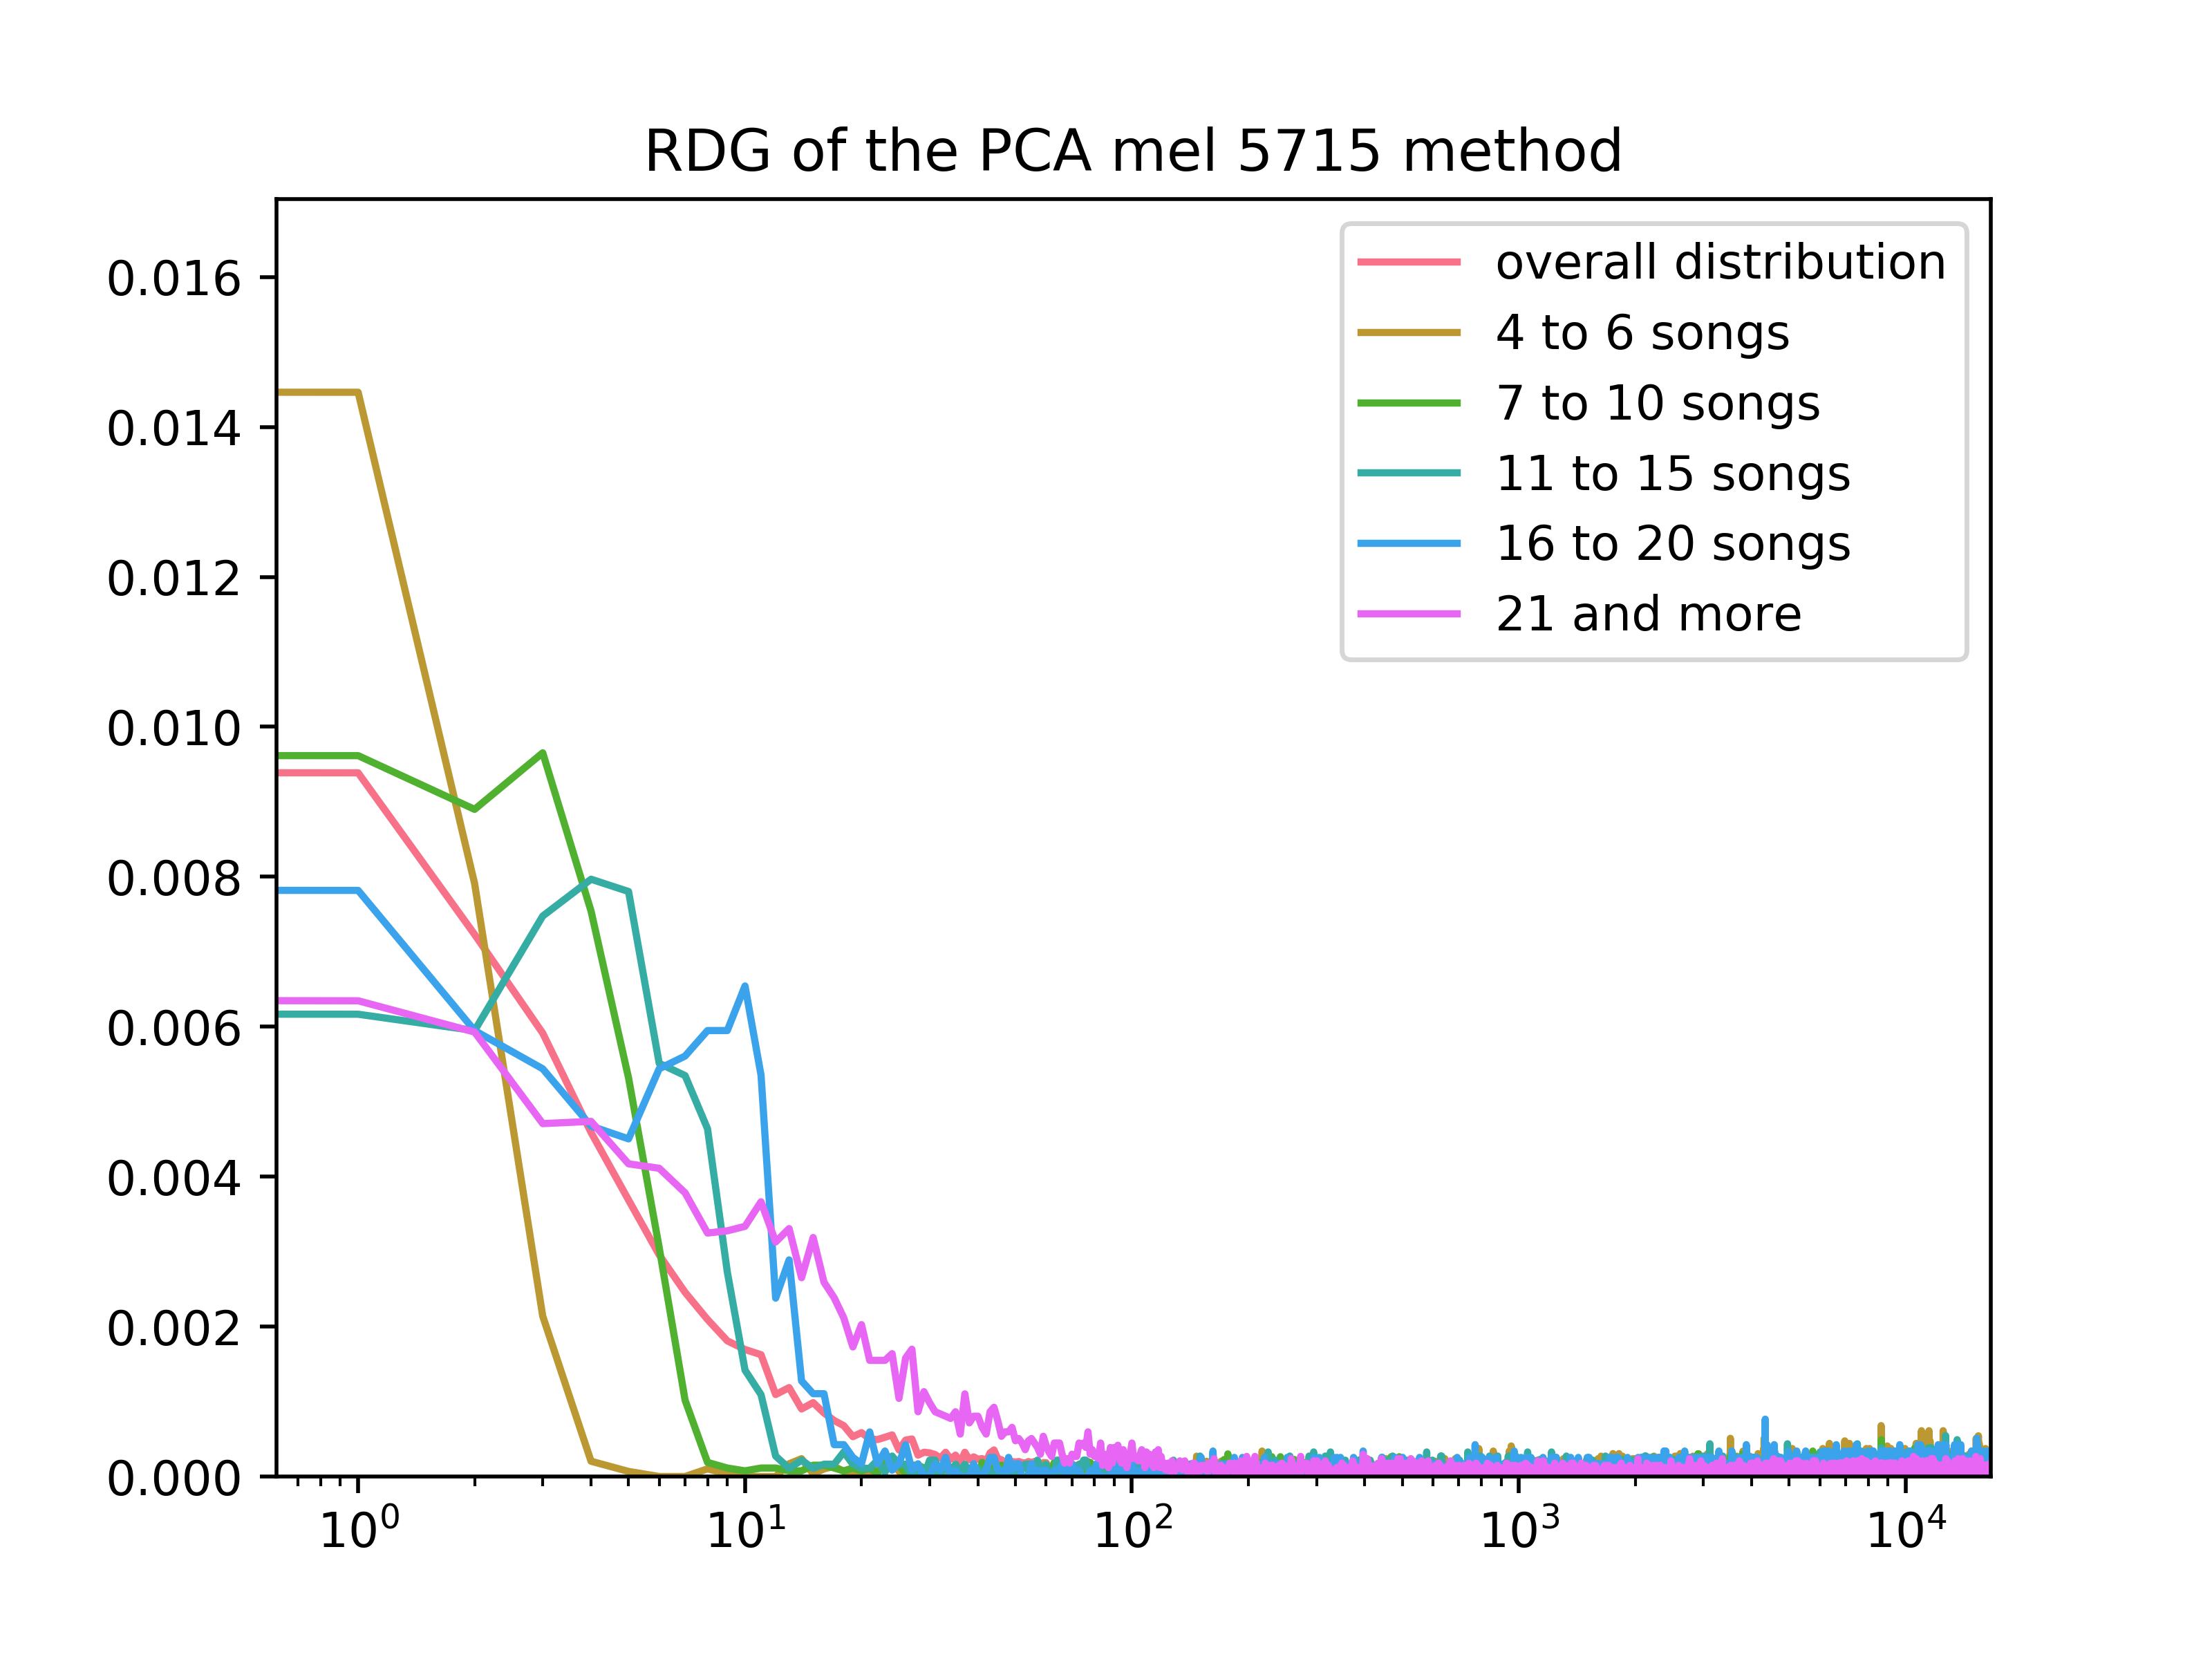
\includegraphics[width=1\linewidth]{./img/pca_mel_5715_graph.png}
  \captionof{Distribution of ranks of songs from the $p_{test}$ set the spectrogram method assigned them.}
  \label{fig:pca_mel_5715_distribution}
\end{minipage}%
\begin{minipage}{.5\textwidth}
  \centering
  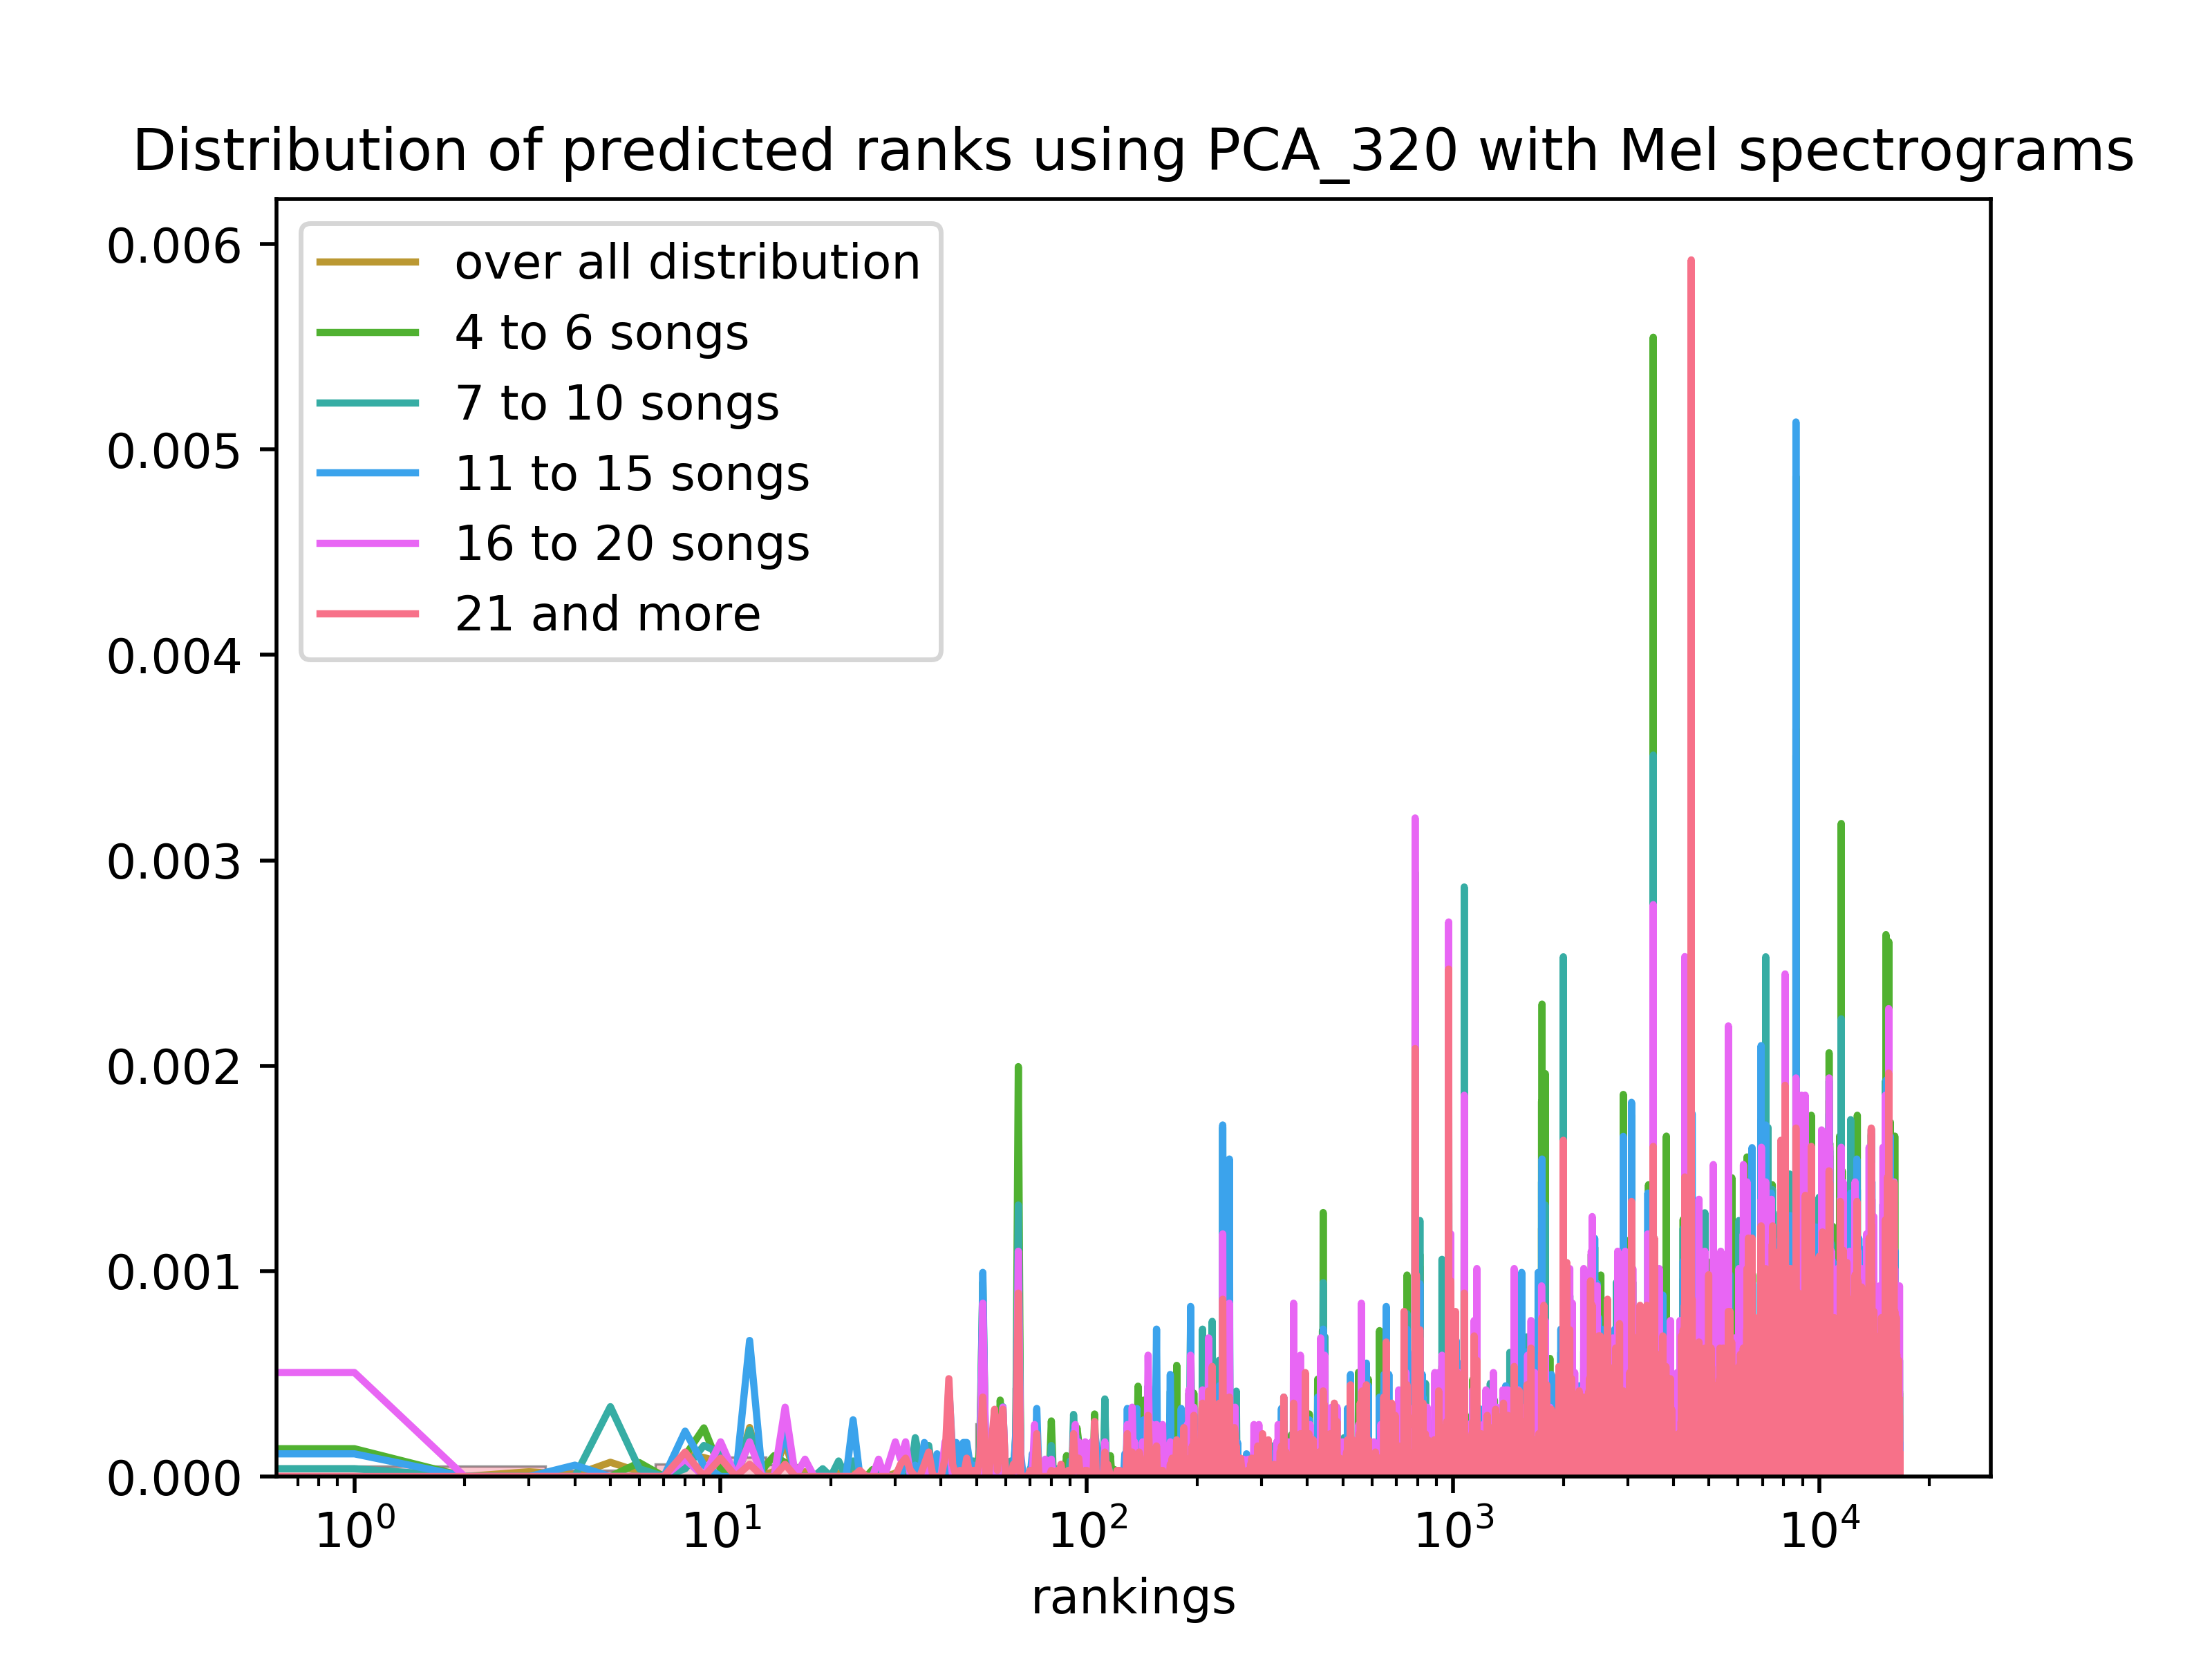
\includegraphics[width=1\linewidth]{./img/pca_mel_320_graph.png}
  \captionof{Distribution of ranks of songs from the $p_{test}$ for spectrogram vectors as input into PCA}
  \label{fig:pca_mel_320_distribution}
\end{minipage}
\end{figure}\label{fig:pca_mel_comparison_graps}

\section{Deep audio experiments}

\subsubsection{Architecture}
Before analysing each or the audio method using deep neural networks independently we will describe the two architectures we used. \\

As stated multiple times before, we decided to build our network based on the \cite{inproceedings_RNNs} paper. We chose our audio extraction coefficient based on their findings and we also designed our architecture in a way they did with some slight adjustments and extensions. \\

The first most notable thing is, that their network was designed to classify sounds, not encode songs. One might think that this would make their RNN unsuitable for our task, and it did as a whole. However their network consisted of two parts. The first part was an autoencoder and the second part a multi-layer perceptron. The autoencoder was trained in an unsupervised manner and the outputs were then fed into the MLP which did the classification. \\

For the purposes of our work, we only used the autoencoder part. Unlike them, instead of using the \texttt{auDeep} library we decided to build our networks with the \texttt{Keras} library \cite{chollet2015keras} as it has a user-friendly model creation API. We had also access to GPU computers and \texttt{Keras} (in our case with the \texttt{Tensorflow} backend) makes it easy to train networks faster with the access to GPUs. \\

We created two architectures. One with two GRU layers at the beginning as the encoder and one Bidirectional layer as the decoder. This follows the paper. We also decided to create another architecture with LSTM layers instead of GRU layers even though \citeauthor{inproceedings_RNNs} found in their work that the additional complexity did not yield better results. Both architectures can be seen in Figure \ref{fig:nn_architectures} \\

\begin{figure}[h!]
\centering
\begin{minipage}{.5\textwidth}
  \centering
  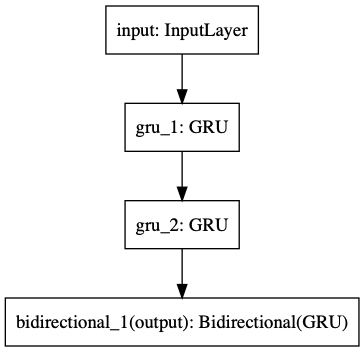
\includegraphics[width=1\linewidth]{./img/gru_architecture.png}
  \captionof{The general architecture of our GRU neural networks}
  \label{fig:gru_architecture}
\end{minipage}%
\begin{minipage}{.5\textwidth}
  \centering
  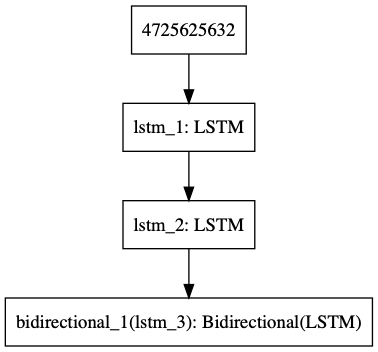
\includegraphics[width=1\linewidth]{./img/lstm_architecture.png}
  \captionof{The general architecture of our LSTM neural networks}
  \label{fig:lstm_architecture}
\end{minipage}
\end{figure}\label{fig:nn_architectures}


The main motivation behind using LSTMs as well as GRU layers in our thesis was that LSTM layers are specifically suited for sequential data such as audio. GRU layers are a simplified version of LSTMs. We were hoping that the more complex layers could encode our audio data into the same dimensions as the GRU networks but help to make the similarities more accurate. \\

We used the \textit{mean squared error} as our loss function which is the standard for autoencoder networks. Our optimiser was \textit{adam} the same as in the \cite{inproceedings_RNNs} paper. We had to decrease the learning rate from 0.001 to 0.0001. Before we did that, our resulting predicted vectors often consisted of just \textit{NaN}s.

\subsubsection{Inputs and outputs}
Both the GRU and the LSTM network had three kinds of inputs --- the spectrograms, mel-spectrograms and the MFCCs. They were all passed in the form of 2D matrices containing $(n\_features, n\_timestamps)$. GRU as well as LSTM networks take 2D matrices and not just 1D vectors as input. Before training, the inputs were normalized using the \texttt{MinMaxScaler} with values between 0 and 1. \\
One important thing to note here is that these kind of networks that process sequential data in the form of 2D matrices reduce the dimensionality of only the $n\_features$ and not the $n_{timestamps}$. Our 15 second audios yielded 408 time stamps and 2206 features for spectrograms and 408 time stamps and 320 features for mel-spectrograms. With MFCCs the number of time stamps was 646 and the number of features 128. Therefore we did not attempt a dimensionality reduction as big as with PCA which does not care if a feature is a time stamp or a sample.

\subsection{GRU network with spectrogram input}

\subsubsection{Training}

We trained two GRU spectrogram networks with variable output vector lengths. We decided to base our vector length on the PCA explained variance ratio. For spectrograms however, we only found out that 1106 explains 56\%of variance. Therefore, we took the information from the mel-spectrogram PCA where 5715 explains 90\% of variance and did a simple calculation $$ l(mel\_spec_{transformed})/l(mel\_spec) = l(spec_{transformed})/l(spec) $$. To keep the proportional reduction same as for mel-spectrograms and the output length of 5715 where $l(x)$ is the length of either the spectrogram or mel-spectrogram flattened. This would mean an output vector length of almost 40000. We decided that it would be too much for any practical use in our web application and reduced it to 20400 which at that point we thought could be potentially used. The shorter vectors used as encodings of our spectrograms were of length 5712. This inspired by the Mel-spectrogram PCA as we thought that the neural network could mimic the Mel-frequency reduction as well as additional reduction. \\
In our base paper, they trained their autoencoders for 50 epochs using batch sizes of 64. We found this to be insufficient especially with our learning rate reduction. For GRU networks with spectrograms we set the number of epochs to 100 and the batch size to 295 (for higher batch values we got memory errors). 

\subsubsectiom{Results}
As can be observed in Figure \ref{fig:all_model_training} the loss is basically constant for both GRU networks with spectrogram input (the GRU\_spec\_20400 is hidden behind the orange line of GRU\_spec\_5712 as their progress or rather the lack of it is the same). This means, that the network did not really improve for some reason. Therefore it is not suprising that the results of this method are not between our best ones.

We can see in Table \ref{table:spec_methods} that only 0.2\% of songs was ranked in the top 10, 0.5\% in the top 50 and 1\% in the top 100 for the longer GRU spectrogram model. For the short GRU spectrogram model, the results are a slightly better with 0.2\% for the top ten songs 0.6\% ranked in the top 50 and a little over 1\% ranked in the top 100. The ranking improvement is just very small and almost non-existent when rounding the numbers to two decimal places and then converting them into percentages. \\
The distributions depicted in Figure \ref{fig:gru_spec_distributions} of both GRU\_specs is are similar too. The trend for worse ranks for songs from longer playlists is apparent in both method graphs but it is not as obvious as in methods that have over all better results.

\begin{figure}[h!]
\centering
\begin{minipage}{.5\textwidth}
  \centering
  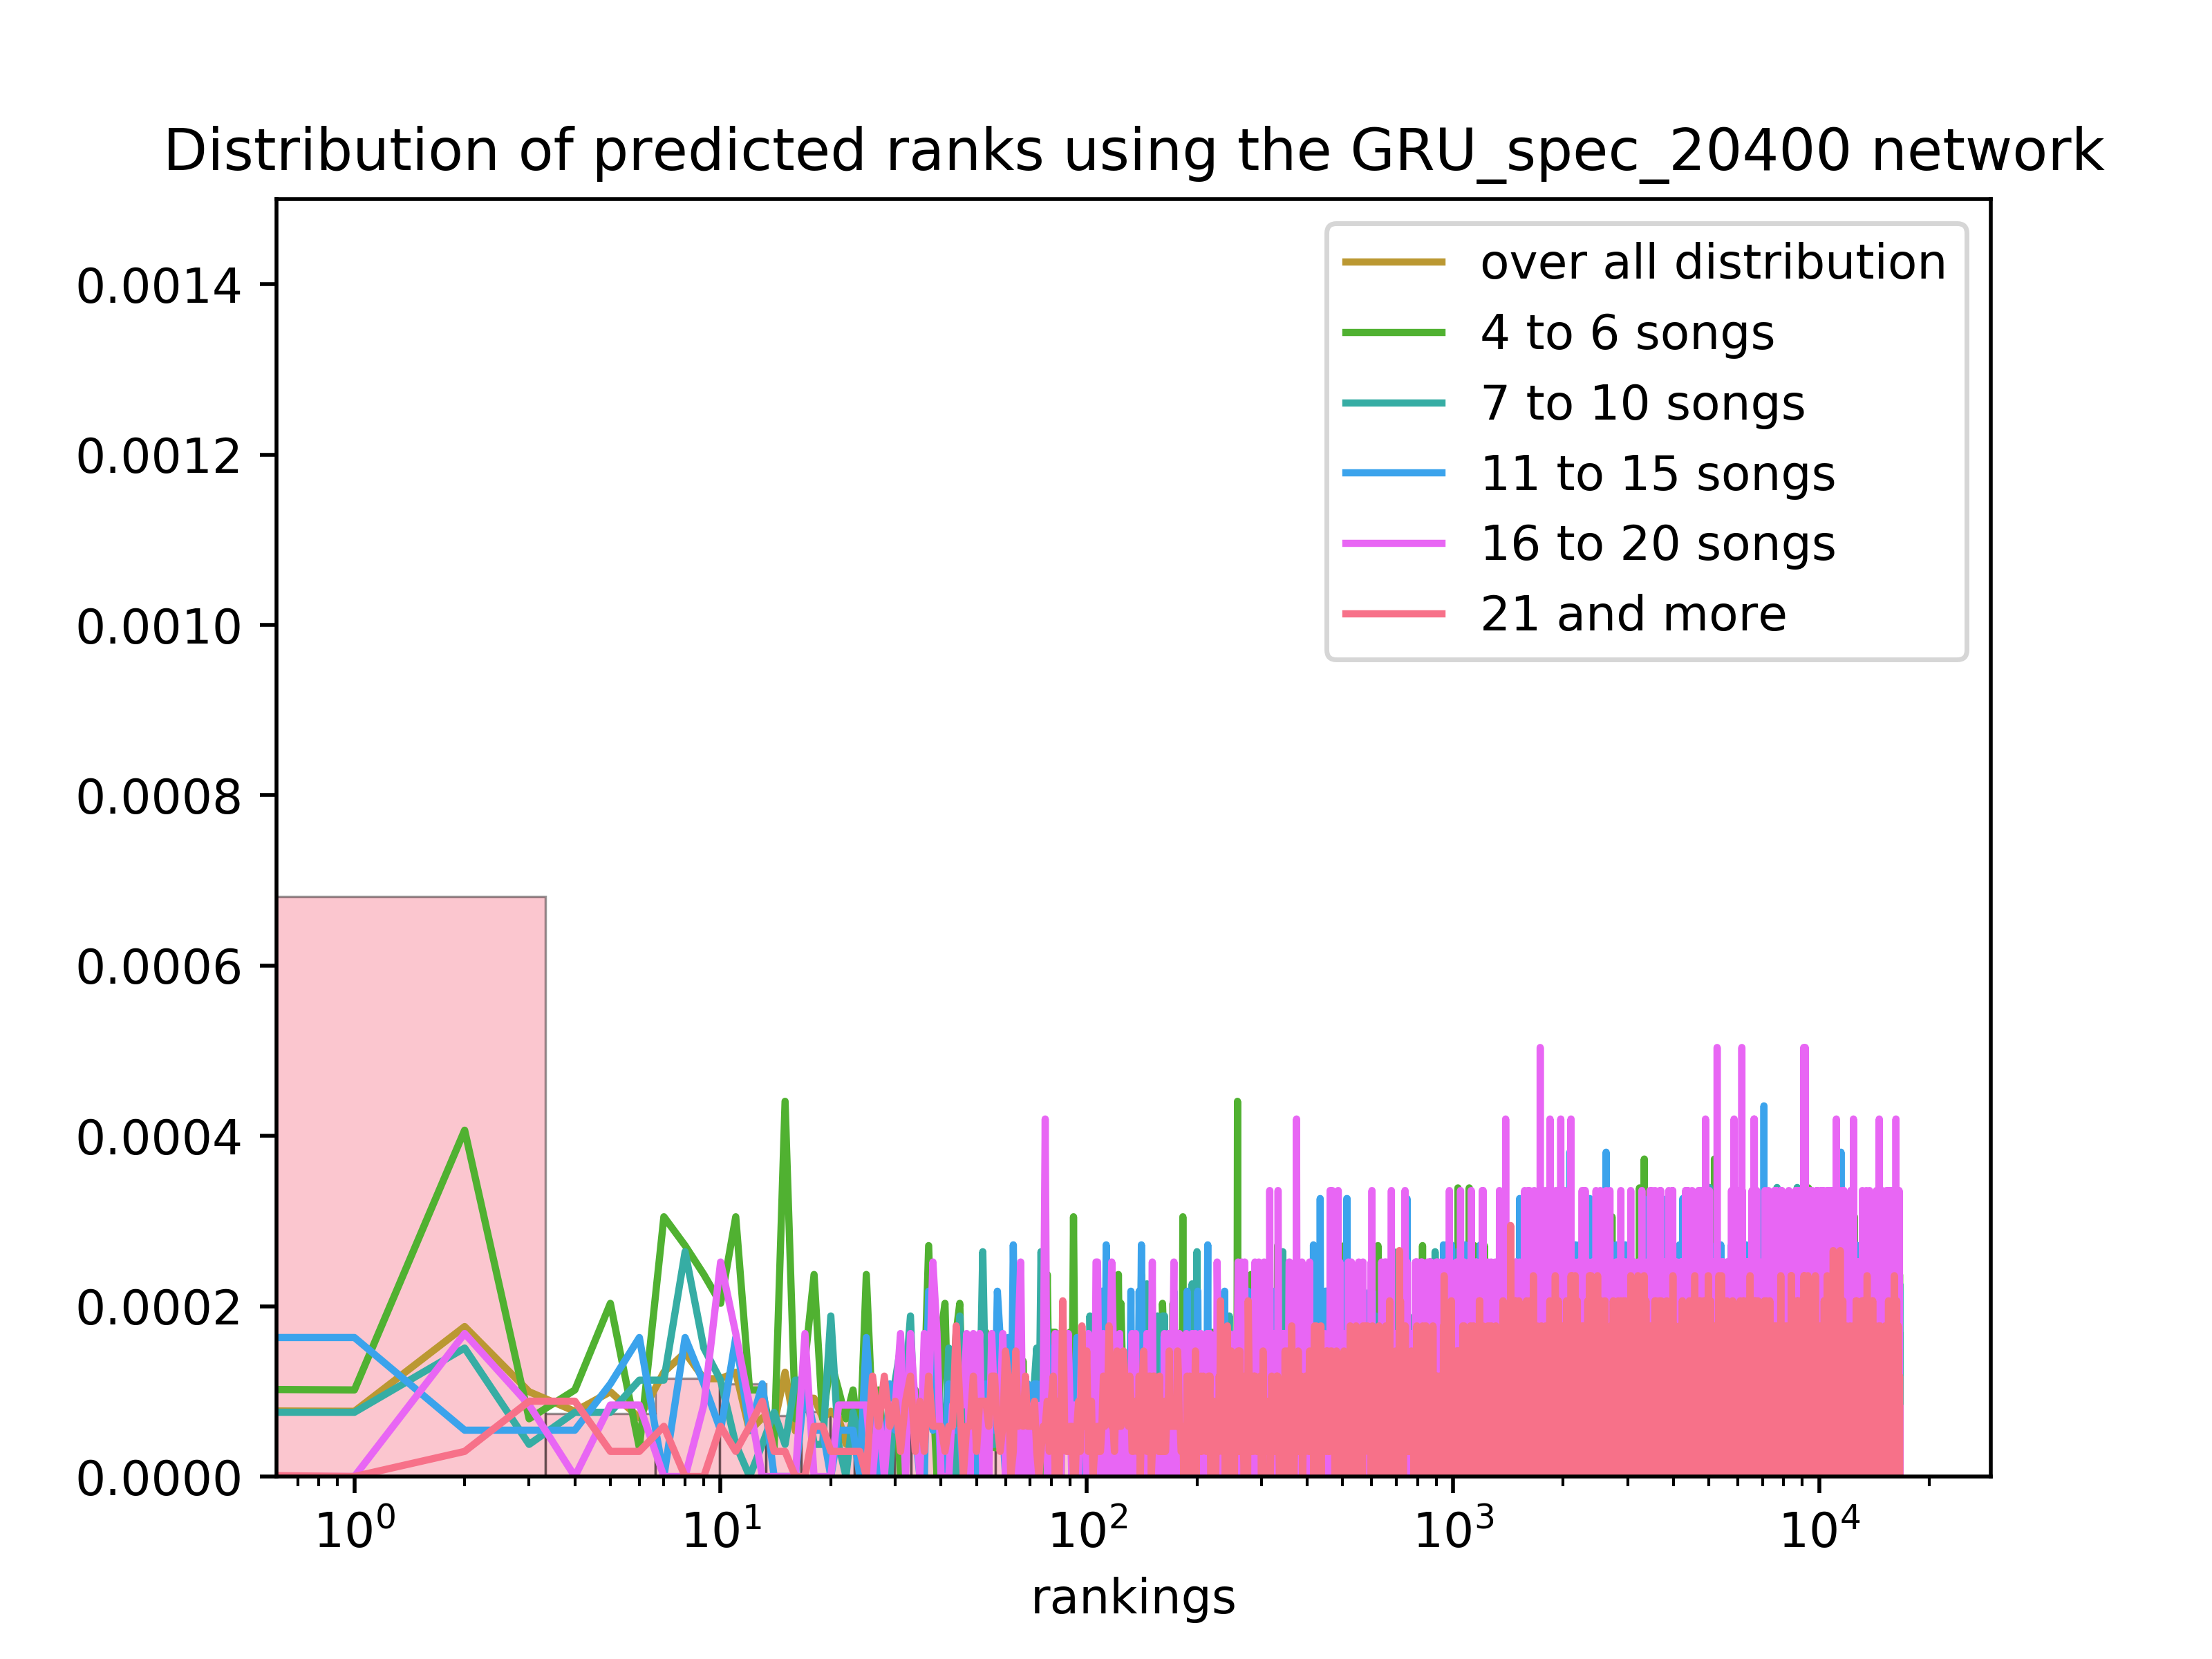
\includegraphics[width=1\linewidth]{./img/gru_spec_20400_graph.png}
  \captionof{The distribution of predicted ranks using the long GRU spec encodings.}
  \label{fig:gru_spec_20400_distribution}
\end{minipage}%
\begin{minipage}{.5\textwidth}
  \centering
  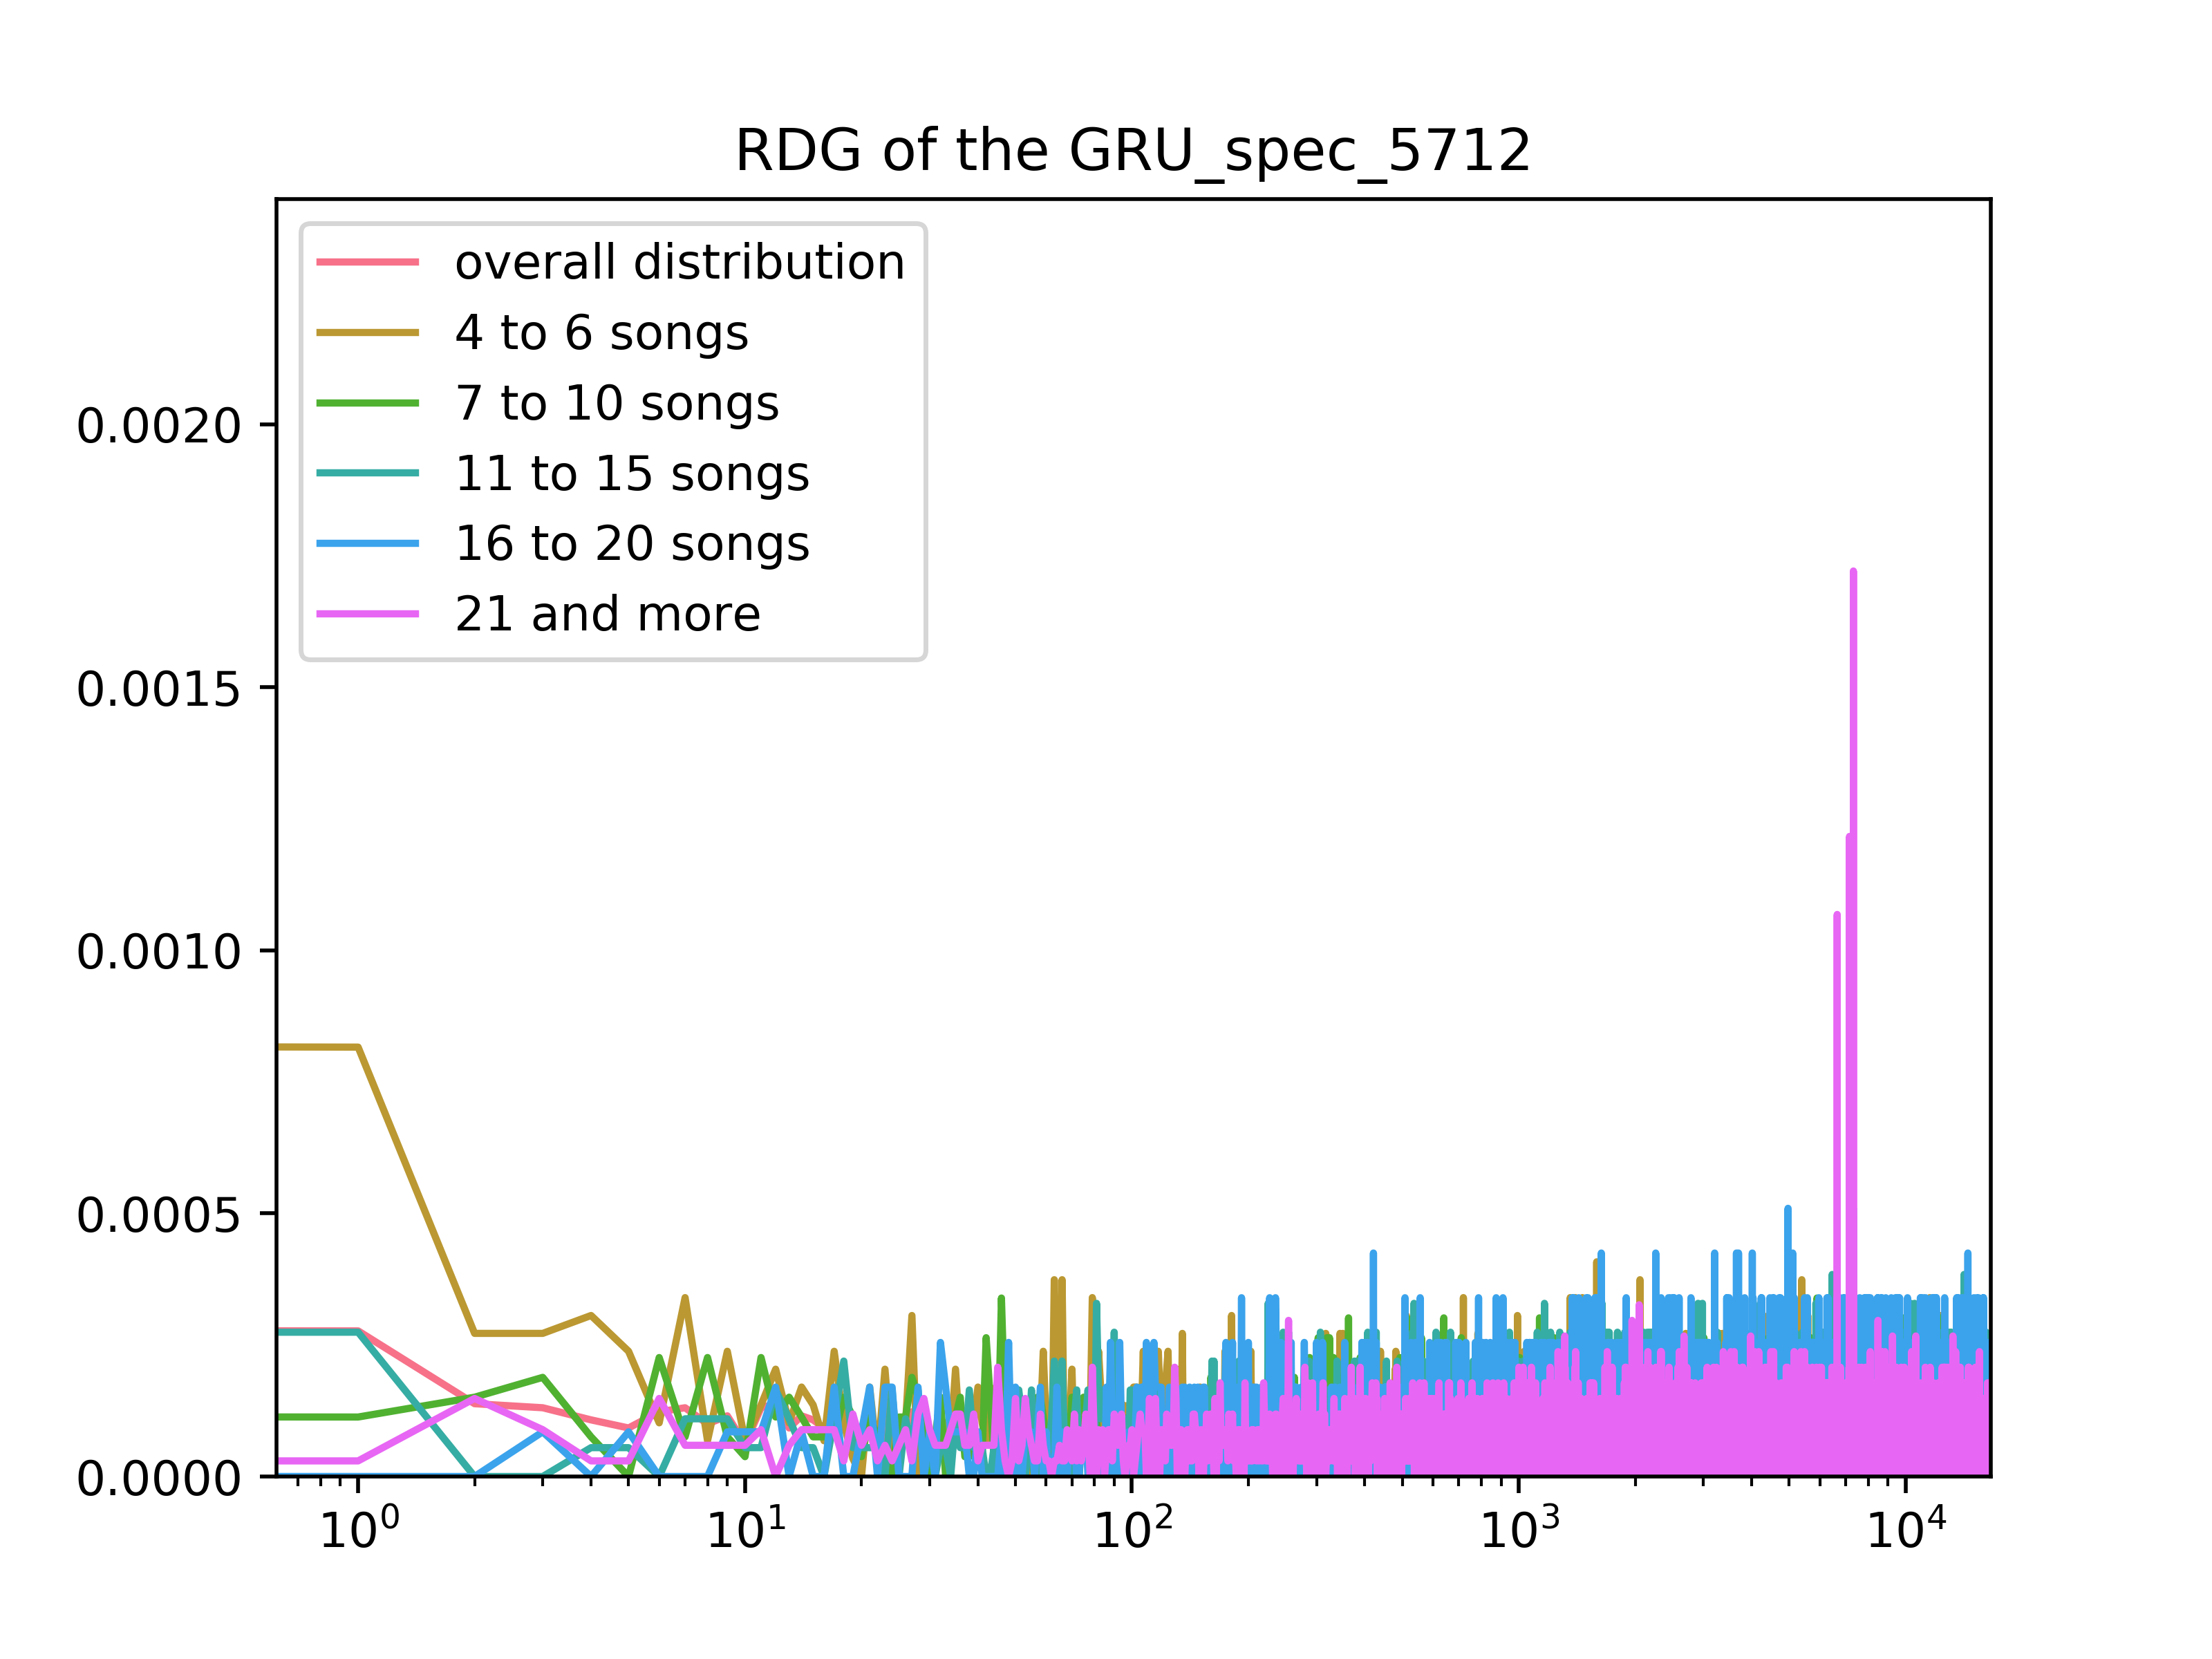
\includegraphics[width=1\linewidth]{./img/gru_spec_5712_graph.png}
  \captionof{The distribution of predicted ranks using the short GRU spec encodings.}
  \label{fig:gru_spec_5712_distribution}
\end{minipage}
\end{figure}\label{fig:gru_spec_distributions}

\subsection{LSTM network with spectrogram input}

\subsubsection{Training}
We chose the same training strategy for LSTMs with spectrogram input as we did for the GRU\_spec networks. It makes the comparison of both methods more fair under the same conditions. We also created two versions of our LSTM models, one LSMT\_spec\_20400 and the shorter version LSTM\_spec\_5712. The lengths are the same as with GRU\_specs and the motivation behind them is identical.

\subsubsection{Results}
Unlike the GRU model training which showed almost no improvement even after 100 epochs of training, our LSTM\_specs as one can observe in Figure \ref{fig:all_model_training} where the LSTM\_spec\_20400 is rendered in green and the LSTM\_spec\_5712 in red went through at least some progress. The decrease of loss slowed down significantly towards the end of the 100 epochs. \\
The higher training improvement correlates with better results for the LSTM\_spec methods. In Table \ref{table:spec_methods} are both the results of the LSTM\_spec models. They are better than those of the GRU\_spec models. \\
A thing worth noting here is that with the shorter encoding vector the results worsened. Definitely more dramatically than how the GRU\_spec results imporoved. The values in Table \ref{table:spec_methods} and distribution in Figure \ref{fig:lstm_spec_distributions} visualize the difference clearly, especially when it comes to songs from short playlists where the difference most apparent.

\begin{figure}[h!]
\centering
\begin{minipage}{.5\textwidth}
  \centering
  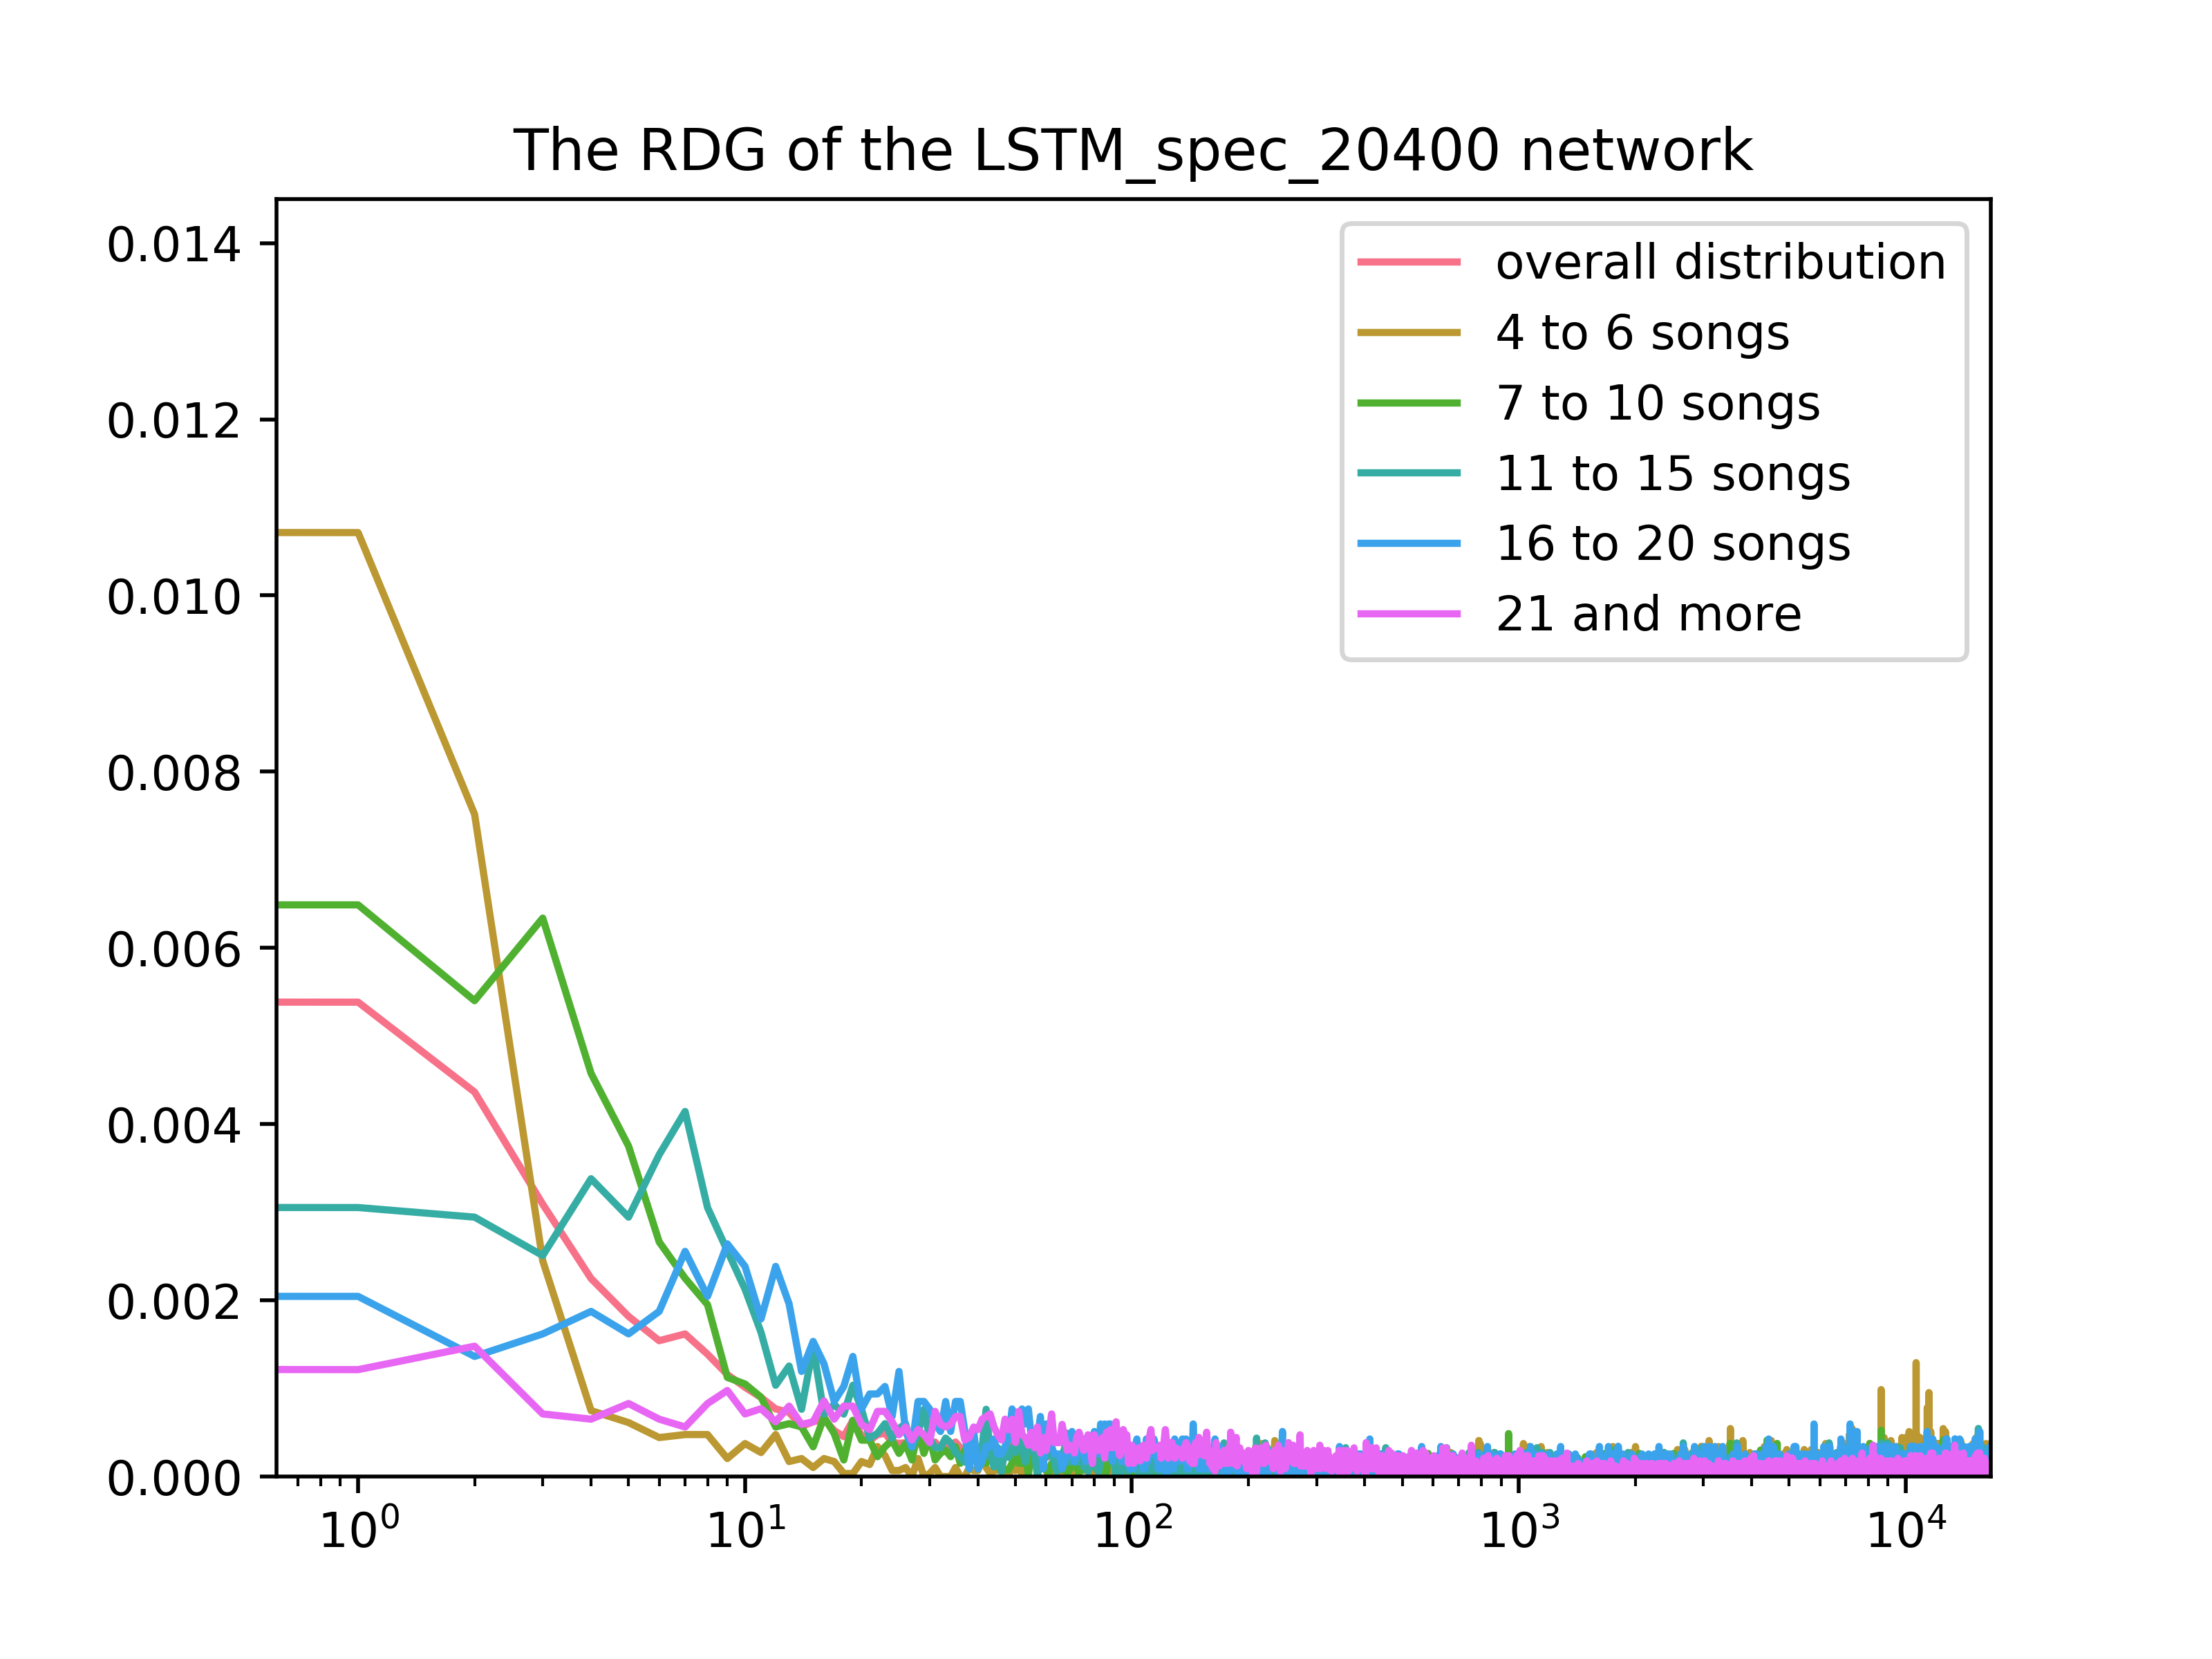
\includegraphics[width=1\linewidth]{./img/lstm_spec_20400_graph.png}
  \captionof{The distribution of predicted ranks using the long GRU spec encodings.}
  \label{fig:lstm_spec_20400_distribution}
\end{minipage}%
\begin{minipage}{.5\textwidth}
  \centering
  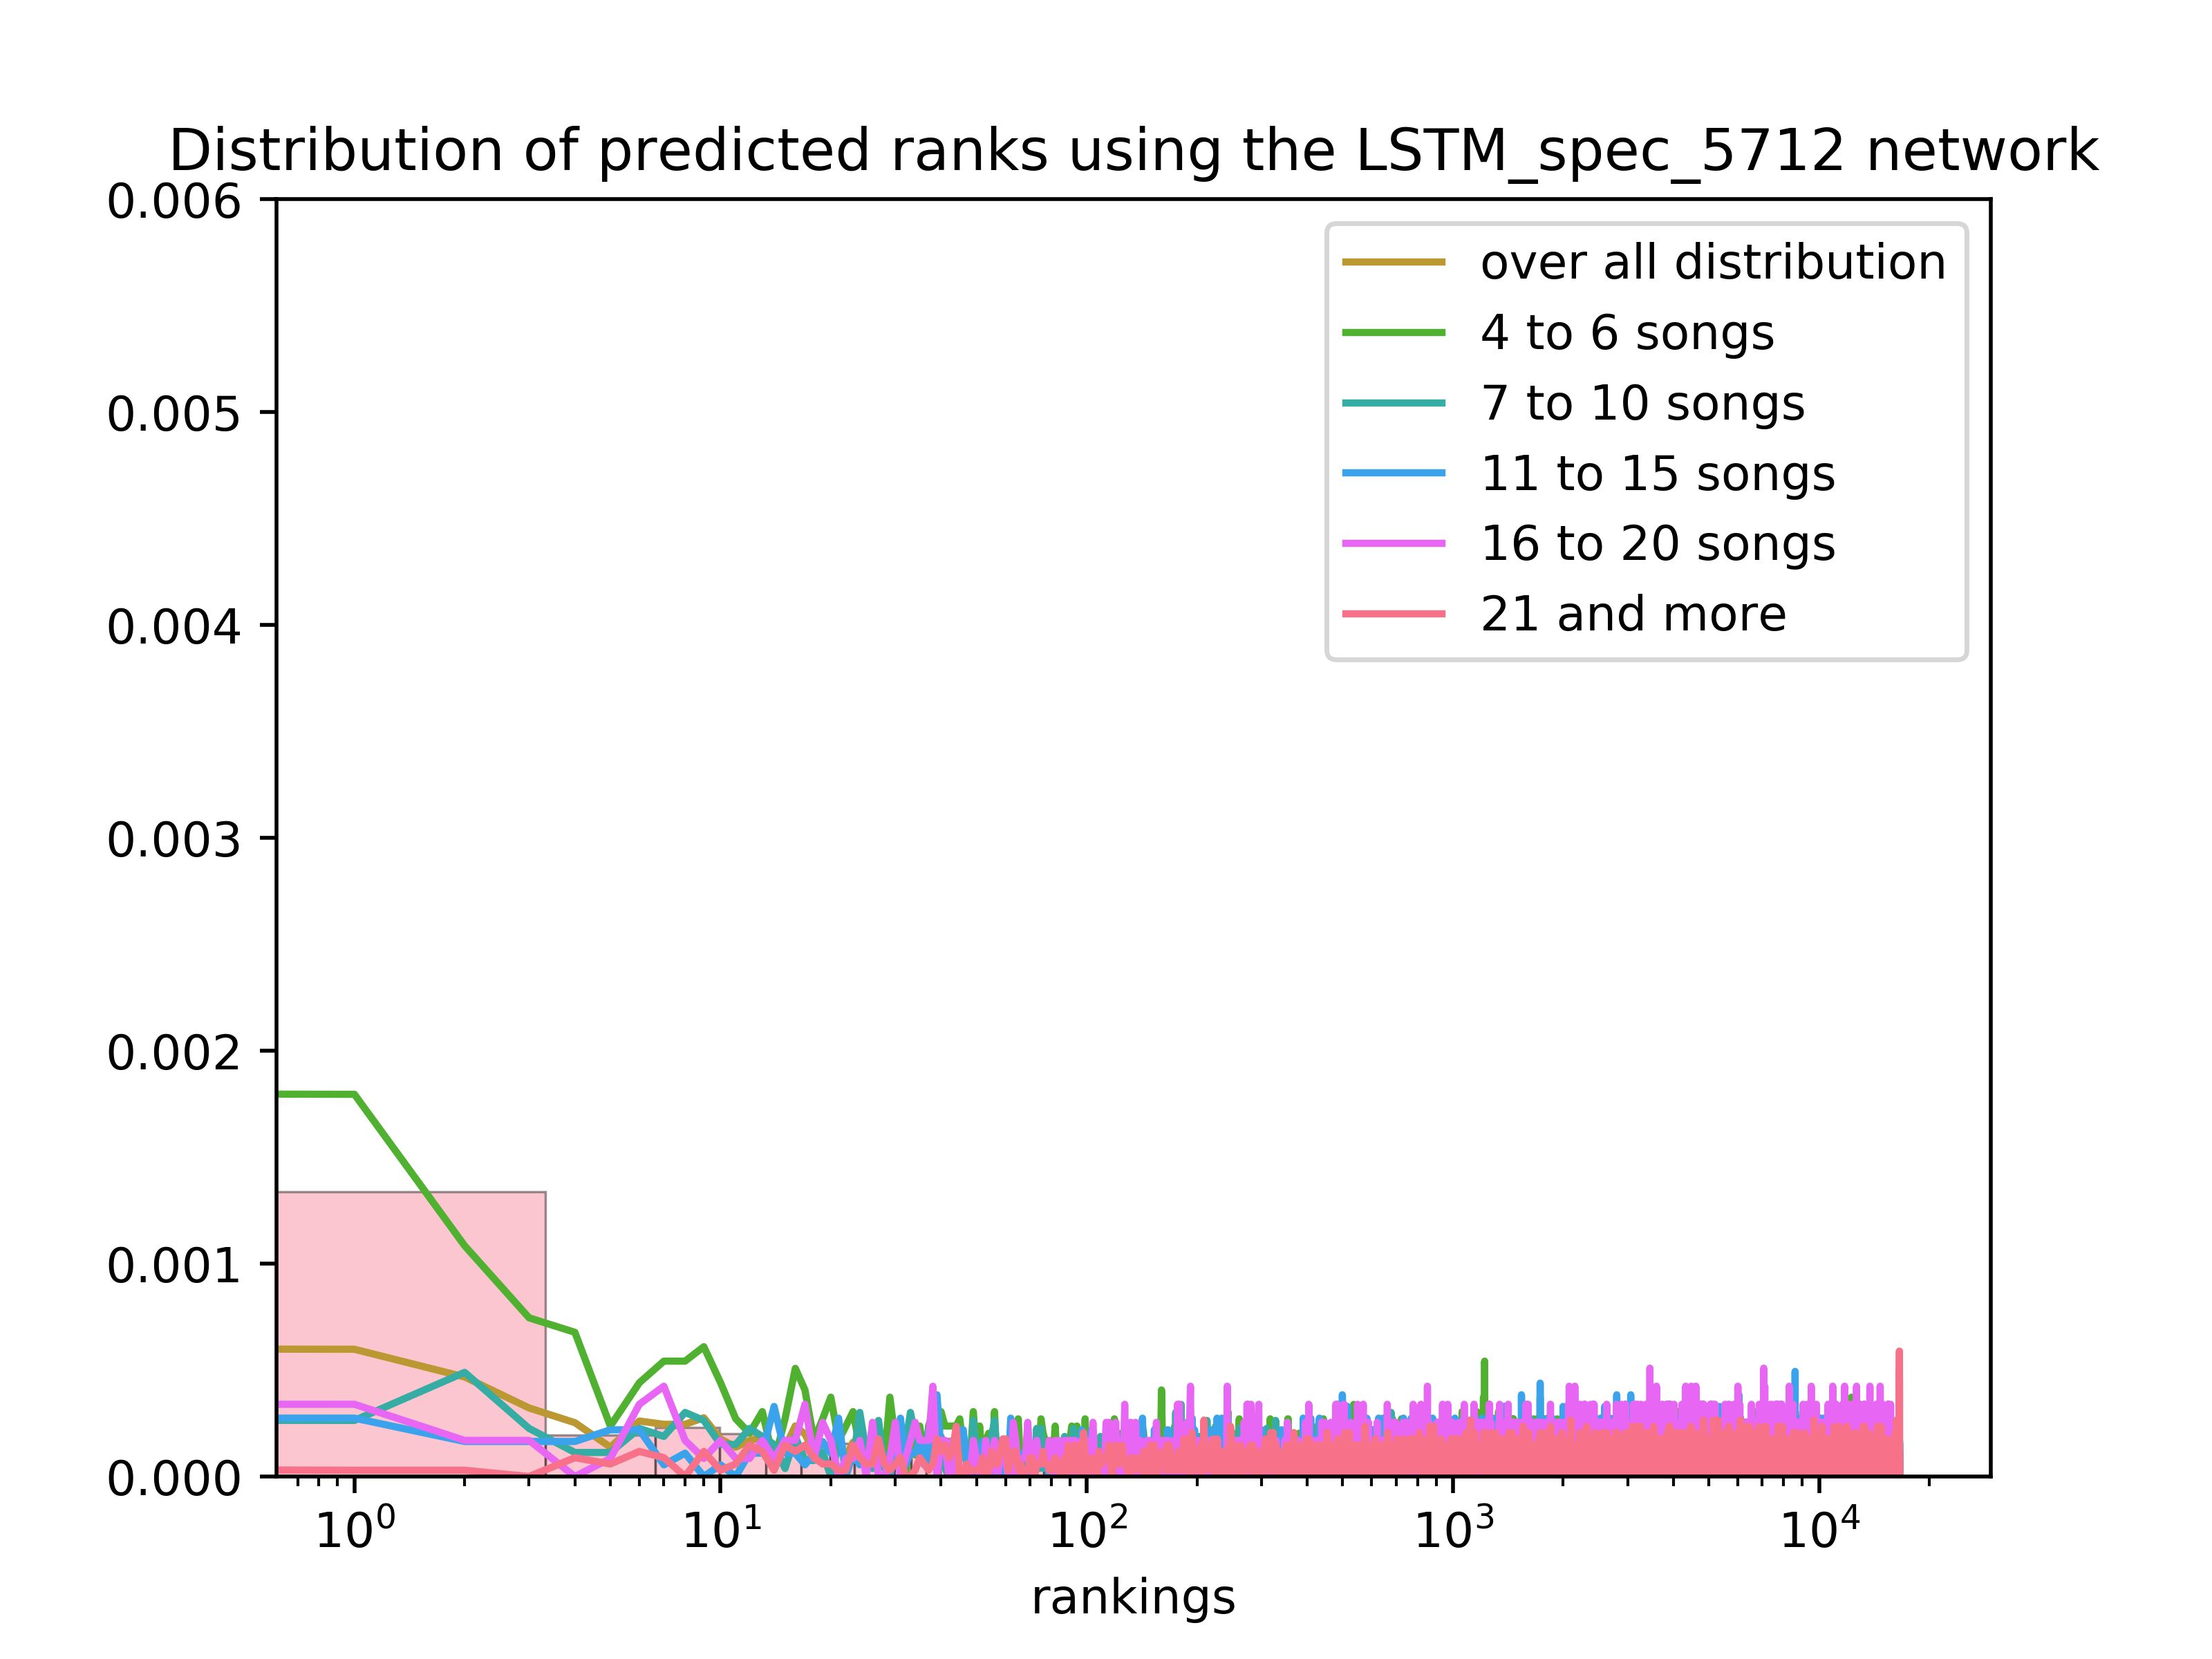
\includegraphics[width=1\linewidth]{./img/lstm_spec_5712_graph.png}
  \captionof{The distribution of predicted ranks using the short GRU spec encodings.}
  \label{fig:lstm_spec_5712_distribution}
\end{minipage}
\end{figure}\label{fig:lstm_spec_distributions}

\subsection{GRU and LSTM networks with Mel-spectrogram input}

\subsubsection{Training}
The GRU\_mel and LSTM\_mel networks were both trained under the same conditions. We trained them on our mel-spectrograms for 150 epochs with a batch size of 256. With a higher batch size we got a memory error. The output length of the encoded song vector was based on variance ratio of the PCA\_mel (same as for networks with neural networsk with spectrogram input). We did not attempt any further reductions here partly because further dimensionality reduction in PCA\_mel\_320 greatly hurt the performance and partly because as stated before, only the features can be reduced by GRU and LSTM layers meaning, that we have to have vectors of length of at least 408 and to scale the features down to one or two might lead to same results as with our SOM methods.

\subsubsection{Results}
Mel-spectrograms seem to be the best kind of input we have and the GRU\_mel and LSTM\_mel networks confirm it as they have the best results within the neural network method group. The GRU\_mel network performed better than the one with LSTM layers and also showed the smallest loss in training. The difference in ranking accuracy is quite big. Figure \ref{fig:mel_nn_distributions} exposes another thing worth noting which the big difference between short and long playlist rankings for both methods. \\
Table \ref{table:mel_spec_methods} puts recalls and nDGC of our "mel" neural networks into perspective with other "mel" methods.
As we can see, the GRU\_mel network placed 3.6\% of songs into the top 10, 4.3\% into the top 50 and 4.9\% into the top 100. This is worse than the raw mel-spectrogram method for \textit{R@10} but for \textit{R@50} and \textit{R@100} it shows better results. The GRU\_mel network is almost twice as bad and places as our second worst "mel" method with only 1.4\% of songs in the top 10, 2\% of songs in the top 100 and 2.6\% of songs with assigned ranks in the top 100.

\begin{figure}[h!]
\centering
\begin{minipage}{.5\textwidth}
  \centering
  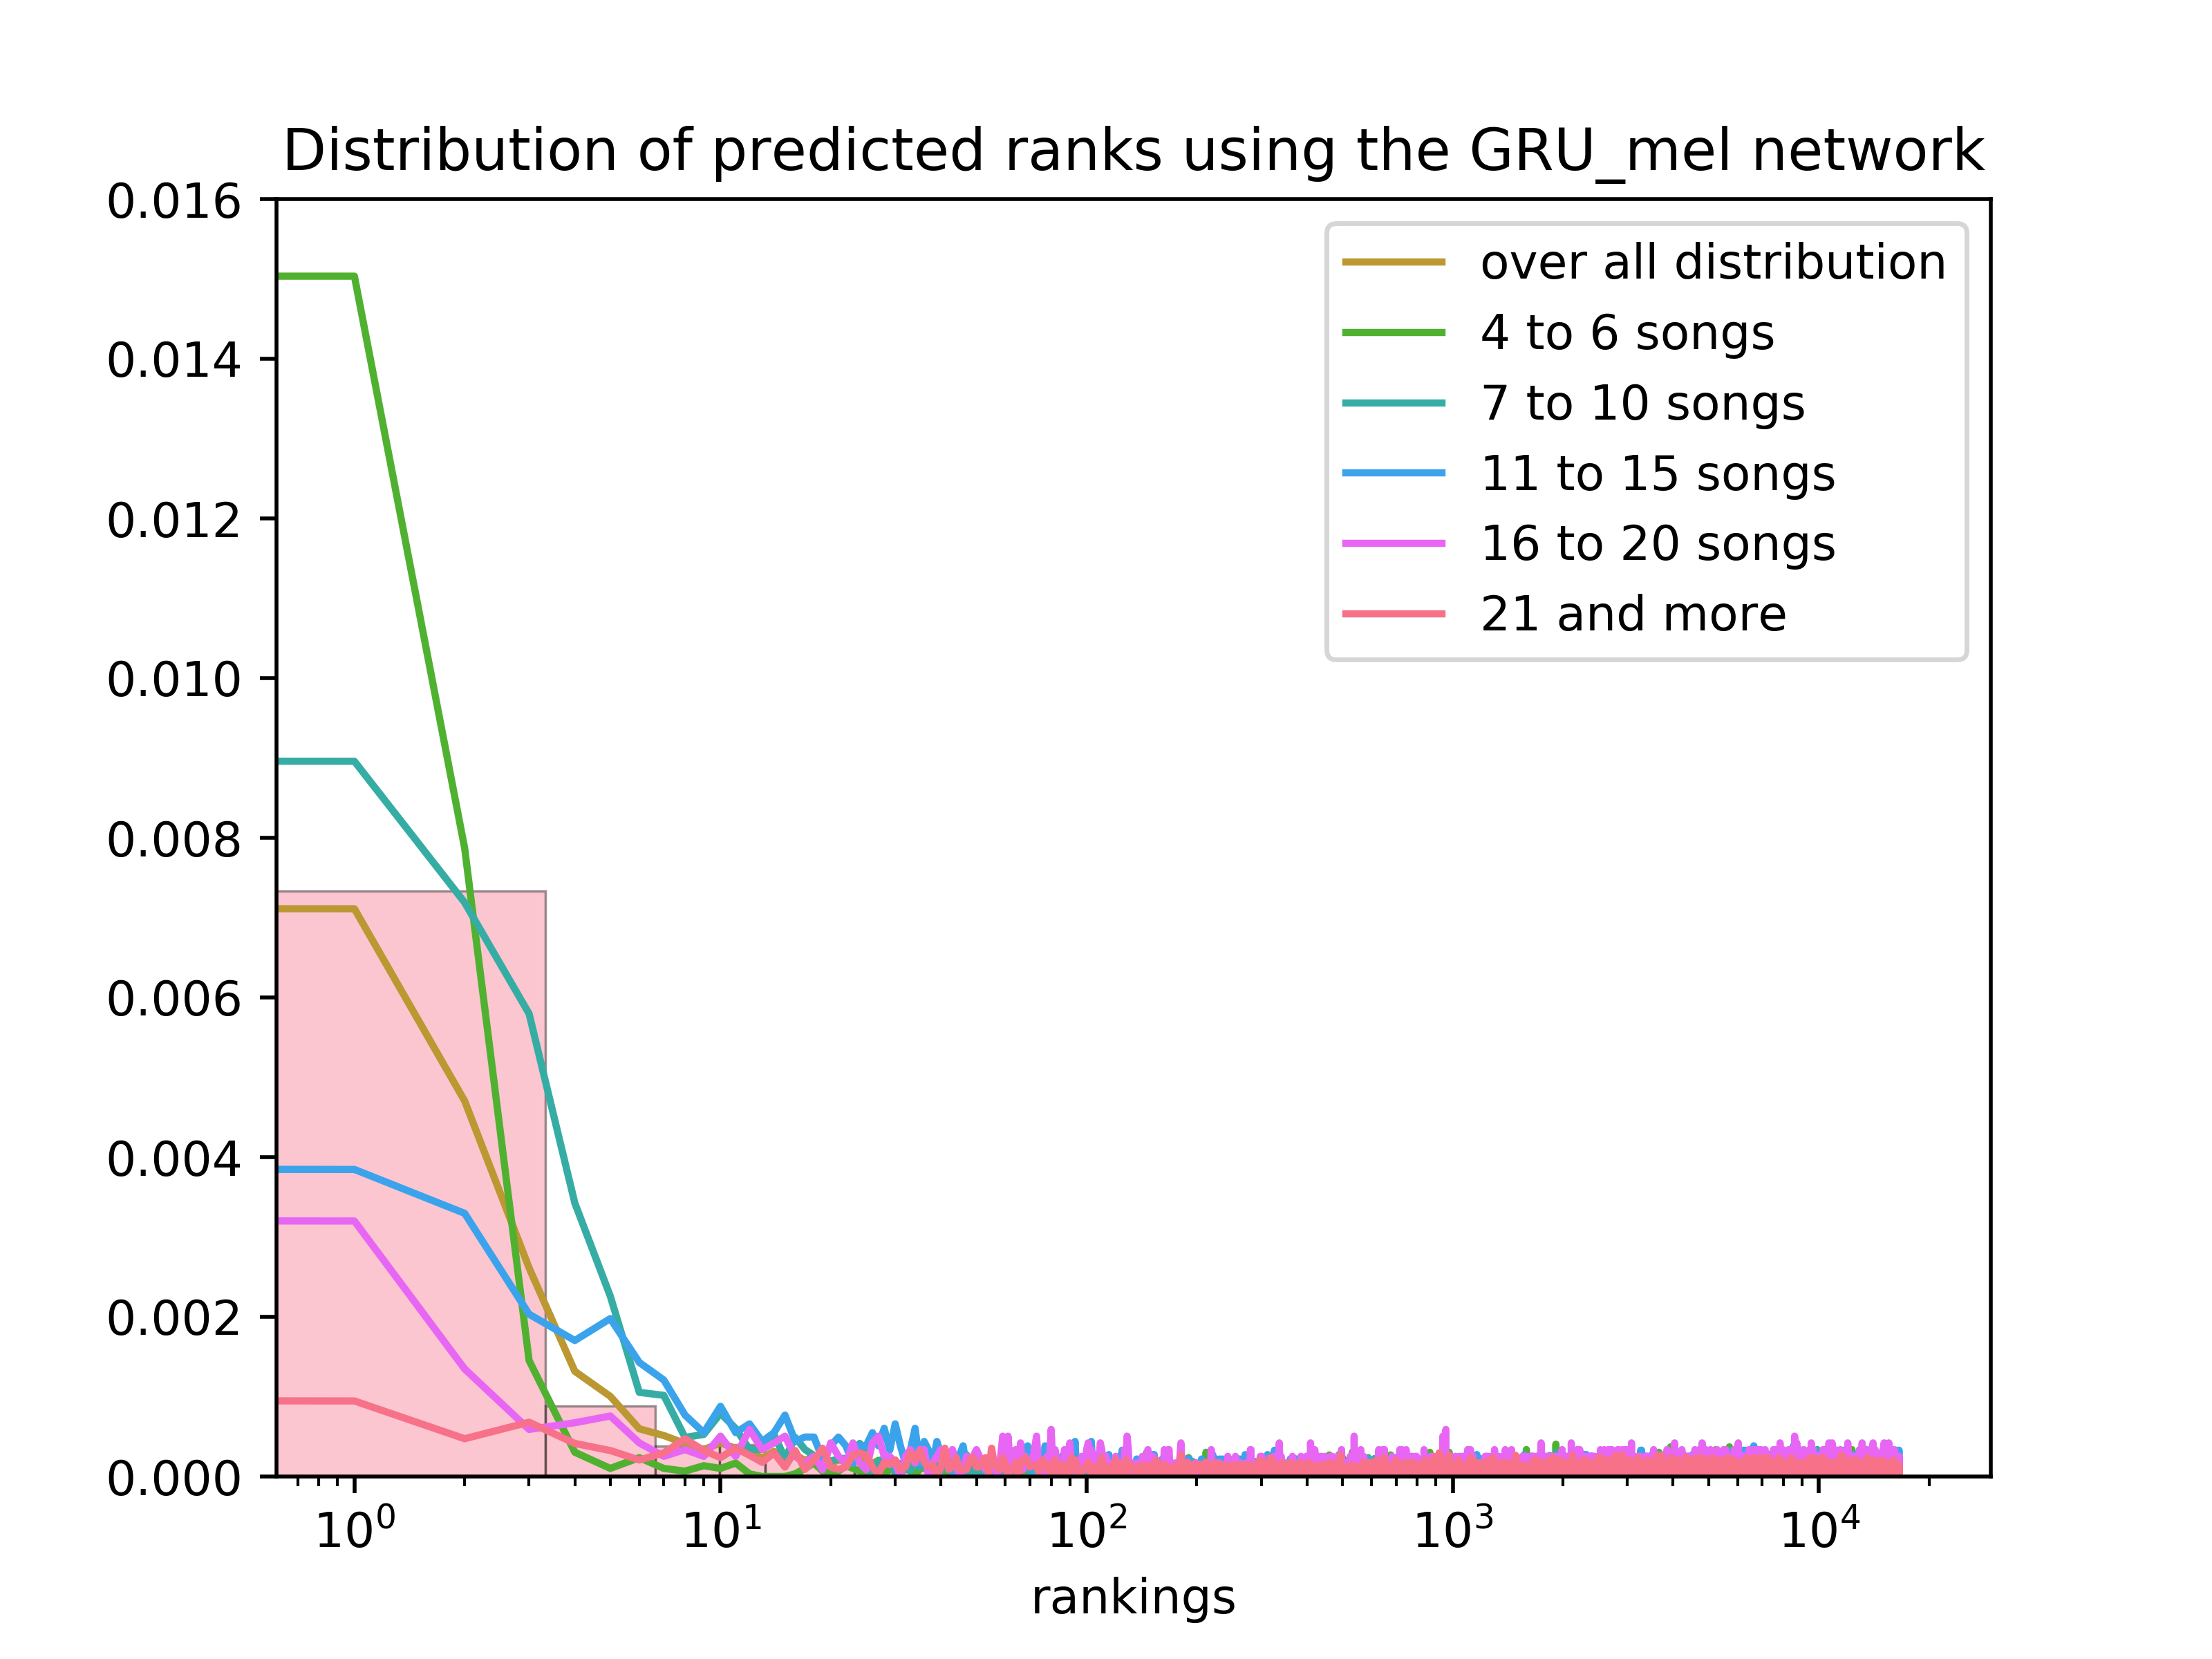
\includegraphics[width=1\linewidth]{./img/gru_mel_graph.png}
  \captionof{An RDG of the GRU\_mel method}
  \label{fig:gru_mel_distribution}
\end{minipage}%
\begin{minipage}{.5\textwidth}
  \centering
  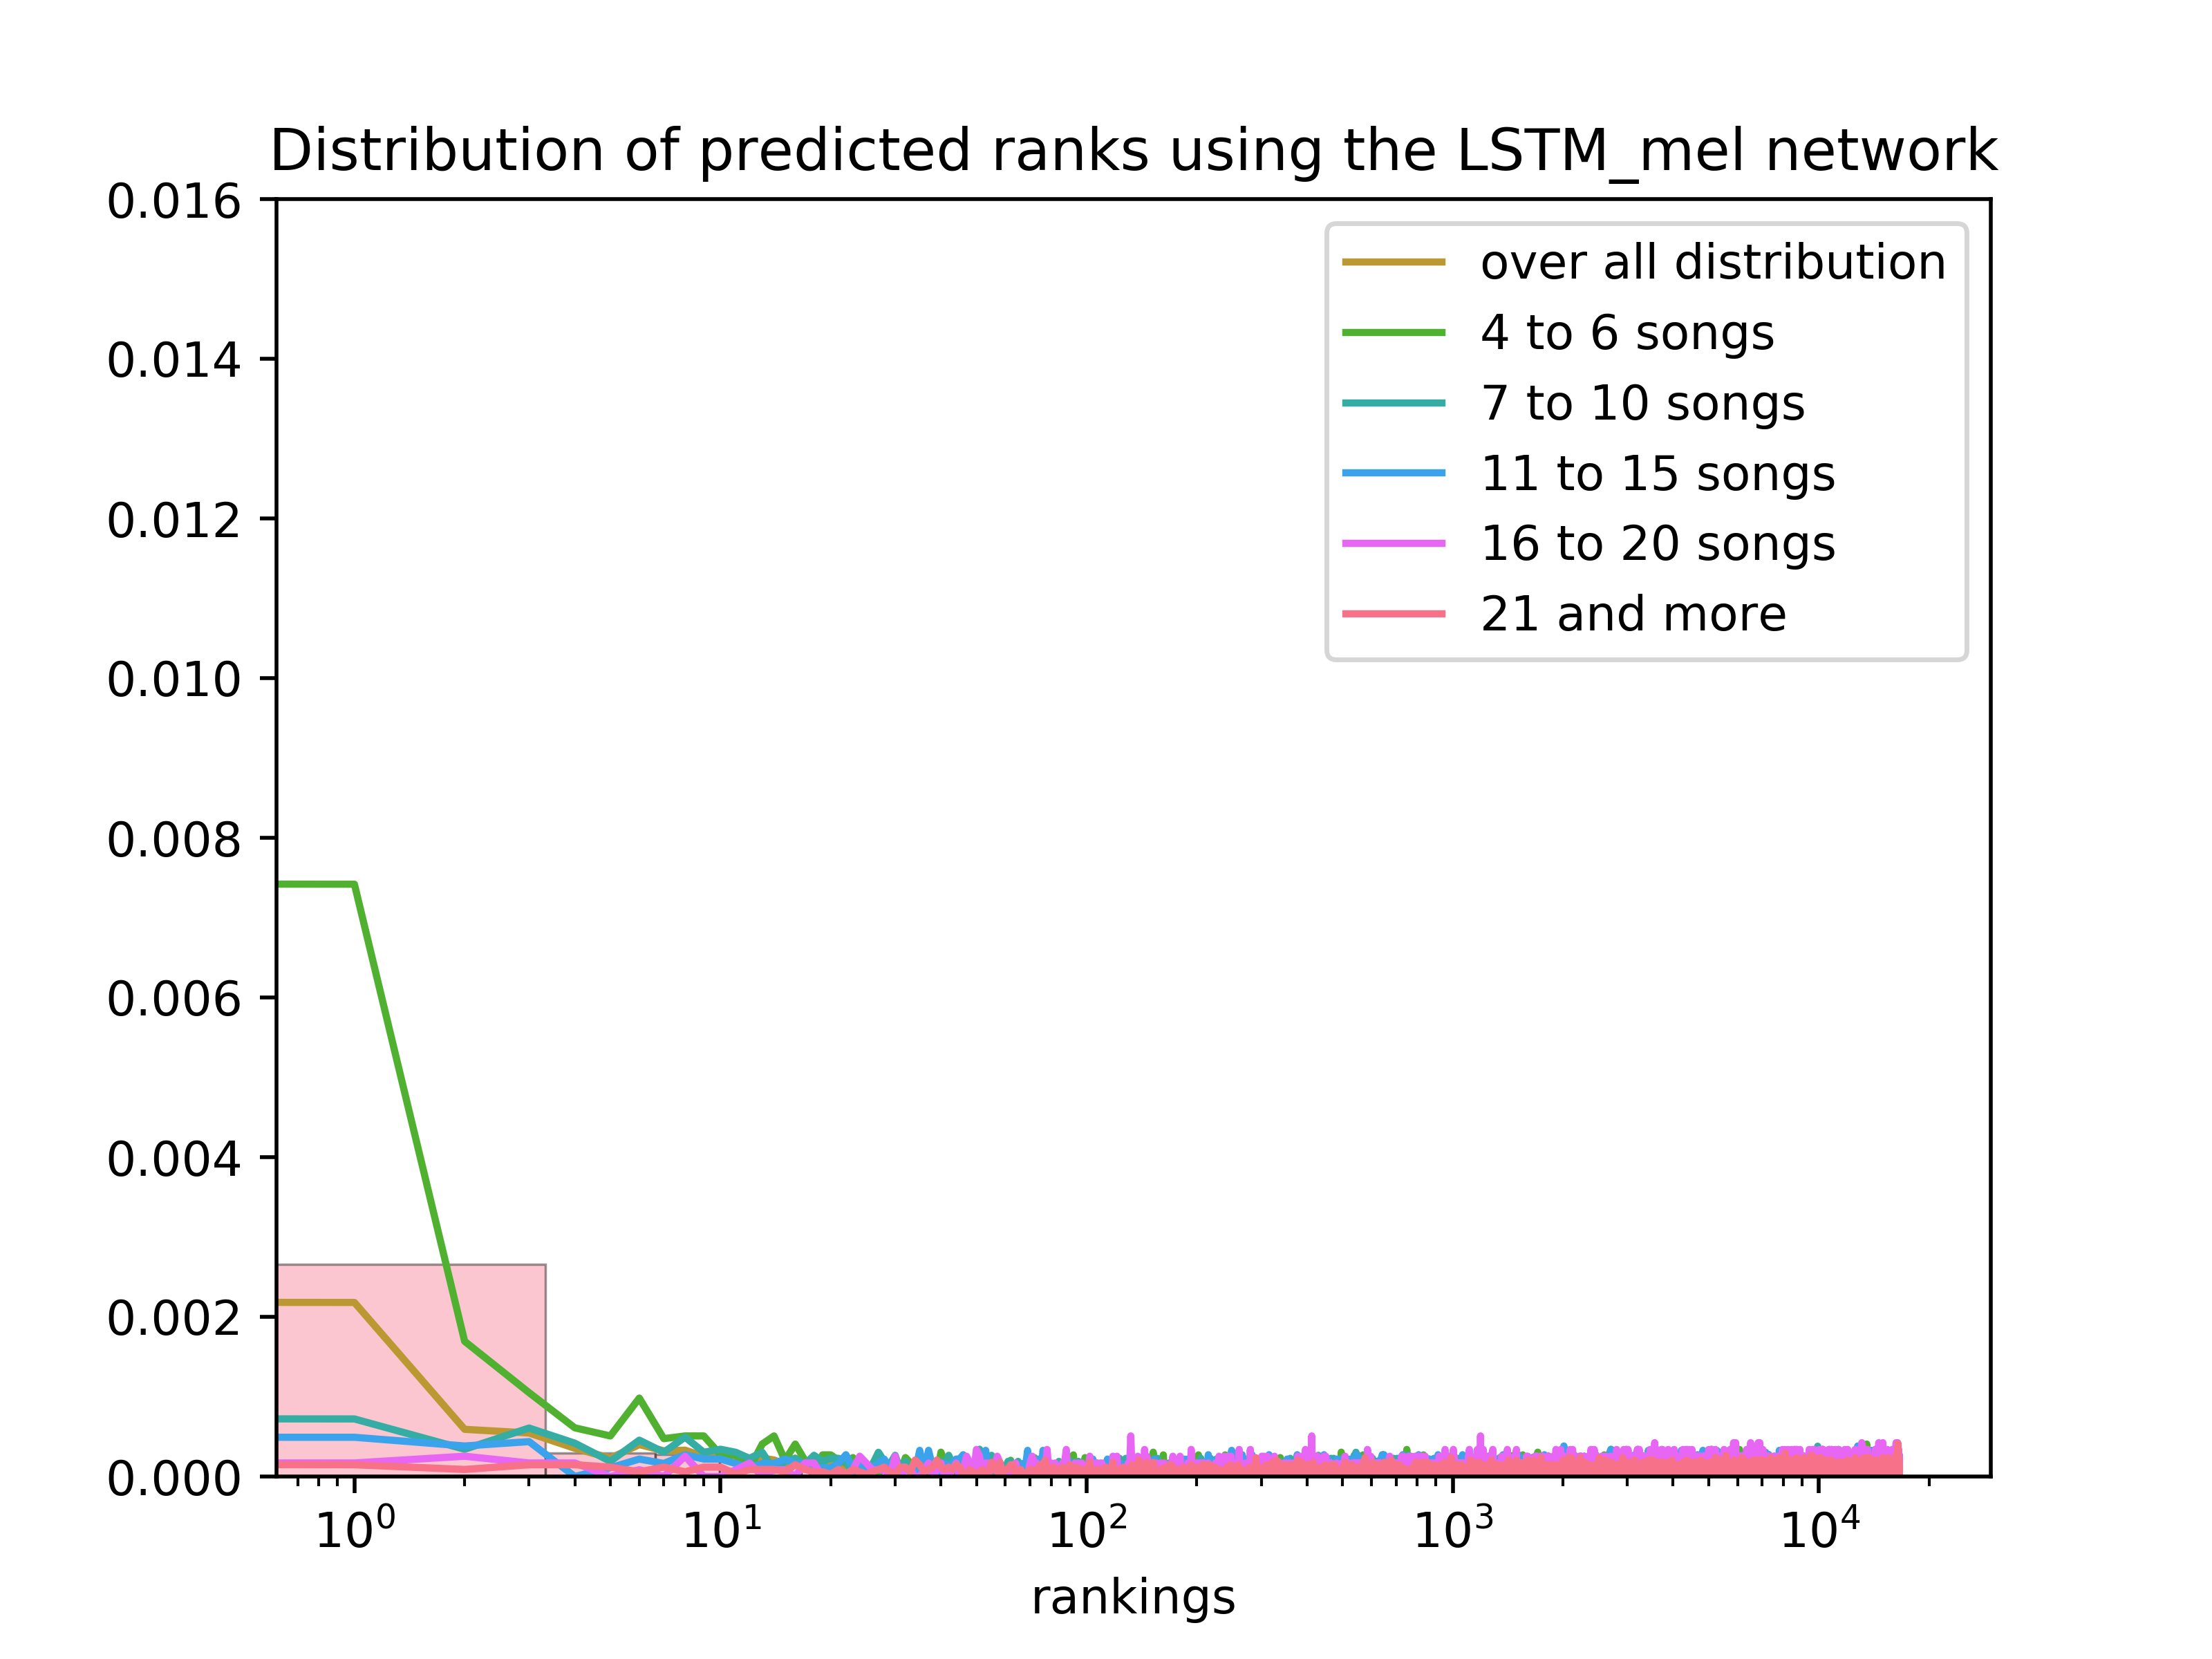
\includegraphics[width=1\linewidth]{./img/lstm_mel_graph.png}
  \captionof{An RDG of the LSTM\_mel method}
  \label{fig:gru_mel_distribution}
\end{minipage}
\end{figure}\label{fig:mel_nn_distributions}

\subsection{GRU and LSTM networks with MFCC input}

\subsubsection{Training}
At first we did not plan on using MFCCs as input into neural networks. However because it turned out the the raw MFCCs are too long to be used in our application directly we decided it would be a shame to just leave them out and tried to reduce their dimension again with both our GRU and LSTM network architectures. \\ 
We trained both architectures with 150 epochs and a batch size of 256 which is the same as the neural networks having mel-spectrograms as input. 

\subsubsection{Results}

The MFCC networks seem to have the biggest potential of improving if they were to be trained for a longer period of time as their plots in Figure \ref{fig:all_model_training} especially the GRU\_MFCC one does not stagnate as much as the other networks. They would however probably never decrease their loss to be as small as for the "mel" networks. \\
Compared to the raw MFCCs the GRU\_MFCC meant an improvement whereas the LSTM\_MFCC an impairment as the values in \ref{table:mfcc_methods} suggest. The Figure \ref{fig:mfcc_nn_distributions} containing both method's \textit{RDGs} confirms the superiority of the GRU\_MFCC method over the LSTM\_MFCC. What is interesting about the LSTM\_MFCC is the fact, that the ranks for shorter playlists are not as notable as with most other methods like for example the GRU\_MFCC method where the difference is considerable.

\begin{figure}[h!]
\centering
\begin{minipage}{.5\textwidth}
  \centering
  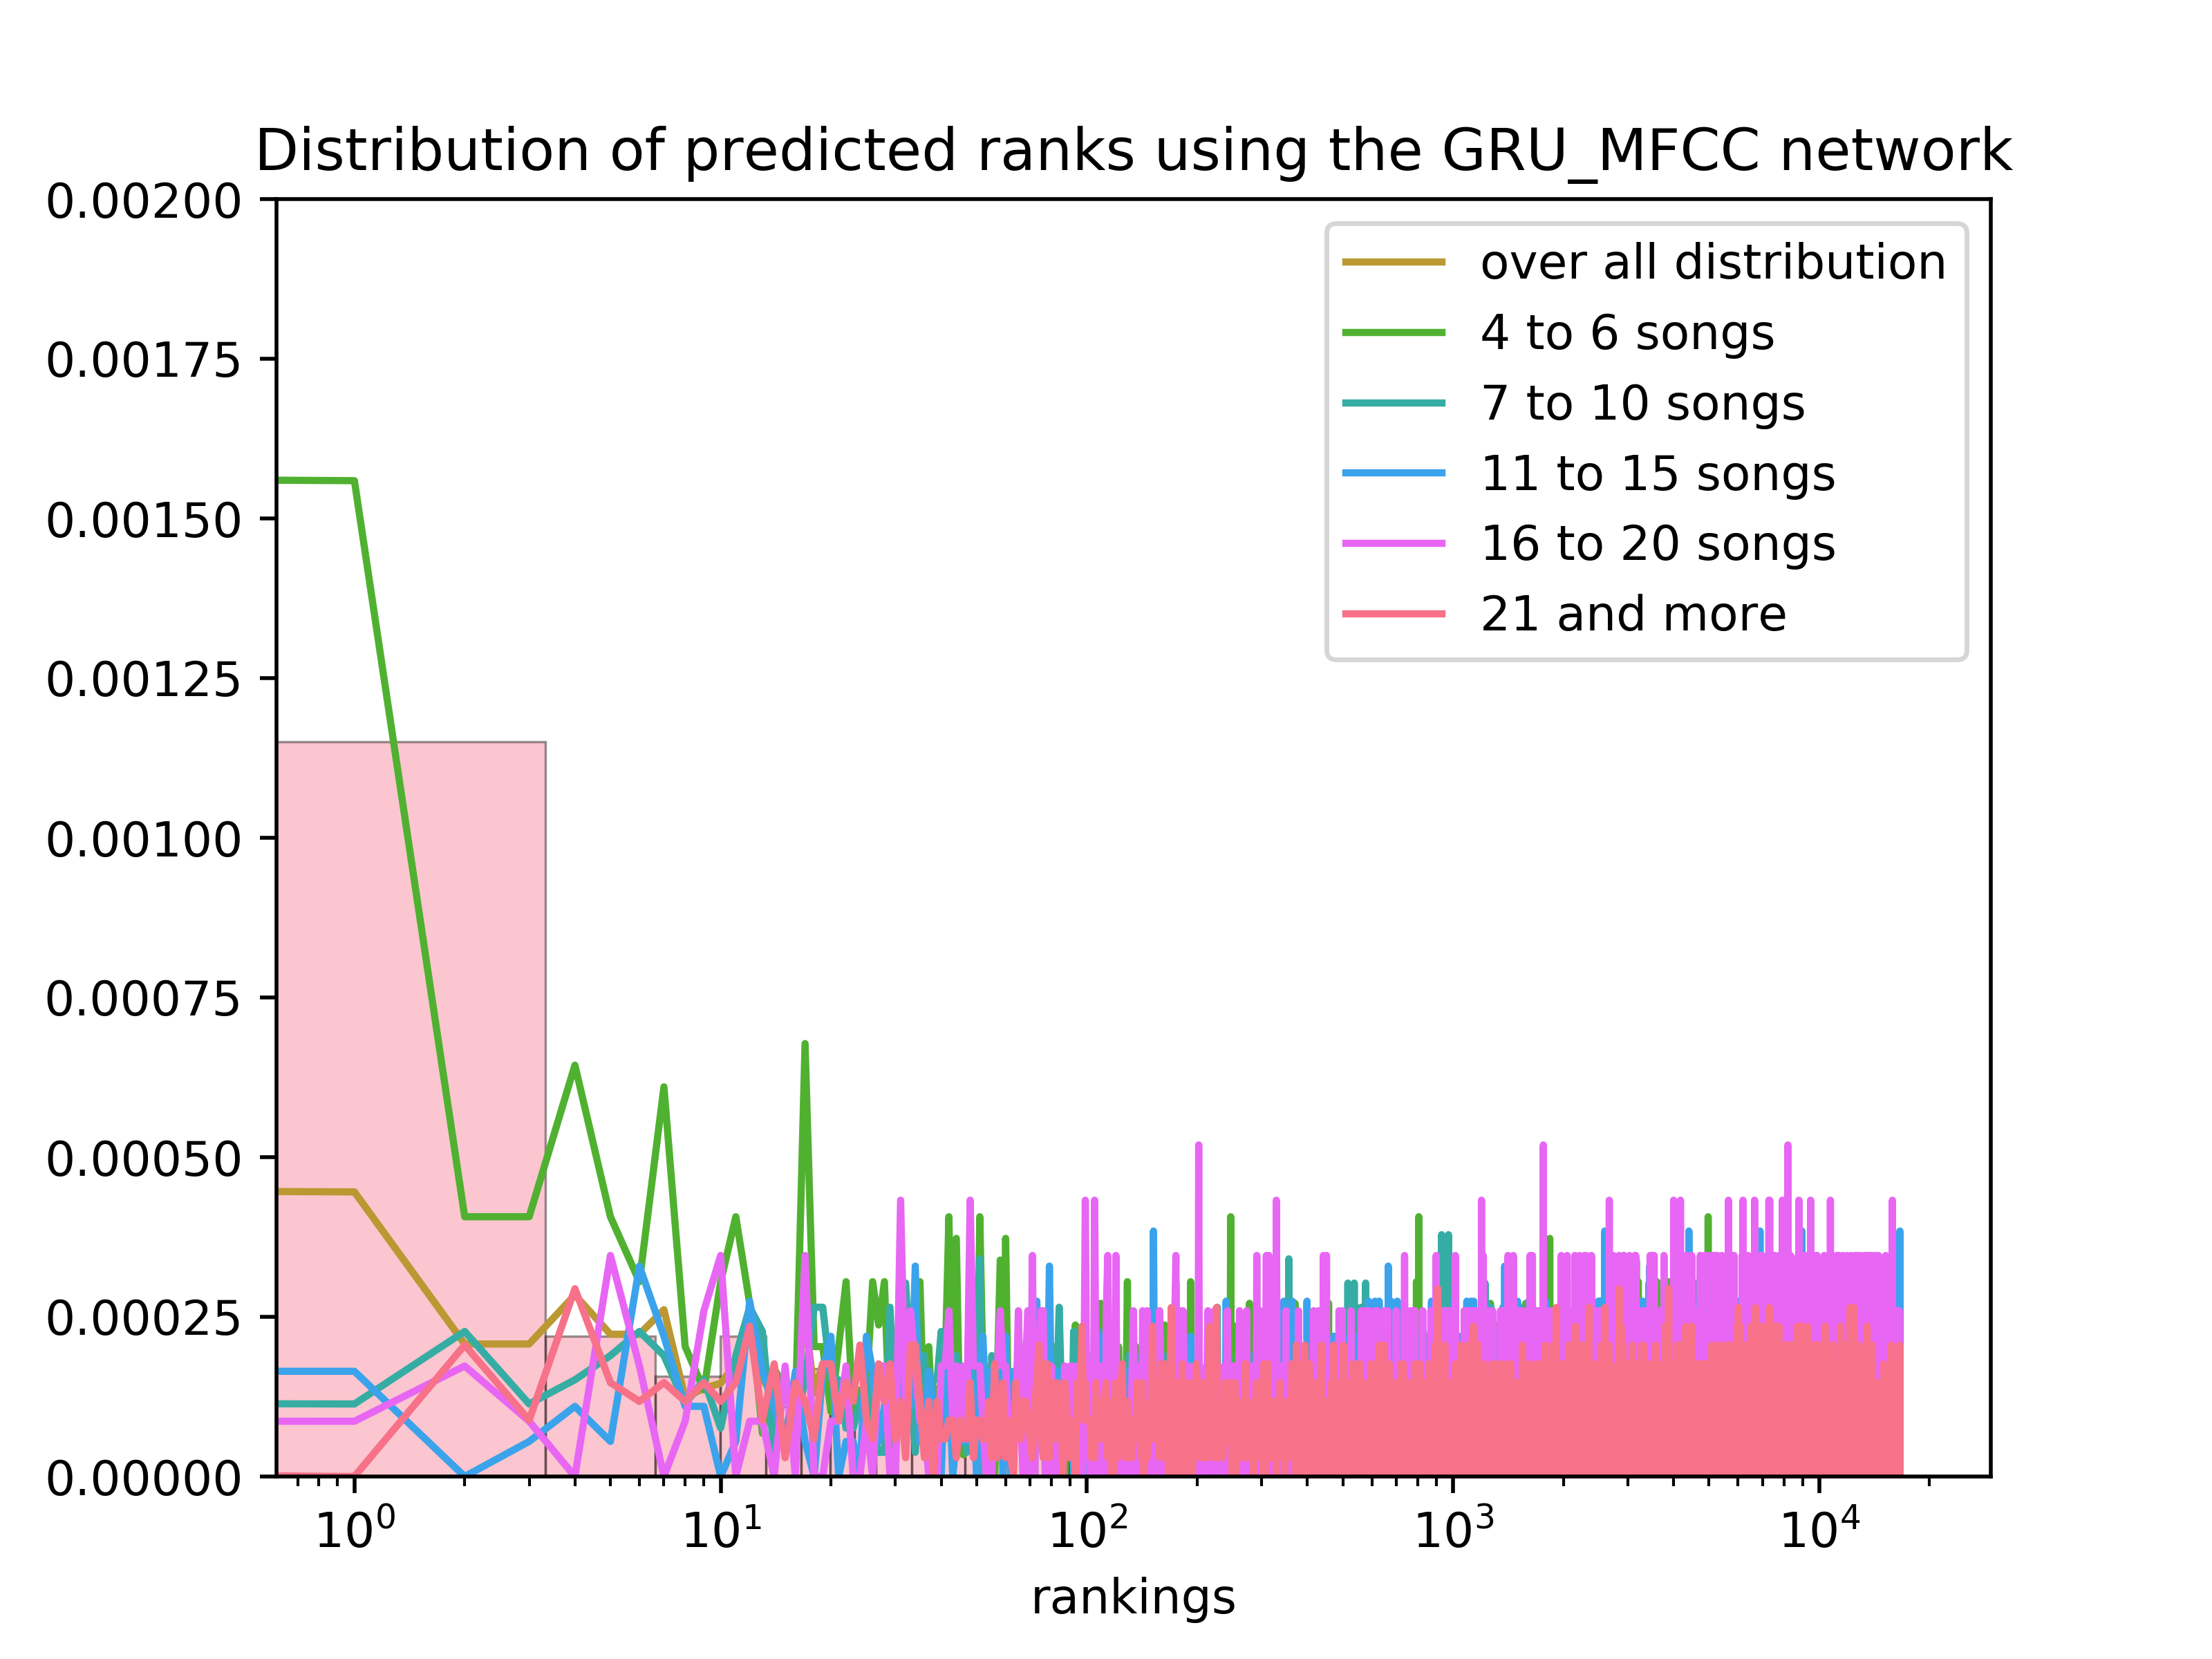
\includegraphics[width=1\linewidth]{./img/gru_mfcc_graph.png}
  \caption{The RDG of GRU\_MFCC}
  \label{fig:gru_mfcc_distribution}
\end{minipage}%
\begin{minipage}{.5\textwidth}
  \centering
  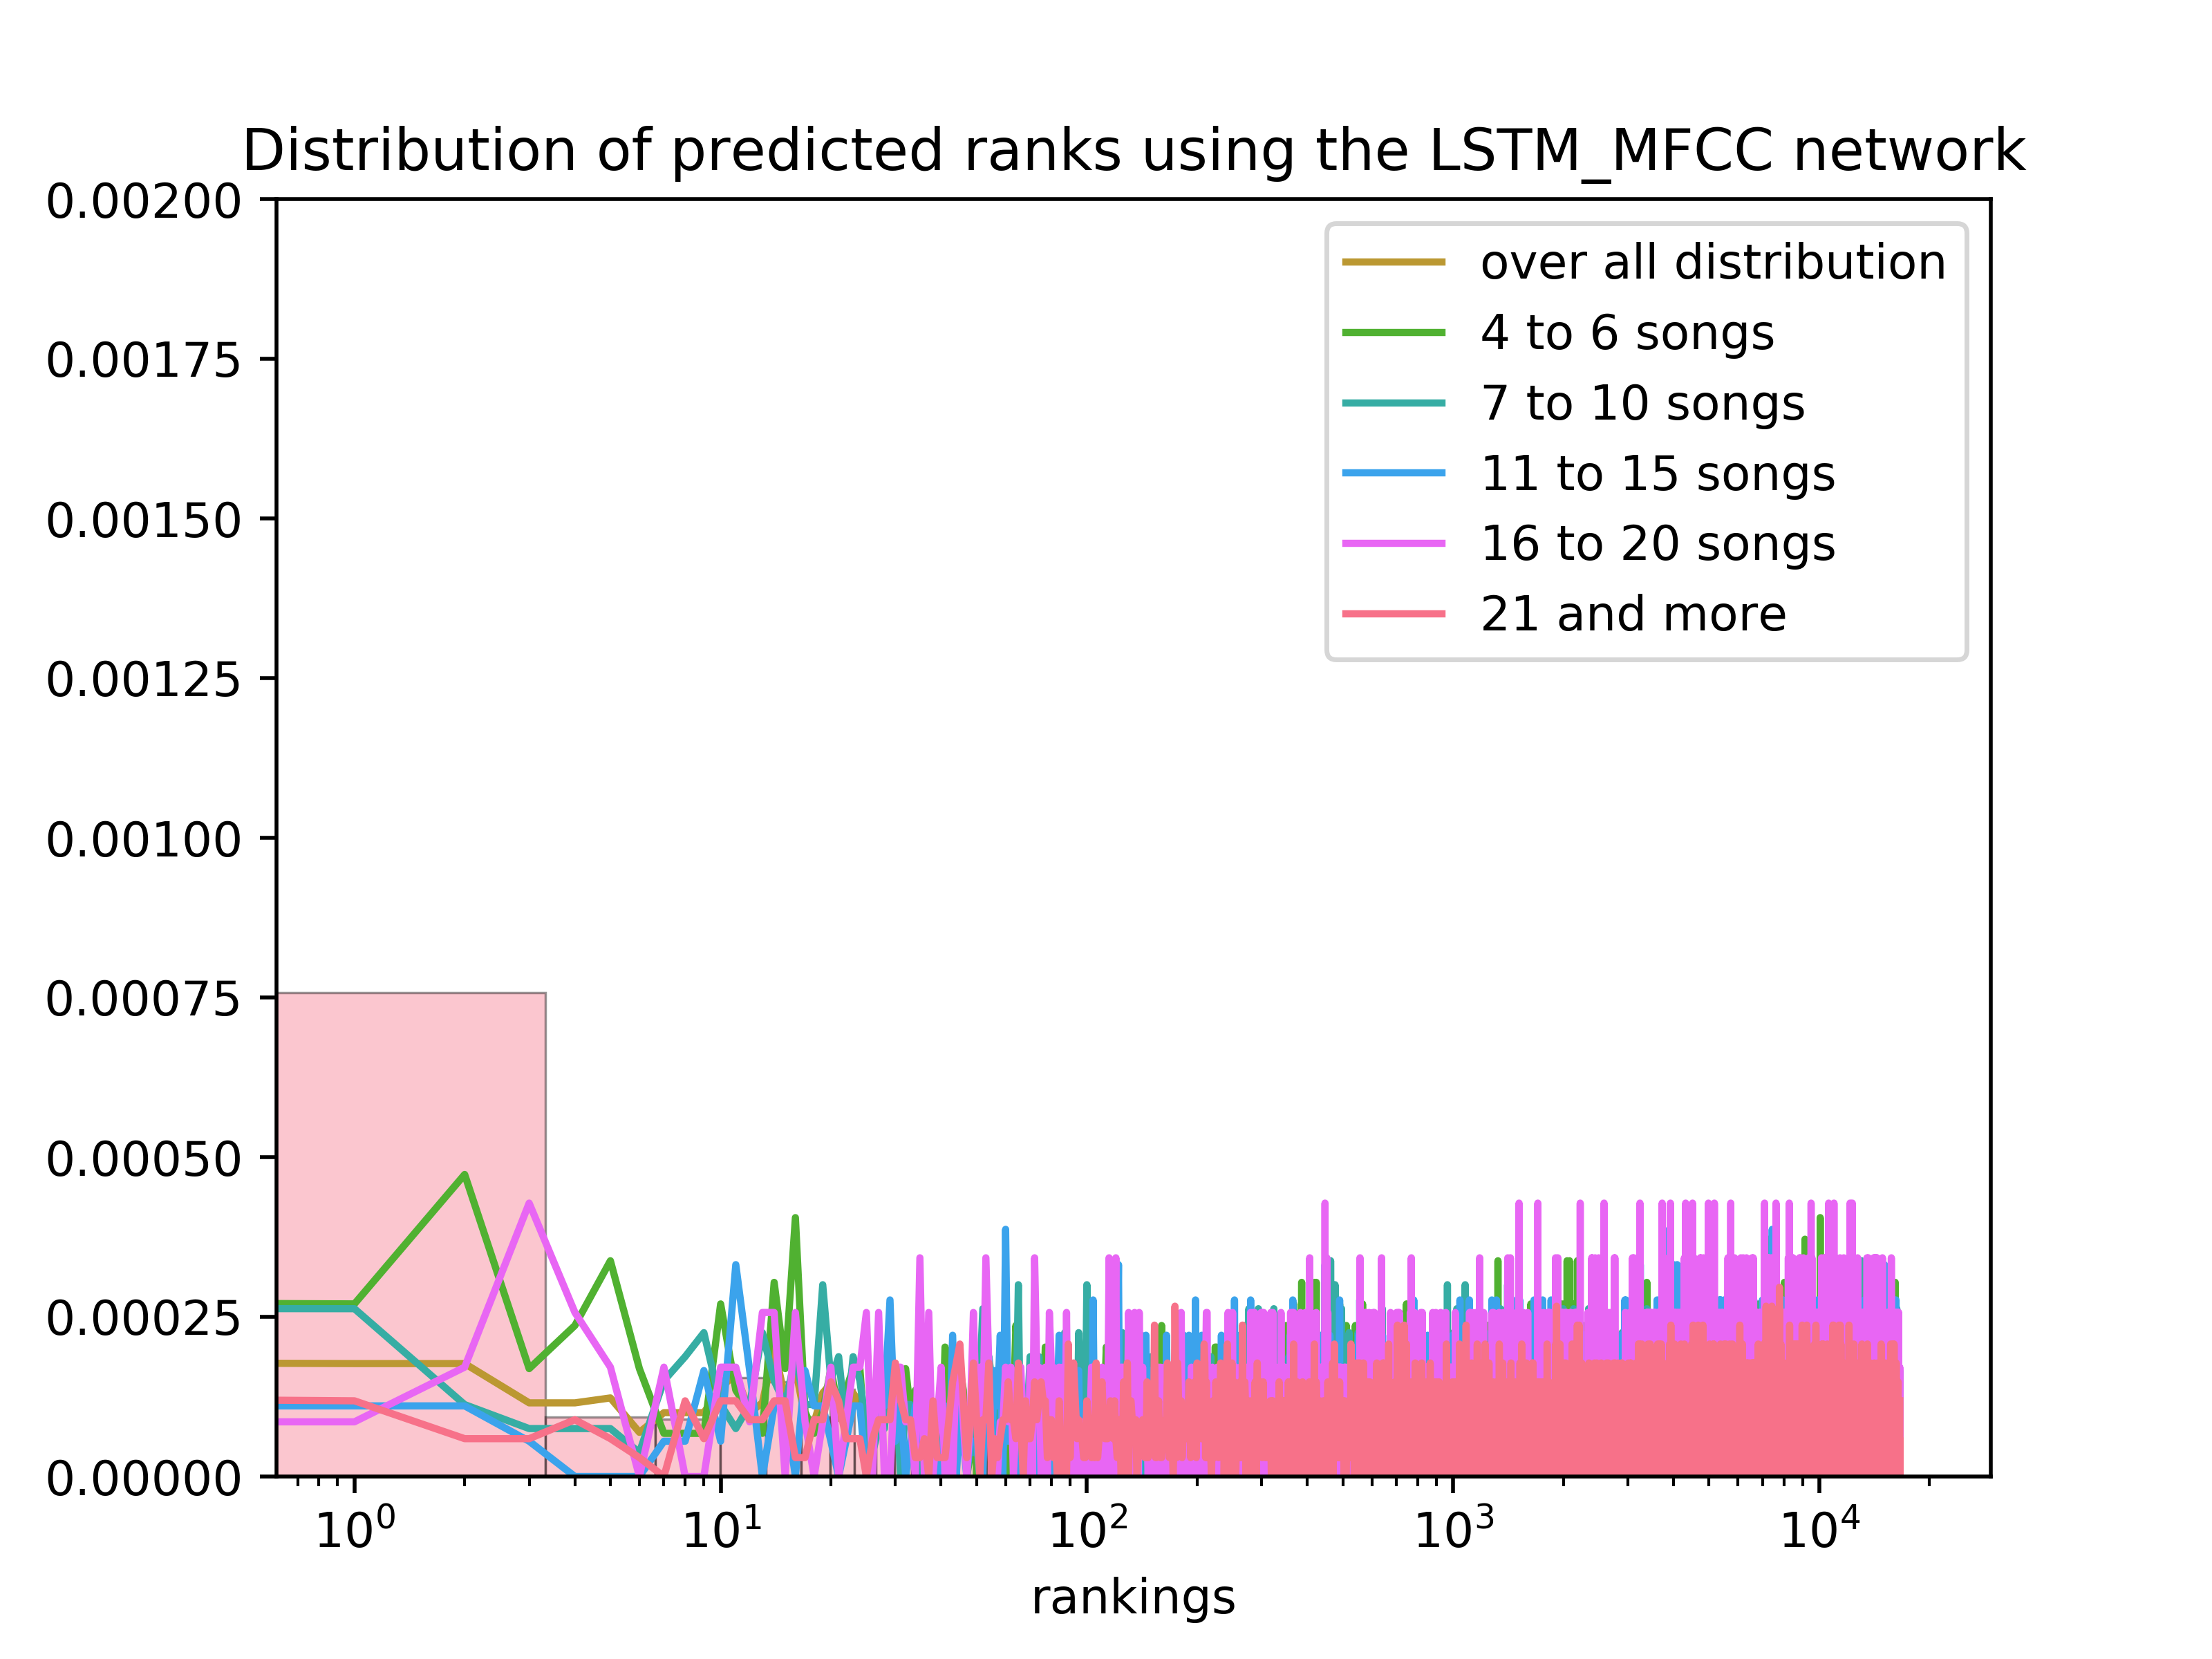
\includegraphics[width=1\linewidth]{./img/lstm_mfcc_graph.png}
  \caption{The RDG of LSMT\_MFCC}
  \label{fig:gru_mfcc_distribution}
\end{minipage}
\end{figure}\label{fig:mfcc_nn_distributions}



\section{Discussion}\label{sec:discussion}

All the experiments we performed yielded a lot of data, to be fair more than we planned. In this discussion we try to compare our findings with the expectations we had and interpret their similarities and differences. Overall we have to admit that the results we obtained were worse than we thought they were going to be. We will try to explain the reasons. \\
The thing that was apparent in almost all methods was the decrease of top ranking for songs from $ p_{test}$ that were a part of a longer playlist. We thought that this is actually a thing that we could fix. The fact that shorter playlists have better rankings suggests that the users have groups of songs in their playlists that are very similar to each other but the groups can be quite dissimilar and that songs, that are somewhat similar to all groups "pollute" the recommendations. Therefore, we decided to evaluate all methods again with a distance threshold. We actually meant to do this even before we knew that our methods perform better on shorter playlists because we thought that it is better not to save all distances into the web-applications database but only the top $n$. \\
We chose the threshold separately for each method as the 846297th biggest similarity. It may seem as a strange random number but is is $51*|dataset|$ where . It gives us about 50 most similar songs for each song and the additional 1 is to get 50 even though we will always include the most similar one which is the same one. \\
This significantly changed and in many cases improved the performances of our methods. We decided not to include all the new distribution graphs again, \todo{Mohla bych je dat do attachmentu} but we decided to include at least a table comparing the other evaluation measures we chose. \todo{SEM dat table nebo graf? tech novejch metod}.\\

Even with the threshold improvement, our results are still worse than we were hoping for. 
\begin{figure}[h]
    \centering
	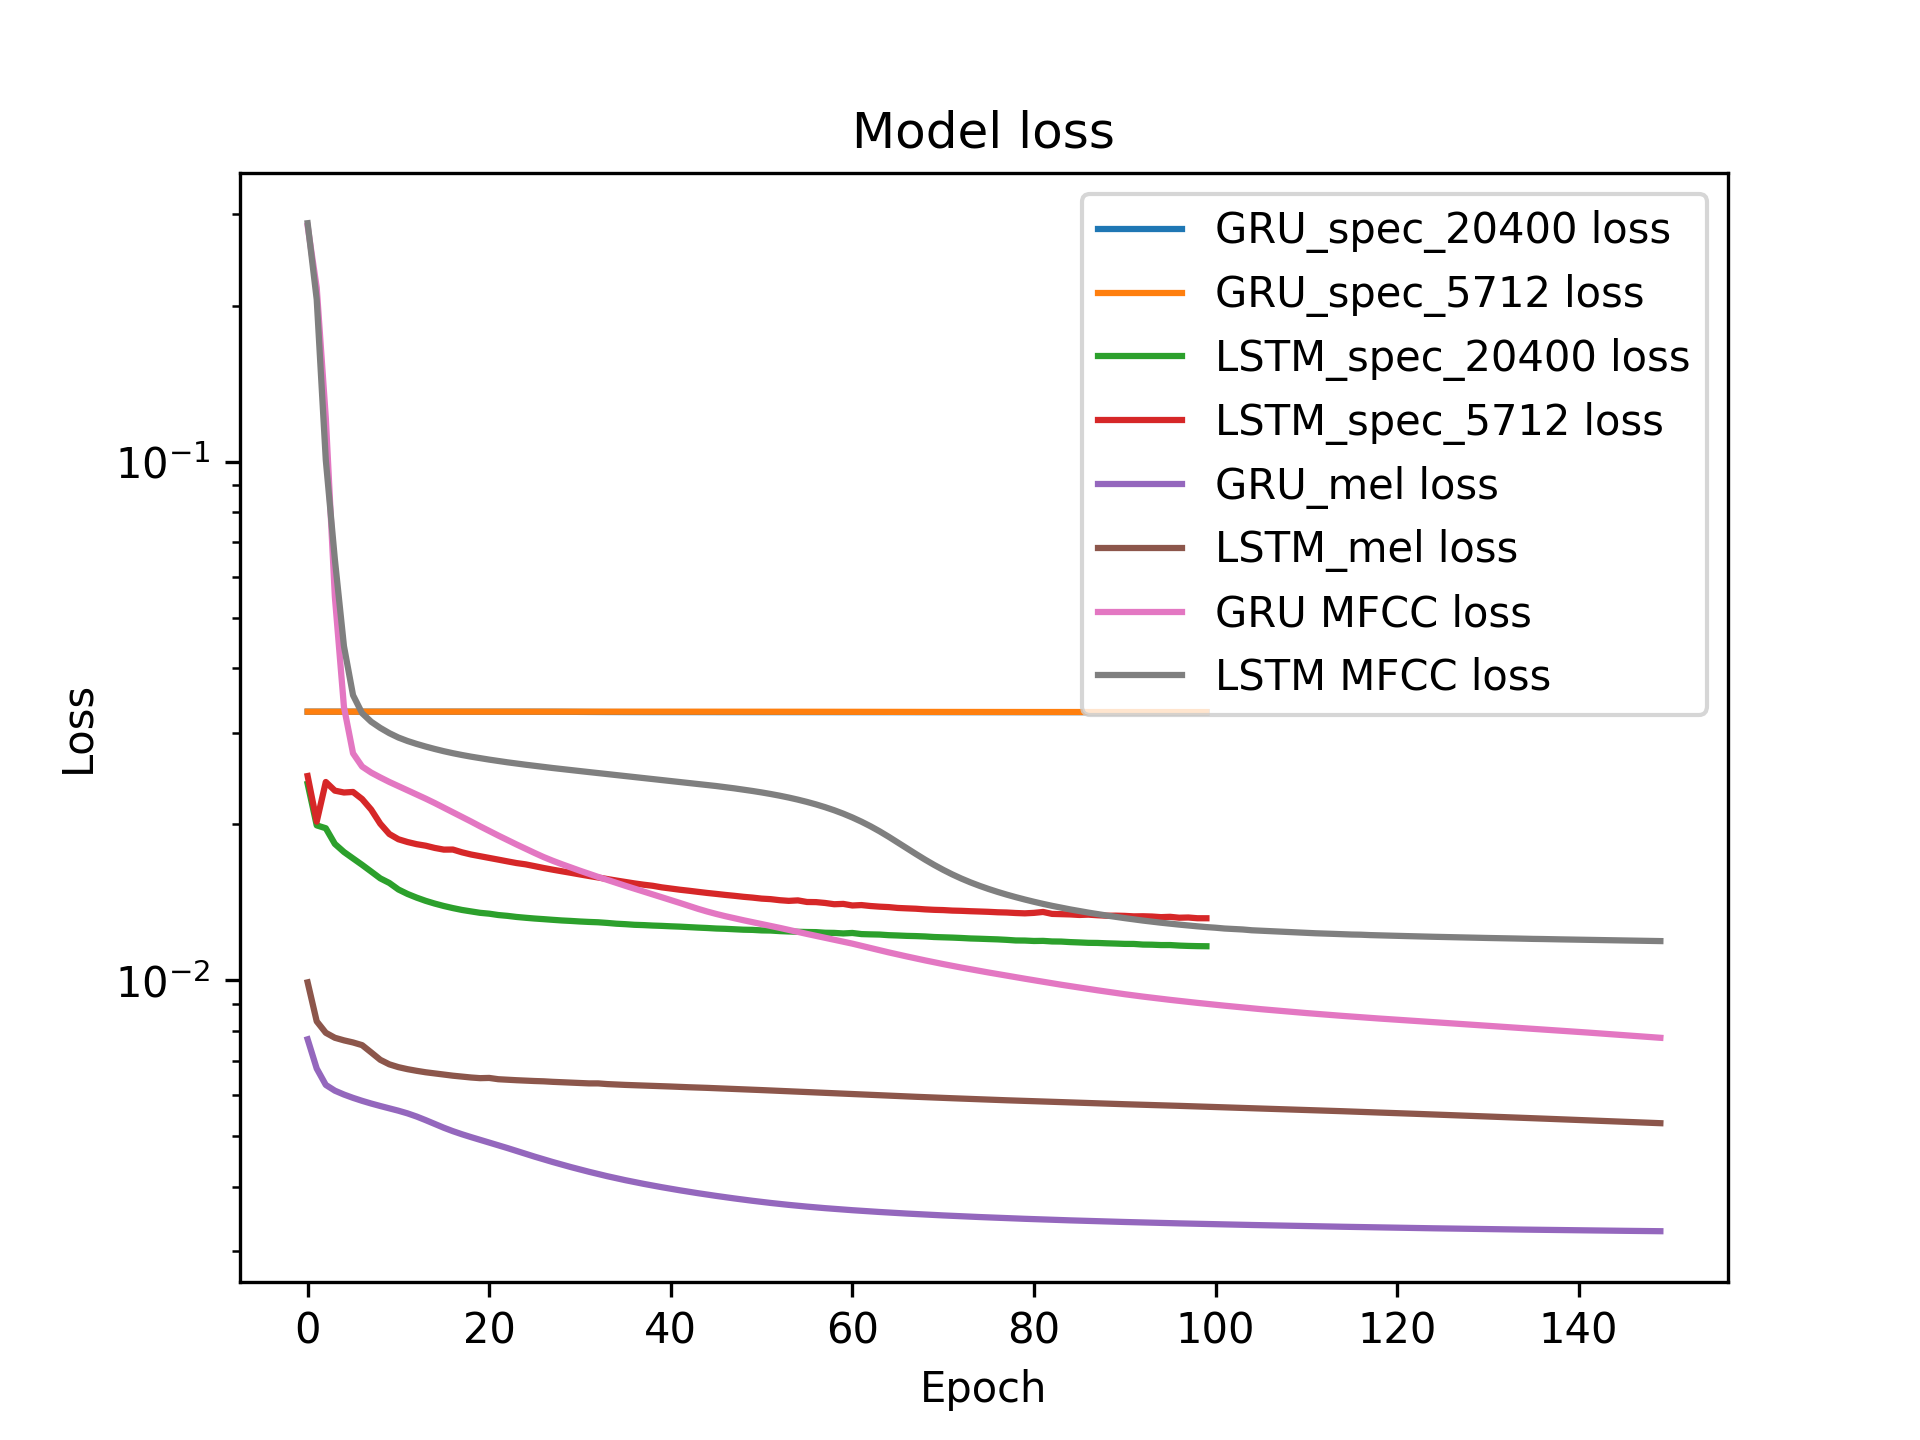
\includegraphics[width=120mm]{./img/all_training_graphs.png}
	\caption{The training mean squared error loss values for all the final neural networks we trained.}
	\label{fig:all_model_training}
\end{figure}